% !TeX program = lualatex
% Główny plik pracy inżynierskiej.
% Kompilacja: latexmk -lualatex main.tex

\documentclass[12pt,a4paper]{report}

% --- Język, fonty i kodowanie ---
\usepackage{fontspec}
\usepackage[english,polish]{babel}
\usepackage{csquotes}
\usepackage{indentfirst}

% --- Układ strony ---
\usepackage[a4paper,margin=2.5cm]{geometry}
\usepackage{setspace}
\onehalfspacing

% --- Matematyka, tabele, grafika ---
\usepackage{amsmath}
\usepackage{amssymb}
\usepackage{booktabs}
\usepackage{graphicx}
\usepackage{float}
\usepackage{subcaption}
\usepackage{tikz}
\usetikzlibrary{arrows.meta,positioning,shapes.geometric,shapes.misc,fit,calc}

% --- Linki i odwołania ---
\usepackage{xurl}
\usepackage[hidelinks]{hyperref}
\usepackage[nameinlink,noabbrev]{cleveref}
\crefname{chapter}{rozdział}{rozdziały}
\Crefname{chapter}{Rozdział}{Rozdziały}
\crefname{section}{sekcja}{sekcje}
\Crefname{section}{Sekcja}{Sekcje}
\crefname{figure}{rysunek}{rysunki}
\Crefname{figure}{Rysunek}{Rysunki}
\crefname{table}{tabela}{tabele}
\Crefname{table}{Tabela}{Tabele}
\crefname{equation}{równanie}{równania}
\Crefname{equation}{Równanie}{Równania}
\providecommand{\crefpairconjunction}{ i }
\providecommand{\crefmiddleconjunction}{, }
\providecommand{\creflastconjunction}{ i }

% --- Bibliografia ---
\usepackage[backend=biber,style=authoryear,sorting=nyt]{biblatex}
\addbibresource{references.bib}

% --- Ścieżki do grafik ---
\graphicspath{{figures/}}

% --- Dane strony tytułowej PJATK ---
\newcommand{\ThesisFaculty}{Wydział Informatyki}
\newcommand{\ThesisDepartment}{Katedra Baz Danych}
\newcommand{\ThesisSpecialization}{Specjalizacja Systemy inteligentne i Data Science}
\newcommand{\ThesisAuthor}{Jakub Melzacki}
\newcommand{\ThesisStudentId}{s27664}
\newcommand{\ThesisTitle}{Predykcja wyników profesjonalnych meczów League of Legends z wykorzystaniem systemów rankingowych i metamodelu uczenia maszynowego}
\newcommand{\ThesisType}{Praca inżynierska}
\newcommand{\ThesisSupervisor}{dr Dominik Deja}
\newcommand{\ThesisPlaceDate}{Warszawa, maj 2026}

\newcommand{\makepjatktitlepage}{%
\begin{titlepage}
    \thispagestyle{empty}
    \centering
    
\includegraphics[width=0.42\textwidth]{pjatk_logo.pdf}\par
    \vspace{1.6cm}

    {\large \ThesisFaculty\par}
    \vspace{1.0cm}
    {\large \ThesisDepartment\par}
    \vspace{0.6cm}
    {\large \ThesisSpecialization\par}

    \vfill

    {\large \ThesisAuthor\par}
    \vspace{0.2cm}
    {\large Nr albumu \ThesisStudentId\par}

    \vspace{1.8cm}

    {\Large\bfseries \ThesisTitle\par}

    \vfill

    {\large \ThesisType\par}
    \vspace{0.8cm}
    {\large \ThesisSupervisor\par}

    \vfill
    {\large \ThesisPlaceDate\par}
\end{titlepage}%
}

\begin{document}

\setcounter{secnumdepth}{3}
\setcounter{tocdepth}{3}

\makepjatktitlepage

\pagenumbering{roman}

\begin{abstract}
\hspace*{1.5em}Praca dotyczy predykcji wyników profesjonalnych meczów \textit{League of Legends} na podstawie historycznych danych sportowych oraz porównania jakości predykcji z benchmarkiem bukmacherskim. Wykorzystano dane GOL.GG oraz kursy z serwisu OddsPortal. Celem pracy było sprawdzenie, czy systemy rankingowe zawodników i drużyn mogą stanowić skuteczną bazę predykcyjną oraz czy metamodel rankingowo-kontekstowy poprawia jakość oceny wyniku meczu.

Porównano rodziny rankingów Elo, Glicko-2, TrueSkill, OpenSkill, Plackett--Luce oraz Thurstone--Mosteller. Ich predykcje, miary niepewności, pełny historyczny kontekst drużynowy W20 oraz sygnały skorygowane dwumianowo względem formatu serii wykorzystano w metamodelu W20-Binomial. Hiperparametry kilku rodzin estymatorów dobrano z użyciem Optuny, a finalne warianty oceniono chronologicznie w procedurze walk-forward, z użyciem metryk AUC, LogLoss, Brier score i ECE.

Wyniki wskazują, że modele zawodnicze są skuteczniejsze od modeli opartych wyłącznie na nazwach drużyn, a najlepszym pojedynczym rankingiem był Player Glicko-2. Najlepszym estymatorem finalnego zestawu cech okazała się regularyzowana regresja logistyczna ElasticNet. Wariant końcowy został dodatkowo usymetryzowany względem kolejności drużyn oraz skalibrowany metodą Platta w schemacie expanding-window. Skalibrowany symetryczny model LR-ElasticNet-W20-Binomial uzyskał niższy LogLoss niż pojedynczy ranking Player Glicko-2 oraz benchmarki Market Open i Market Close. Wynik należy interpretować jako przewagę predykcyjną na analizowanej próbie historycznej, a nie jako dowód opłacalności strategii zakładów.

\textbf{Słowa kluczowe:} League of Legends, esport, predykcja wyników, systemy rankingowe, Glicko-2, metamodel kontekstowy, W20-Binomial, regresja logistyczna ElasticNet, kursy bukmacherskie, LogLoss, kalibracja.
\end{abstract}

\begin{otherlanguage}{english}
\begin{abstract}
\hspace*{1.5em}This thesis addresses the problem of predicting outcomes of professional \textit{League of Legends} matches using historical sports data and compares the quality of these predictions with bookmaker benchmarks. The study uses GOL.GG data and betting odds collected from OddsPortal. The objective was to examine whether player- and team-based rating systems can provide an effective predictive foundation, and whether a ranking-context metamodel improves probabilistic match outcome estimation.

The analysis compares Elo, Glicko-2, TrueSkill, OpenSkill, Plackett--Luce and Thurstone--Mosteller rating families. Their predictions, uncertainty measures, full historical team context with a 20-match rolling window, and binomially adjusted signals dependent on series format were used in the W20-Binomial metamodel. Hyperparameters of several estimator families were selected with Optuna, while final variants were evaluated chronologically using a walk-forward procedure and the AUC, LogLoss, Brier score and ECE metrics.

The results indicate that player-based models outperform models based only on team names, and that Player Glicko-2 was the strongest single rating system. The best estimator for the final feature set was regularized ElasticNet logistic regression. The final variant was additionally symmetrized with respect to team ordering and calibrated with expanding-window Platt scaling. The calibrated symmetric LR-ElasticNet-W20-Binomial model achieved lower LogLoss than the single Player Glicko-2 ranking and the Market Open and Market Close bookmaker benchmarks. This result should be interpreted as a predictive advantage on the analysed historical sample, not as evidence of profitability of a betting strategy.

\textbf{Keywords:} League of Legends, esports, match outcome prediction, rating systems, Glicko-2, contextual metamodel, W20-Binomial, ElasticNet logistic regression, betting odds, LogLoss, calibration.
\end{abstract}
\end{otherlanguage}

\clearpage

\tableofcontents

\clearpage
\pagenumbering{arabic}

\chapter{Wstęp}

Dynamiczny rozwój esportu sprawił, że profesjonalne rozgrywki w grach komputerowych stały się
pełnoprawnym obszarem analizy ilościowej. Jednym z najgłośniejszych przykładów jest \textit{League
of Legends}, dla którego dostępne są wieloletnie dane o meczach, składach, statystykach gry oraz --
dla części spotkań -- kursach bukmacherskich. Taka kombinacja danych pozwala badać nie tylko to, czy
model potrafi wskazać zwycięzcę, lecz także czy potrafi przypisać realistyczne prawdopodobieństwo
wyniku.

Prognozowanie wyników takich meczów jest trudne, ponieważ obserwowana siła zespołu zmienia się w
czasie. Składy są przebudowywane, zawodnicy pełnią wyspecjalizowane role, a aktualizacje gry
wpływają na dominujące strategie. Dlatego sama historyczna nazwa drużyny jest często zbyt ubogą
reprezentacją jej bieżącego potencjału sportowego. W pracy przyjęto więc perspektywę przedmeczowej
predykcji probabilistycznej, w której model może korzystać wyłącznie z informacji dostępnych przed
rozpoczęciem spotkania.

Celem niniejszej pracy jest opracowanie oraz ocena modelu przewidującego wynik profesjonalnego meczu
\textit{League of Legends}. Model łączy systemy rankingowe zawodników, miary niepewności, pełny
historyczny kontekst drużynowy W20 oraz korektę dwumianową zależną od formatu serii Bo1/Bo3/Bo5.
Jako zewnętrzny punkt odniesienia wykorzystano prawdopodobieństwa implikowane przez kursy
bukmacherskie, które są jednym z najsilniejszych publicznie dostępnych benchmarków dla predykcji
przedmeczowej.

Praca nie dotyczy budowy systemu inwestycyjnego ani oceny opłacalności zakładów. Analiza ogranicza
się do jakości predykcji probabilistycznej, dlatego wykorzystano AUC, LogLoss, Brier Score oraz
Expected Calibration Error, przy czym główną metryką jest LogLoss.

Zakres pracy obejmuje analizę danych GOL.GG, przygotowanie wspólnej próby z kursami OddsPortal,
porównanie systemów rankingowych, budowę metamodelu W20-Binomial oraz końcową ocenę względem rynku
bukmacherskiego. Główna ewaluacja została przeprowadzona na meczach, dla których dostępne były oba
typy danych.

Główne pytanie badawcze pracy brzmi: czy model oparty na rankingach zawodników i historycznym
kontekście drużyn potrafi skutecznie przewidywać wyniki profesjonalnych meczów \textit{League of
Legends} oraz osiągać jakość probabilistyczną konkurencyjną względem kursów bukmacherskich?

W pracy przyjęto następujące hipotezy badawcze:

\begin{enumerate}
    \item Systemy rankingowe oparte na zawodnikach osiągają lepszą jakość predykcji niż systemy rankingowe oparte wyłącznie na drużynach.
    \item Metamodel łączący sygnały rankingowe poprawia jakość predykcji względem pojedynczego najlepszego systemu rankingowego.
    \item Dodanie historycznego kontekstu formy drużyn poprawia jakość probabilistyczną modelu względem wariantu opartego wyłącznie na rankingach.
    \item Model rankingowo-kontekstowy osiąga wyniki konkurencyjne względem prawdopodobieństw implikowanych przez kursy bukmacherskie.
\end{enumerate}

Dalsza część pracy została zorganizowana w następujący sposób. Najpierw przedstawiono stan wiedzy i
kontekst problemu, obejmujący predykcję sportową, systemy rankingowe, metamodelowanie, ocenę
probabilistyczną oraz rolę kursów bukmacherskich jako benchmarku. Następnie opisano środowisko
\textit{League of Legends}, wykorzystane źródła danych GOL.GG i OddsPortal oraz proces konstrukcji
wspólnej próby badawczej. Kolejny rozdział zawiera eksploracyjną analizę danych, obejmującą
strukturę zbioru, formaty meczów, poziomy rozgrywek oraz podstawową analizę rynku bukmacherskiego. W
dalszej części opisano metodykę ewaluacji, systemy rankingowe wykorzystane jako modele bazowe,
konstrukcję metamodelu W20-Binomial, dobór okna historycznego, porównanie rodzin estymatorów oraz
końcową symetryzację i kalibrację. Rozdział wynikowy prezentuje końcowe porównanie modeli, analizę
bootstrapową, segmentację według formatu serii i weryfikację hipotez. Następnie omówiono
interpretację wyników, ograniczenia badania oraz kierunki dalszych prac. Ostatni rozdział zawiera
syntetyczne podsumowanie i odpowiedź na pytanie badawcze.

\chapter{Stan wiedzy i kontekst problemu}

\section{Predykcja wyników w sporcie i esporcie}

\subsection{Od klasyfikacji zwycięzcy do predykcji probabilistycznej}

Predykcja wyniku meczu sportowego może być formułowana na kilka sposobów. Najprostszym wariantem jest klasyfikacja zwycięzcy, w której model zwraca jedną z klas. W niniejszej pracy problem jest jednak rozumiany szerzej: celem nie jest wyłącznie wskazanie bardziej prawdopodobnego zwycięzcy, lecz oszacowanie prawdopodobieństwa zwycięstwa jednej ze stron. Takie ujęcie jest istotne, ponieważ dwa modele o podobnej trafności klasyfikacyjnej mogą różnić się jakością przypisywanych prawdopodobieństw. Model może poprawnie porządkować mecze według faworyta, ale jednocześnie systematycznie zawyżać lub zaniżać pewność predykcji.

W zadaniach sportowych i esportowych probabilistyczna interpretacja wyniku ma szczególne znaczenie. Mecz jest zdarzeniem losowym zależnym od aktualnej dyspozycji zawodników, zmian składu, decyzji strategicznych, przewagi strony mapy, formatu serii oraz czynników niedostępnych w danych historycznych. Model, który przypisuje zbyt wysoką pewność pojedynczym predykcjom, może osiągać akceptowalną trafność, ale słabą jakość probabilistyczną. Dlatego w dalszej części pracy główną metryką jest LogLoss, a accuracy pełni co najwyżej rolę pomocniczą.

\subsection{Dominujący charakter prac dotyczących \textit{League of Legends}}

Literatura dotycząca predykcji w \textit{League of Legends} jest relatywnie młoda i w dużej części koncentruje się na informacjach dostępnych w trakcie gry albo na cechach blisko związanych z przebiegiem konkretnej mapy. Przykładowo prace dotyczące predykcji wyniku meczu, analizy cech zwycięstwa, doświadczenia graczy na bohaterach oraz predykcji w czasie rzeczywistym wykorzystują statystyki drużyn, wybory bohaterów, doświadczenie zawodników lub zmienne opisujące stan rozgrywki \parencite{lin2016lol,costa2021lol,do2021championExperience,junior2023lol}. Taki kierunek jest naturalny, ponieważ dane wewnątrz gry silnie opisują aktualną przewagę jednej ze stron.

Z perspektywy niniejszej pracy jest to jednak inny problem badawczy niż przedmeczowa predykcja probabilistyczna. Jeżeli model korzysta z informacji po rozpoczęciu mapy, takich jak złoto, zabójstwa, obiekty neutralne, kompozycje po drafcie albo bieżący stan mapy, to przewiduje wynik warunkowo względem już ujawnionej części meczu. W niniejszej pracy przyjęto ostrzejsze ograniczenie informacyjne: model powinien działać przed meczem, a więc bez znajomości przebiegu gry. Oznacza to, że większe znaczenie mają historyczna siła zawodników, skład drużyny, forma, region, liga, format serii oraz kontekst czasowy.

Ten podział wyznacza lukę badawczą. Istnieją prace analizujące \textit{League of Legends} i istnieją prace wykorzystujące systemy rankingowe w sporcie, ale znacznie rzadziej spotyka się połączenie: przedmeczowa predykcja profesjonalnych spotkań \textit{League of Legends}, ratingi liczone sekwencyjnie, metamodel probabilistyczny oraz porównanie z benchmarkiem rynku kursów. Niniejsza praca wpisuje się właśnie w tę lukę.

\subsection{Specyfika esportu i uzasadnienie ratingów zawodniczych}

Esport różni się od tradycyjnych dyscyplin sportowych kilkoma cechami istotnymi dla modelowania. Po pierwsze, środowisko gry zmienia się wraz z aktualizacjami, które mogą wpływać na wartość strategii, bohaterów i stylów gry. Po drugie, drużyny często modyfikują składy pomiędzy sezonami, a pojedynczy zawodnik może mieć duży wpływ na siłę zespołu. Po trzecie, profesjonalne rozgrywki są podzielone na ligi, turnieje i regiony o różnym poziomie sportowym. Te czynniki powodują, że model oparty wyłącznie na nazwie drużyny może być niestabilny, szczególnie przy transferach zawodników.

Z tego powodu uzasadnione jest wykorzystanie rankingów zawodniczych jako podstawowego sygnału. Ranking zawodnika może przenosić część informacji pomiędzy drużynami po transferze i pozwala oddzielić bieżącą siłę składu od historycznej marki organizacji. Jednocześnie ranking sam w sobie nie opisuje pełnego kontekstu meczu: nie zawiera bezpośrednio informacji o formie w ostatnich spotkaniach, stylu gry, ekonomii, czasie trwania map ani formacie serii. Te ograniczenia motywują budowę metamodelu łączącego rankingi z historycznymi agregatami drużynowymi.

\section{Systemy rankingowe jako modele siły uczestników}

\subsection{Elo jako punkt wyjścia dla modeli ratingowych}

Jednym z najbardziej znanych sposobów modelowania siły uczestników rywalizacji jest system Elo, pierwotnie zaproponowany dla szachów \parencite{elo1978}. Podstawowa idea polega na przypisaniu każdemu graczowi liczbowej oceny siły, która jest aktualizowana po kolejnych wynikach. Różnica ratingów jest przekształcana na oczekiwane prawdopodobieństwo zwycięstwa, a następnie ratingi są korygowane zależnie od tego, czy wynik był zgodny z oczekiwaniem.

Popularność Elo wynika z prostoty, interpretowalności i możliwości działania online. Model nie wymaga pełnego ponownego trenowania po każdym meczu, lecz aktualizuje oceny sekwencyjnie. Ta cecha jest szczególnie użyteczna w danych sportowych i esportowych, gdzie obserwacje pojawiają się chronologicznie, a siła uczestników może zmieniać się w czasie.

\subsection{Elo w predykcji piłki nożnej}

Zastosowanie Elo do piłki nożnej badali między innymi Hvattum i Arntzen \parencite{hvattum2010eloFootball}. Autorzy wykorzystali ratingi Elo jako źródło zmiennych w uporządkowanych modelach logitowych predykcji wyniku meczu. Istotne jest tutaj nie samo użycie rankingu jako tabeli siły zespołów, lecz przekształcenie różnicy ratingów w predykcję probabilistyczną i porównanie takiego podejścia z innymi metodami.

Wyniki tej pracy są ważnym argumentem metodologicznym dla niniejszego projektu. Pokazują, że rating historyczny może być używany jako sygnał predykcyjny w modelu statystycznym, a nie tylko jako opisowa miara pozycji drużyny. Jednocześnie późniejsze omówienia tego nurtu wskazują, że modele oparte wyłącznie na Elo mogą być słabsze od kursów bukmacherskich, które agregują więcej informacji rynkowej \parencite{wunderlich2018bettingOddsRating}. Wniosek dla niniejszej pracy jest następujący: ratingi są silnym, interpretowalnym punktem wyjścia, ale nie powinny być traktowane jako pełny opis meczu. Dlatego w dalszych rozdziałach ratingi są porównywane jako samodzielne benchmarki, a następnie używane jako cechy metamodelu.

\subsection{Rozszerzenia probabilistyczne: Glicko-2, TrueSkill i OpenSkill}

Klasyczny Elo reprezentuje siłę jedną liczbą, ale nie opisuje jawnie niepewności tej oceny. W praktyce dwie drużyny lub dwóch zawodników z takim samym ratingiem mogą różnić się wiarygodnością oszacowania: jedna ocena może wynikać z wielu aktualnych meczów, a druga z małej liczby starych obserwacji. System Glicko oraz jego rozwinięcie Glicko-2 dodają do ratingu miarę niepewności, dzięki czemu aktualizacja może zależeć od pewności ocen uczestników \parencite{glickman1995,glickman2012}.

Inną rodziną metod są bayesowskie systemy ratingowe, takie jak TrueSkill \parencite{trueskill2007}, algorytmy online opisane przez Wenga i Lina \parencite{weng2011onlineRanking} oraz OpenSkill \parencite{openskill2024}. Ich wspólną cechą jest traktowanie siły uczestnika jako zmiennej losowej, a nie pojedynczej deterministycznej wartości. Taka reprezentacja jest atrakcyjna w esporcie, ponieważ pozwala modelowi odróżnić drużyny stabilne od drużyn, których poziom jest słabo rozpoznany.

W niniejszej pracy ratingi nie są traktowane wyłącznie jako końcowe modele. Pełnią dwie role. Po pierwsze, są oceniane jako samodzielne benchmarki predykcyjne. Po drugie, ich predykcje i parametry, w tym miary niepewności, stają się wejściem metamodelu. Takie podejście zachowuje interpretowalność rankingów, a jednocześnie pozwala modelowi wyższego poziomu łączyć wiele powiązanych sygnałów.

\section{Prace łączące ratingi z kursami bukmacherskimi}

\subsection{Ratingi i regresja logistyczna}

Prace sportowe oparte na ratingach są ważnym punktem odniesienia, ponieważ analizują podobną strukturę problemu: siła uczestników zmienia się w czasie, predykcja musi być wykonywana przed meczem, a wynik jest oceniany probabilistycznie. Thegelström \parencite{thegelstrom2023eloPremierLeagueOdds} analizował zastosowanie systemu Elo oraz regresji logistycznej do prognozowania kursów Premier League. Z perspektywy niniejszej pracy istotne są trzy elementy tego podejścia: rating jest aktualizowany chronologicznie, różnica ratingów staje się wejściem modelu statystycznego, a wyniki są interpretowane w odniesieniu do rynku kursów.

Podobieństwo do niniejszej pracy dotyczy więc ogólnej architektury: rating sekwencyjny + model probabilistyczny + benchmark rynkowy. Różnice są jednak równie ważne. W niniejszym projekcie ratingi są liczone nie tylko na poziomie drużyn, lecz także na poziomie zawodników, co jest uzasadnione transferami i rolami w \textit{League of Legends}. Ponadto końcowy model nie wykorzystuje pojedynczego ratingu, lecz łączy wiele rodzin rankingów, miary niepewności oraz kontekst historyczny W20.

\subsection{Betting Odds Rating System}

Najbardziej bezpośrednim przykładem połączenia ratingów i kursów jest praca Wunderlicha i Memmerta \parencite{wunderlich2018bettingOddsRating}. Autorzy zaproponowali Betting Odds Rating System, w którym informacje zawarte w kursach są wykorzystywane do aktualizacji oceny siły drużyn. Badanie objęło 14931 meczów z sezonów 2007/2008--2016/2017 w kilku rozgrywkach piłkarskich: Premier League, Bundeslidze, La Liga, Serie A oraz europejskich pucharach. Kursy zostały znormalizowane w celu usunięcia marży bukmacherskiej, a następnie porównano kilka wariantów: klasyczny model oparty na wyniku, wariant uwzględniający bramki oraz wariant oparty na kursach.

Wyniki pokazały, że kursy bukmacherskie były najsilniejszym punktem odniesienia pod względem średniej straty informacyjnej: dla samych kursów raportowano wartość 1.380, dla ELO-Odds 1.391, dla ELO-Goals 1.401, a dla ELO-Result 1.403. Oznacza to, że wariant wykorzystujący informację z kursów był lepszy od wariantów aktualizowanych wyłącznie wynikiem lub bramkami, ale nadal nie przewyższył bezpośrednio samych kursów jako prognozy. Dla niniejszej pracy jest to ważne ostrzeżenie: rynek kursów jest bardzo silnym benchmarkiem probabilistycznym, więc przewaga nad nim wymaga starannej ewaluacji na wspólnej próbie i z kontrolą niepewności.

Autorzy podkreślają również różnicę pomiędzy jakością predykcyjną a strategią finansową. Model może być użyteczny jako probabilistyczny opis siły drużyn, nawet jeśli nie tworzy bezpośrednio opłacalnej strategii zakładów. Ten wniosek jest zgodny z zakresem niniejszej pracy: kursy są traktowane jako benchmark prawdopodobieństw, a nie jako punkt wyjścia do analizy zysku, stawek lub zarządzania kapitałem.

\section{Metamodelowanie i łączenie sygnałów}

\subsection{Stacking jako rama metodologiczna}

Pojedynczy ranking może dobrze opisywać relatywną siłę zawodników, ale zwykle pomija część kontekstu. Z drugiej strony cechy historyczne drużyny mogą zawierać informacje o stylu gry i formie, lecz są podatne na szum oraz zmiany składu. Naturalnym rozwiązaniem jest połączenie wielu źródeł informacji w modelu drugiego poziomu.

Podejście to jest zgodne z ideą stacked generalization \parencite{wolpert1992} oraz stacked regressions \parencite{breiman1996stacked}. W takim schemacie predykcje modeli bazowych mogą być traktowane jako cechy wejściowe dla metamodelu. W niniejszej pracy model drugiego poziomu nie zastępuje rankingów, lecz uczy się, jak łączyć ich predykcje, niepewności oraz kontekst historyczny W20.

Wybór regresji logistycznej ElasticNet jako finalnego estymatora jest zgodny z charakterem problemu. Cechy rankingowe są silnie skorelowane, ponieważ wiele systemów opisuje tę samą ukrytą siłę sportową. Regularyzacja pozwala ograniczyć niestabilność współczynników i zmniejszyć ryzyko przeuczenia, a jednocześnie zachowuje większą interpretowalność niż modele drzewiaste lub głębokie sieci neuronowe.

\section{Ocena probabilistyczna i kalibracja}

\subsection{Właściwe reguły punktacji}

Ponieważ celem pracy jest oszacowanie prawdopodobieństwa zwycięstwa, metryka oceny powinna nagradzać poprawne prawdopodobieństwa, a nie tylko poprawną klasę. LogLoss oraz Brier Score należą do rodziny reguł punktacji używanych do oceny prognoz probabilistycznych. Właściwe reguły punktacji zachęcają model do raportowania prawdziwych przekonań probabilistycznych, ponieważ zaniżanie lub zawyżanie pewności jest karane \parencite{gneiting2007}.

LogLoss jest szczególnie istotny, ponieważ silnie karze sytuacje, w których model przypisuje wysokie prawdopodobieństwo błędnemu wynikowi. Jest to pożądane w analizie przedmeczowej, gdzie nadmierna pewność może być bardziej szkodliwa niż umiarkowana niepewność. Brier Score pełni funkcję pomocniczą, ponieważ mierzy średni kwadratowy błąd prawdopodobieństwa. AUC ocenia zdolność rozróżniania meczów, ale nie wystarcza do oceny jakości samych prawdopodobieństw.

\subsection{Kalibracja prawdopodobieństw}

Model może dobrze porządkować obserwacje, ale nadal generować źle skalibrowane prawdopodobieństwa. Kalibracja oznacza zgodność pomiędzy deklarowanym prawdopodobieństwem a empiryczną częstością zdarzenia. Jeżeli model w grupie predykcji około 70\% wygrywa w rzeczywistości tylko w 60\% przypadków, to jest nadmiernie pewny.

Do klasycznych metod poprawy kalibracji należą skalowanie Platta i kalibracja izotoniczna \parencite{zadrozny2002calibration,niculescu2005probabilities}. W nowszej literaturze zwraca się również uwagę, że modele o wysokiej trafności mogą być słabo skalibrowane, dlatego kalibracja powinna być analizowana osobno \parencite{guo2017calibration}. W niniejszej pracy kalibracja jest wykonywana w schemacie expanding-window, aby uniknąć przecieku informacji z przyszłości.

\section{Wnioski dla niniejszej pracy}

Przegląd literatury prowadzi do kilku decyzji projektowych. Po pierwsze, w pracach dotyczących \textit{League of Legends} dominują zadania wykorzystujące informacje dostępne w trakcie gry lub po jej rozpoczęciu, dlatego przedmeczowa predykcja probabilistyczna wymaga osobnego ujęcia. Po drugie, systemy rankingowe są naturalnym punktem wyjścia, ponieważ umożliwiają sekwencyjne śledzenie zmiennej siły zawodników i drużyn. Po trzecie, ratingi powinny być analizowane probabilistycznie, a nie wyłącznie jako ranking porządkowy. Po czwarte, kursy bukmacherskie są silnym benchmarkiem, ale ich użycie w tej pracy dotyczy jakości prawdopodobieństw, a nie strategii finansowej. Po piąte, metamodelowanie pozwala połączyć wiele rodzin rankingów z kontekstem historycznym, co odpowiada złożoności profesjonalnego esportu.

Te założenia wyznaczają dalszą strukturę pracy. Kolejne rozdziały opisują dane GOL.GG i OddsPortal, eksploracyjną analizę danych, metodykę ewaluacji, systemy rankingowe, konstrukcję metamodelu oraz końcowe porównanie z benchmarkami rynkowymi.

\input{chapters/01_dane_i_opis_zjawiska}
\chapter{Eksploracyjna analiza danych}

\section{Cel analizy eksploracyjnej}

Eksploracyjna analiza danych służy rozpoznaniu struktury próby przed budową modeli. W pracy ma trzy funkcje: sprawdza zróżnicowanie danych w czasie, formacie serii i poziomie rozgrywek, kontroluje balans zmiennej objaśnianej oraz wstępnie ocenia siłę rynku bukmacherskiego jako benchmarku.

EDA nie zastępuje eksperymentów modelowych. Uzasadnia natomiast późniejsze decyzje: walidację chronologiczną, segmentację Bo1/Bo3/Bo5, kontrolę poziomu rozgrywek oraz rozdzielenie kursów otwarcia i zamknięcia.

\section{Zakres czasowy i charakter próbki}

Dane sportowe obejmują wiele sezonów profesjonalnych rozgrywek \textit{League of Legends}. Jest to korzystne dla systemów rankingowych, ale oznacza także niejednorodność: w czasie zmieniały się składy, formaty rozgrywek, liczba turniejów oraz sama gra.

Z tego powodu w dalszej części pracy nie stosuje się losowego podziału obserwacji na zbiór treningowy i testowy. Taki podział mógłby prowadzić do sytuacji, w której model uczy się na meczach rozegranych po spotkaniach znajdujących się w zbiorze testowym. Zamiast tego zastosowano podejście chronologiczne, w którym predykcja dla danego meczu może korzystać jedynie z informacji dostępnych przed jego rozegraniem.

Wspólna próbka sportowo-rynkowa jest mniejsza od pełnej historii GOL.GG, ale tylko ona pozwala bezpośrednio porównać model z rynkiem. Dlatego w EDA dodatkowo sprawdzono, czy mecze z kursami nie są nadmiernie skupione na jednym poziomie rozgrywek.

\begin{figure}[H]
    \centering
    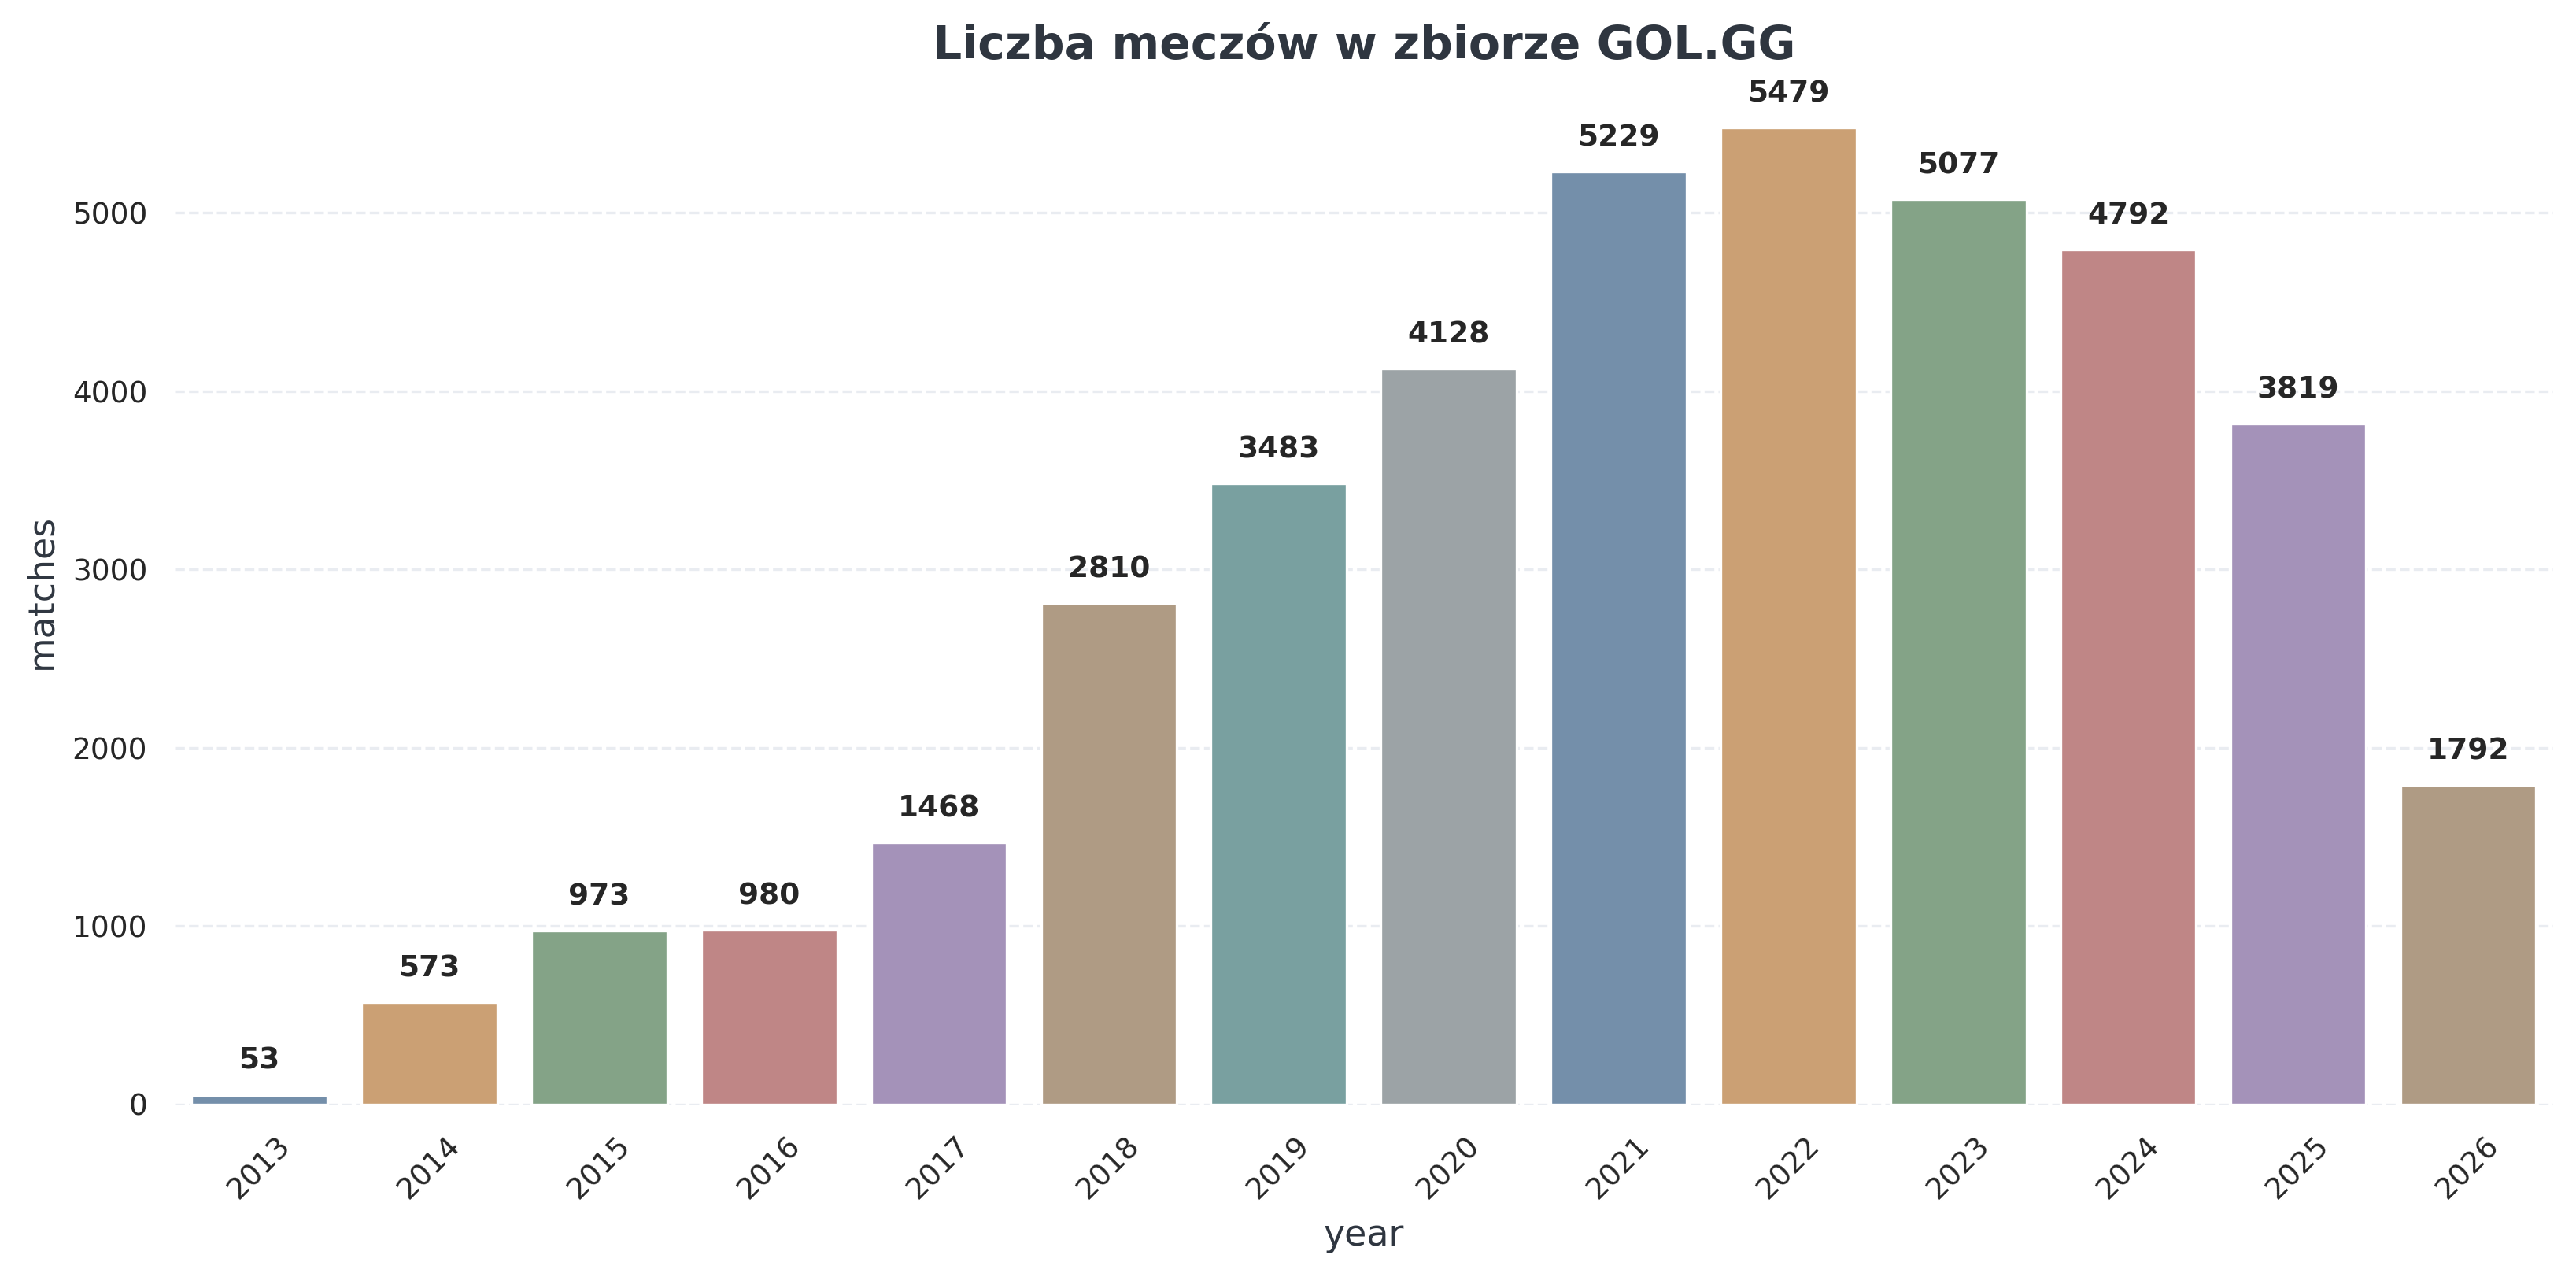
\includegraphics[width=0.9\textwidth]{eda_point4/sport_matches_per_year.png}
    \caption{Liczba meczów sportowych w kolejnych latach w danych GOL.GG.}
    \label{fig:eda_matches_per_year}
\end{figure}

\Cref{fig:eda_matches_per_year} pokazuje, że liczba obserwacji meczowych zmienia się w czasie. Sam wykres meczów nie opisuje jednak w pełni aktywności sceny esportowej, ponieważ pojedynczy mecz może składać się z jednej, trzech lub pięciu gier. Z tego powodu obok liczby meczów należy analizować także liczbę pojedynczych gier.

\begin{figure}[H]
    \centering
    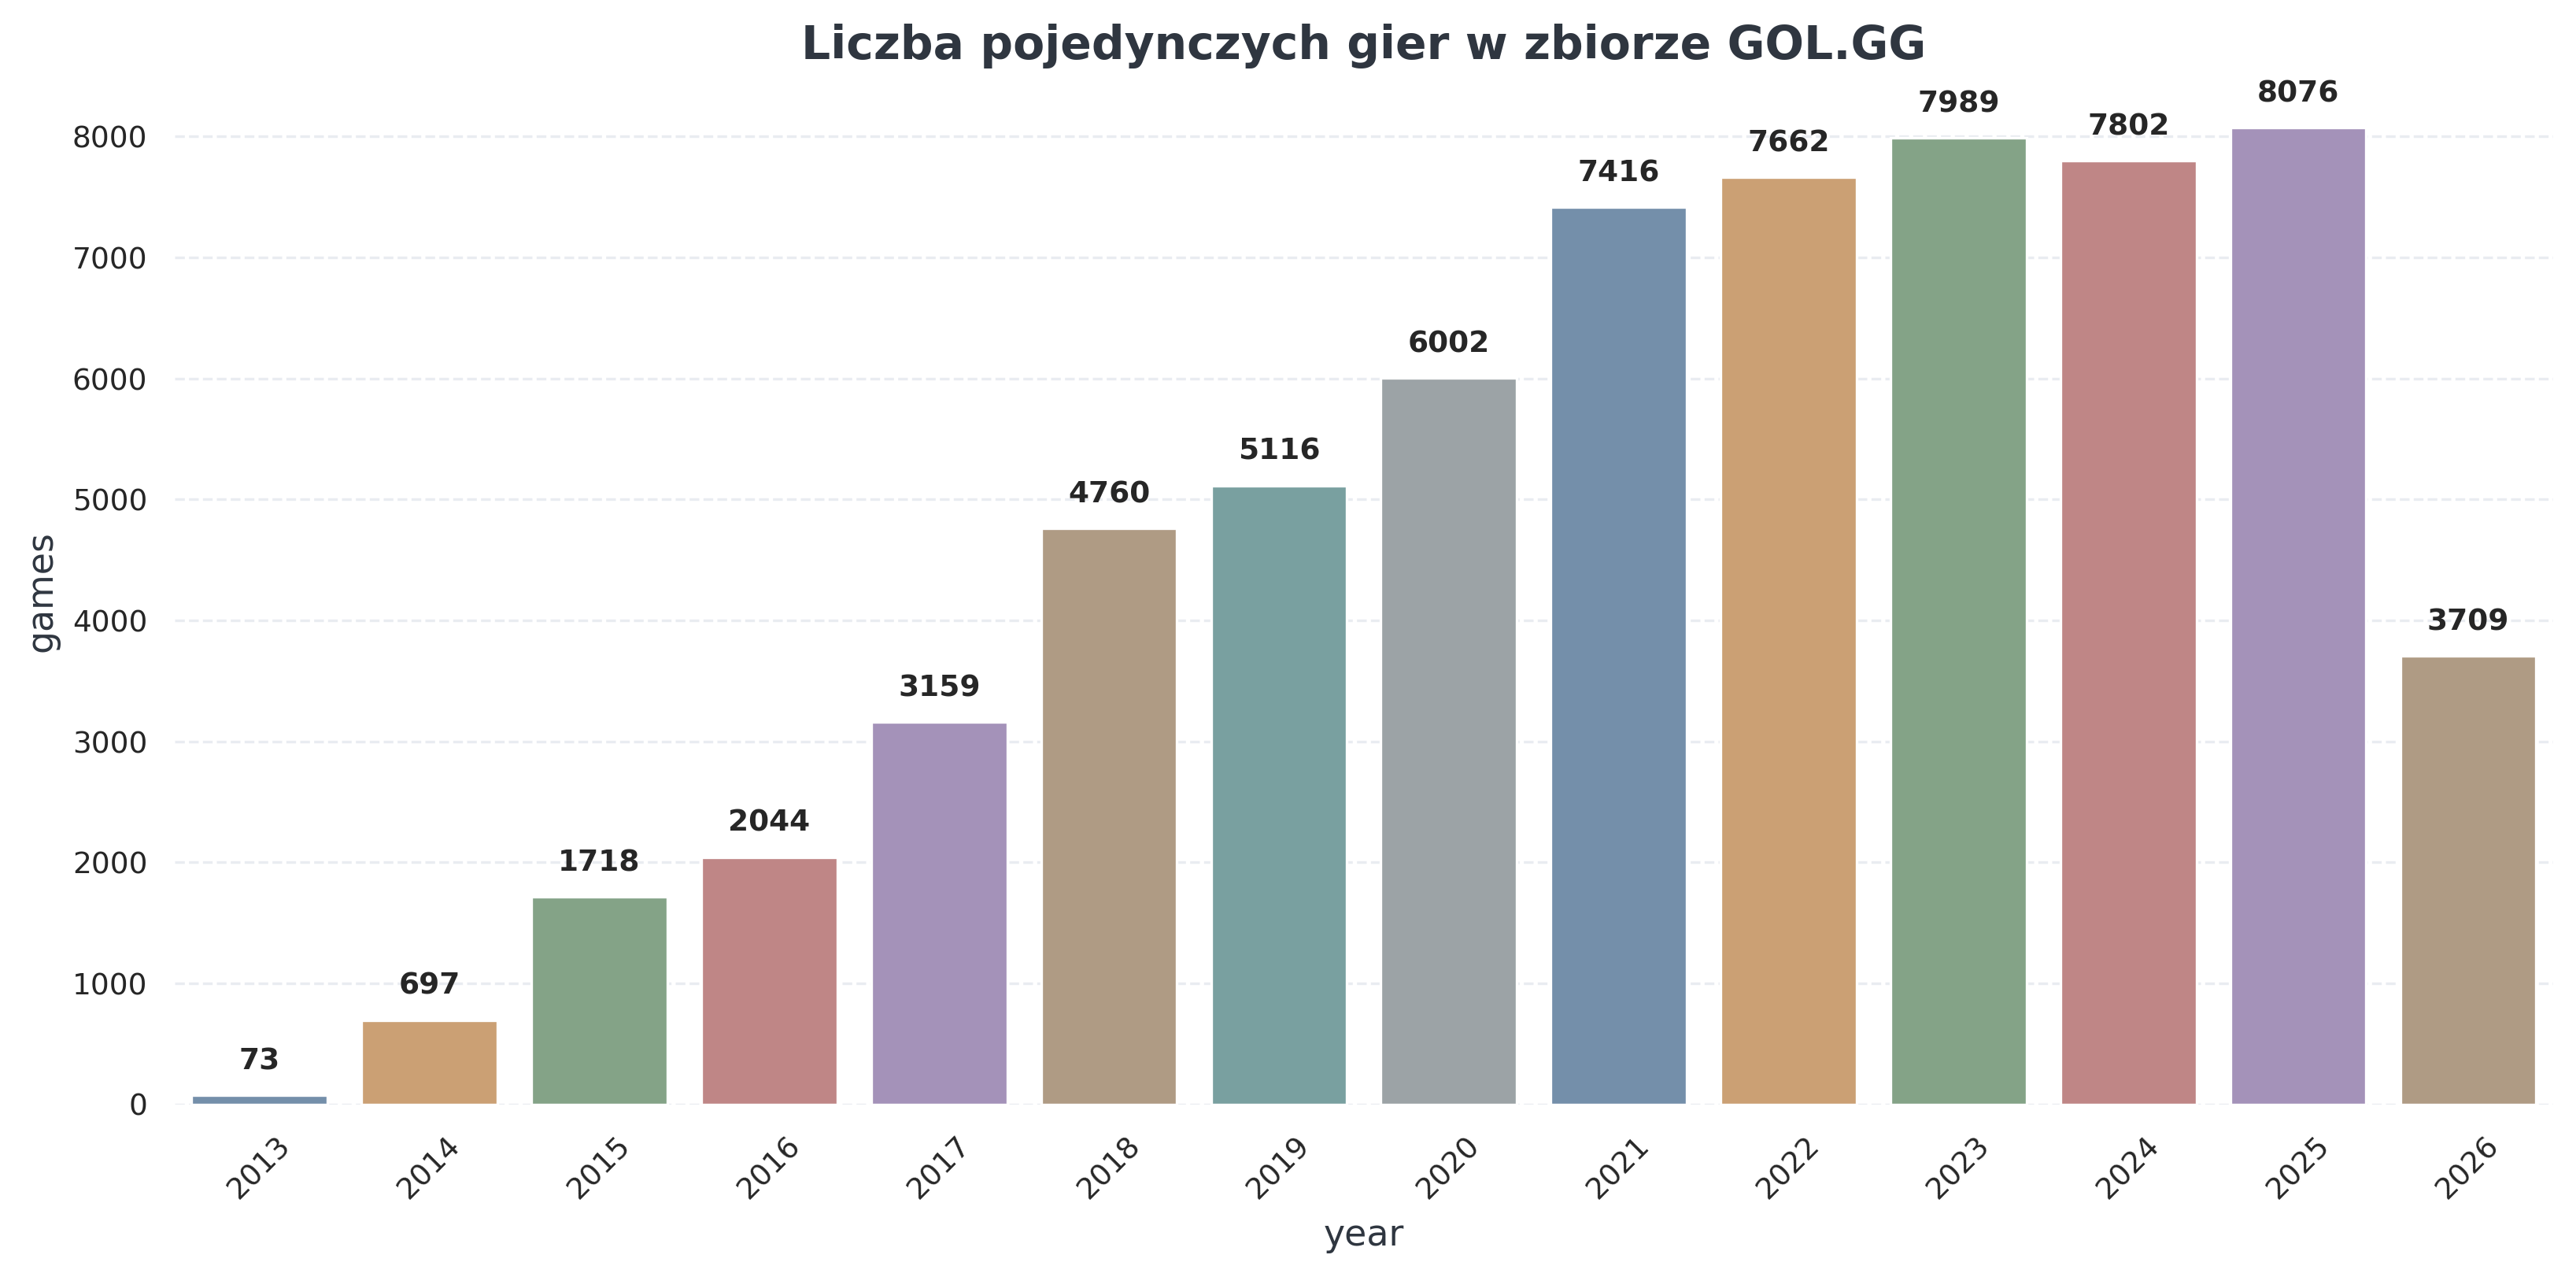
\includegraphics[width=0.9\textwidth]{eda_point4/sport_games_per_year.png}
    \caption{Liczba pojedynczych gier w kolejnych latach w danych GOL.GG.}
    \label{fig:eda_games_per_year}
\end{figure}

Zestawienie \cref{fig:eda_matches_per_year,fig:eda_games_per_year} prowadzi do ważnej obserwacji. Po 2022 roku liczba rekordów meczowych maleje, ale liczba rozegranych gier pozostaje relatywnie wysoka. W aktualnej próbce rok 2025 zawiera mniej meczów niż lata 2021--2024, natomiast liczba pojedynczych gier jest nadal zbliżona do najwyższych wartości w całym szeregu czasowym. Nie oznacza to więc prostego spadku aktywności sceny, lecz zmianę struktury kalendarza i większy udział serii wielomapowych.

\begin{figure}[H]
    \centering
    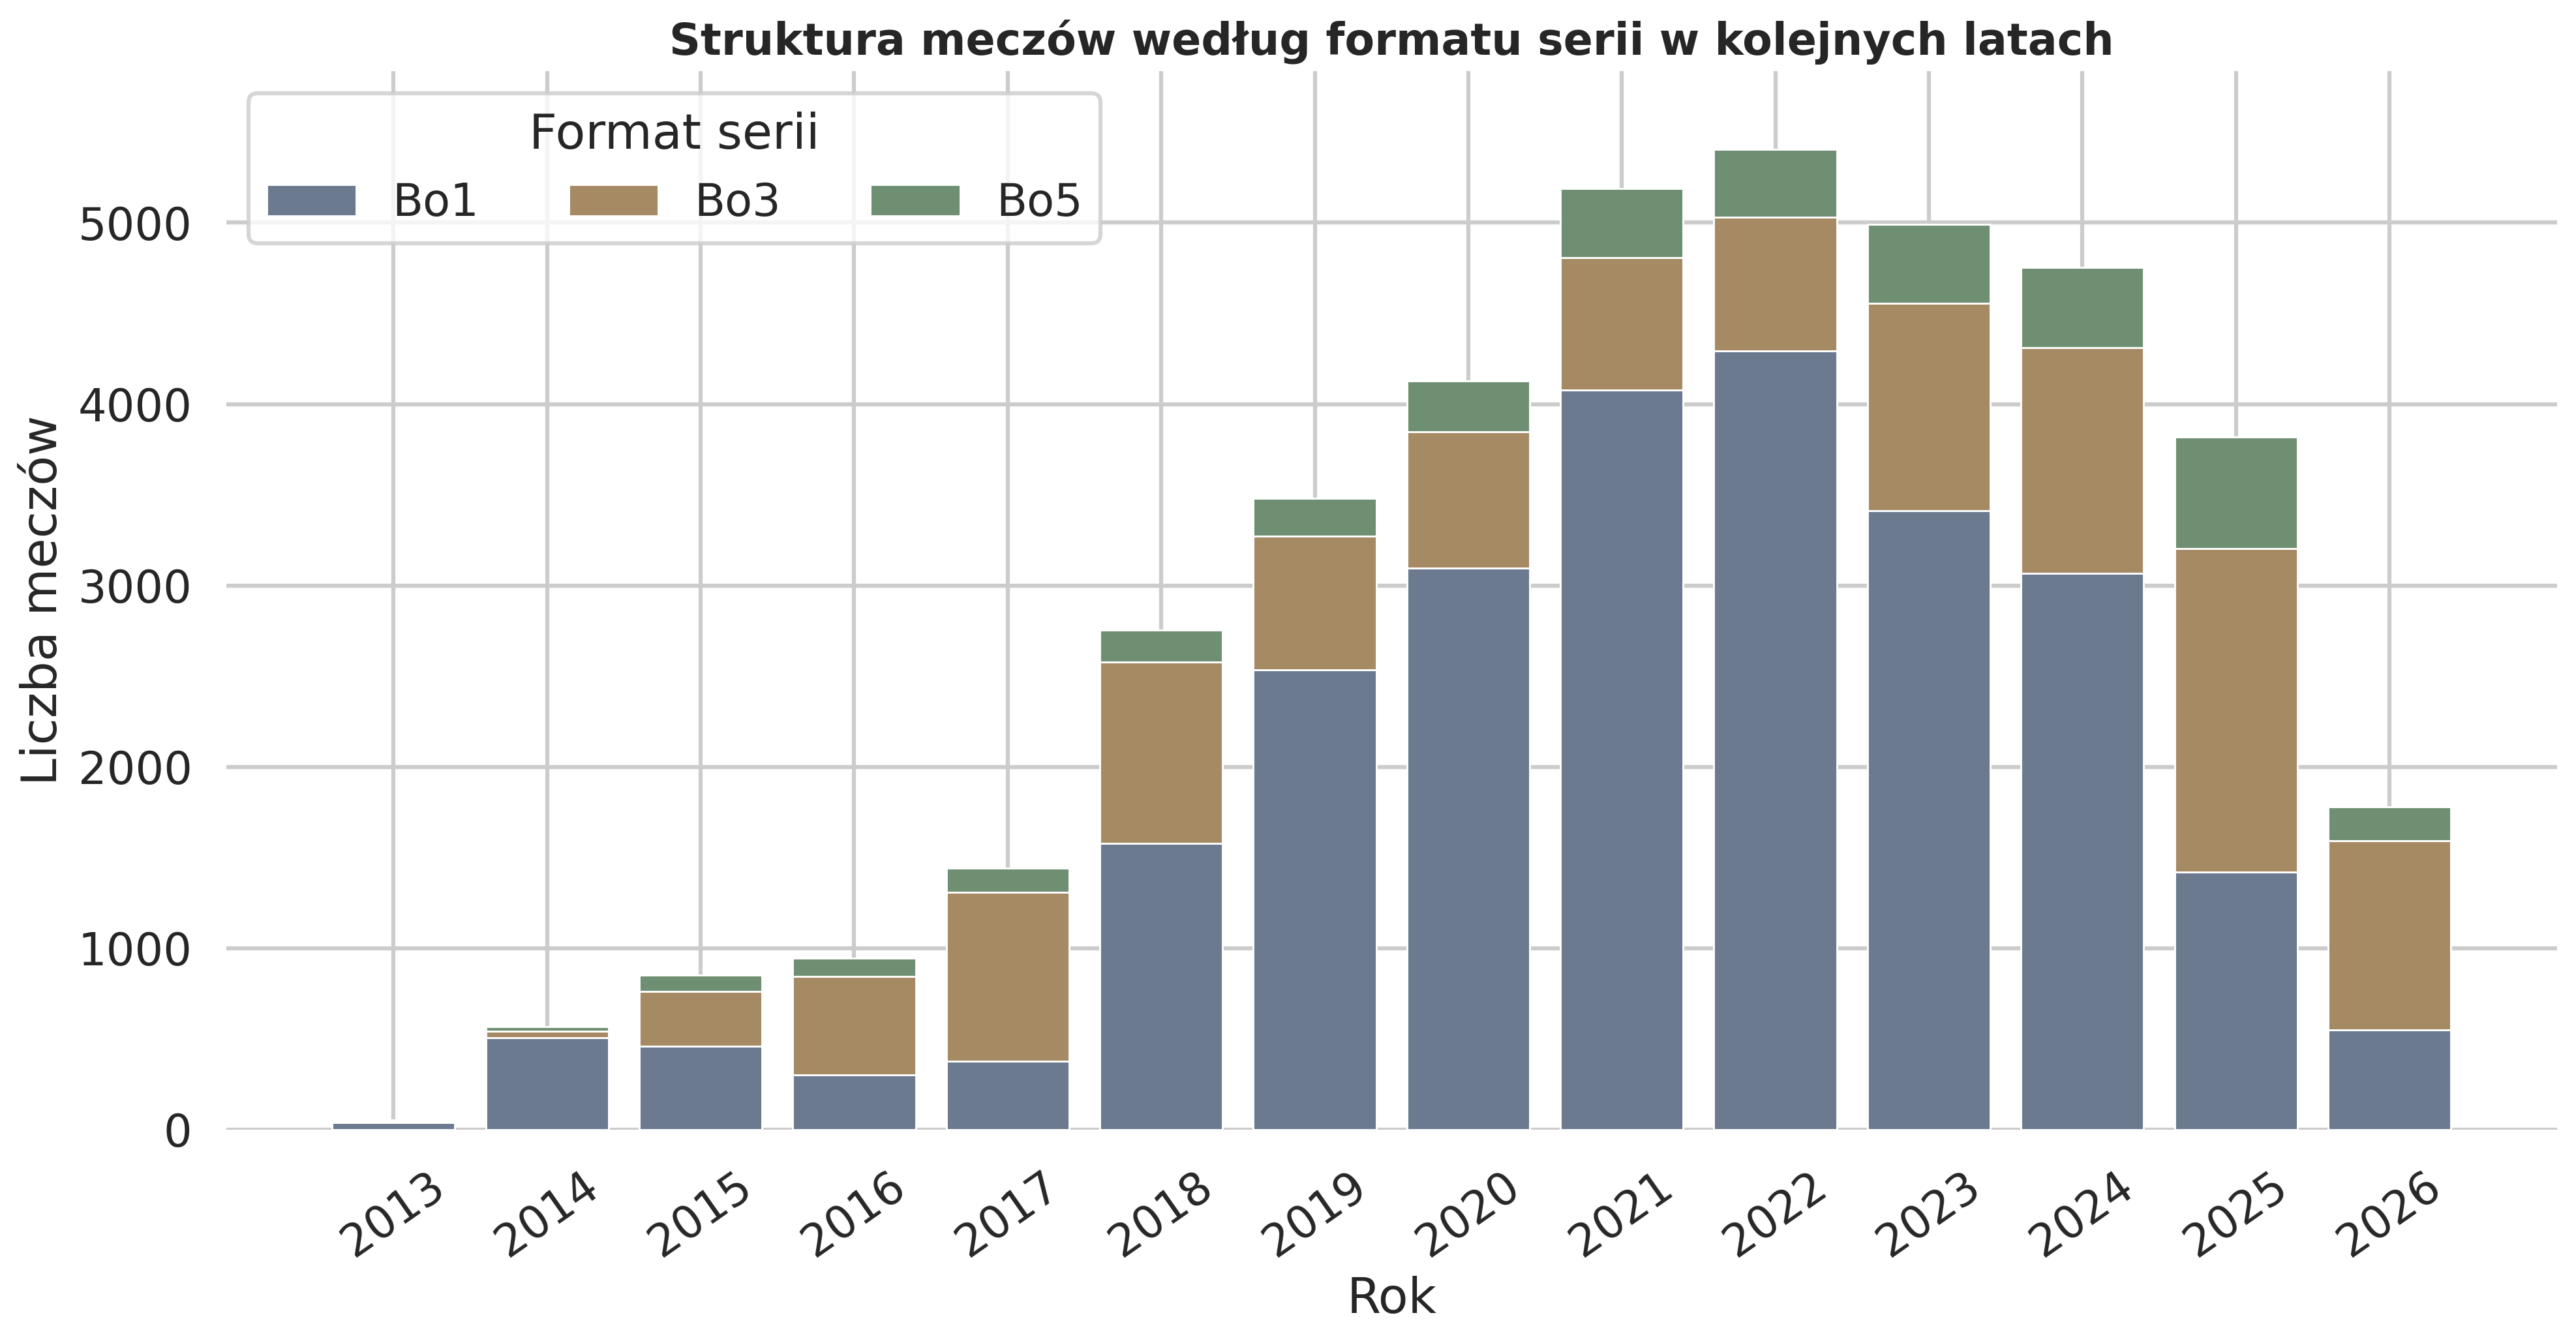
\includegraphics[width=0.95\textwidth]{eda_point4/sport_matches_by_format_per_year_stacked.png}
    \caption{Liczba meczów w kolejnych latach z podziałem według formatu serii.}
    \label{fig:eda_matches_by_format_year}
\end{figure}

Wykres skumulowany na rysunku~\ref{fig:eda_matches_by_format_year} pokazuje, jak zmieniał się udział formatów Bo1, Bo3 i Bo5. Jest to istotne, ponieważ etykieta predykcyjna i kursy bukmacherskie są zdefiniowane na poziomie meczu, natomiast część statystyk sportowych powstaje na poziomie pojedynczych gier. Większy udział Bo3 i Bo5 może więc utrzymywać wysoką liczbę rozegranych map mimo mniejszej liczby rekordów meczowych.

\section{Zmienna objaśniana i balans klas}

Zmienną objaśnianą jest zwycięstwo pierwszej drużyny w uporządkowanej parze meczowej. W idealnym przypadku, przy losowym przypisaniu stron, udział zwycięstw pierwszej drużyny byłby bliski 50\%. W praktyce może występować niewielkie odchylenie od tej wartości, wynikające z konwencji zapisu meczów, kolejności drużyn w źródłach danych lub specyfiki dopasowania danych sportowych do kursów.

Balans klas ma znaczenie dla interpretacji metryk. Sama trafność klasyfikacji przy progu 0{,}5 nie jest wystarczającą miarą jakości, ponieważ model może osiągać pozornie dobre wyniki przez preferowanie częstszej klasy. Dlatego w dalszej części pracy podstawowymi miarami są AUC, LogLoss, Brier score oraz ECE. Metryki te oceniają nie tylko wskazanie zwycięzcy, lecz także jakość przypisanego prawdopodobieństwa.

\begin{figure}[H]
    \centering
    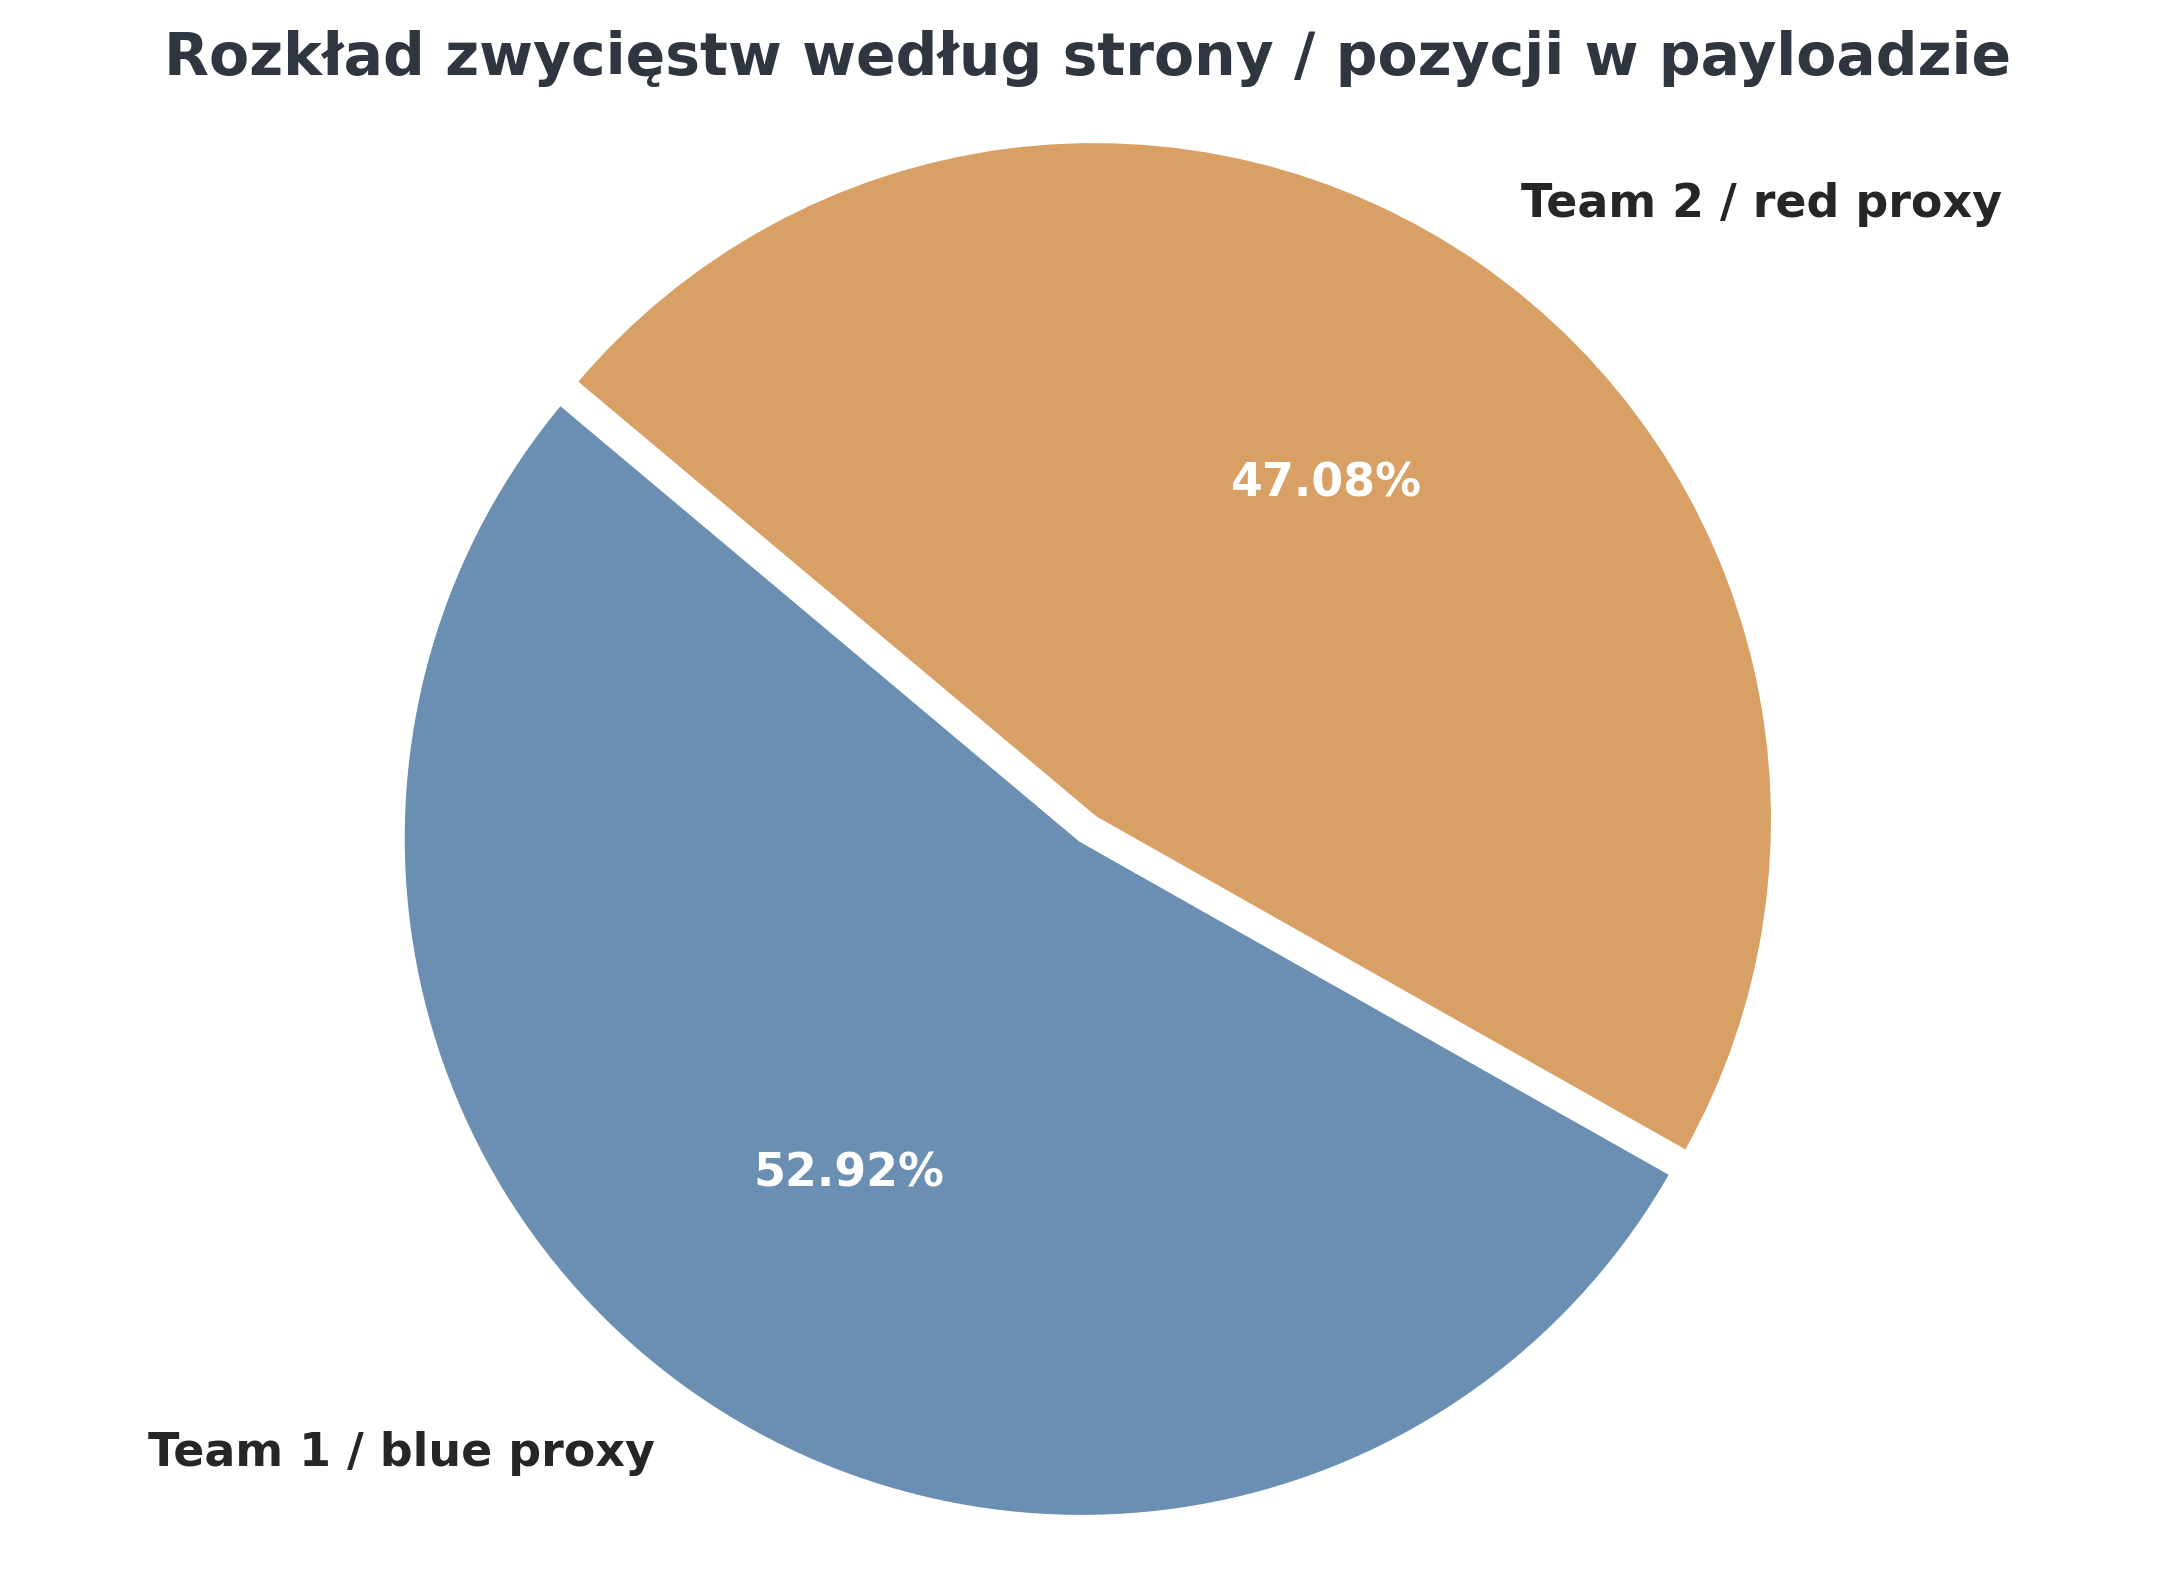
\includegraphics[width=0.75\textwidth]{eda_point4/sport_side_win_rate.png}
    \caption{Udział zwycięstw stron meczu w danych sportowych.}
    \label{fig:eda_side_win_rate}
\end{figure}

Wizualizacja na rysunku~\ref{fig:eda_side_win_rate} pełni funkcję kontroli podstawowej struktury celu predykcyjnego. Jeżeli jedna ze stron byłaby dominująca wyłącznie z powodu sposobu zapisu danych, proste metryki klasyfikacyjne mogłyby być mylące. Z tego powodu w pracy nacisk położono na metryki probabilistyczne.

\section{Formaty meczów}

Profesjonalne mecze \textit{League of Legends} mogą być rozgrywane w różnych formatach serii. Najczęściej spotykane są formaty Bo1, Bo3 oraz Bo5. Różnią się one nie tylko liczbą gier potrzebnych do rozstrzygnięcia meczu, lecz także poziomem losowości wyniku.

W formacie Bo1 pojedyncza gra decyduje o wyniku całego meczu. Taki format jest bardziej podatny na jednorazowe błędy, nietypowe strategie lub specyficzne przygotowanie do konkretnego przeciwnika. W formacie Bo3 drużyna musi wygrać dwie gry, co częściowo redukuje wpływ pojedynczego zdarzenia. Format Bo5 jest zwykle stosowany w fazach pucharowych i finałach, przez co obejmuje specyficzną grupę meczów o wysokiej stawce.

Segmentacja według formatu jest istotna, ponieważ model może działać z różną skutecznością w zależności od typu serii. W późniejszej ewaluacji najlepsze wyniki osiągane są w formacie Bo3, natomiast format Bo5 okazuje się trudniejszy do oceny. Wynika to prawdopodobnie z mniejszej liczby obserwacji oraz specyfiki meczów play-off, w których mierzą się silniejsze i bardziej wyrównane drużyny.

\begin{figure}[H]
    \centering
    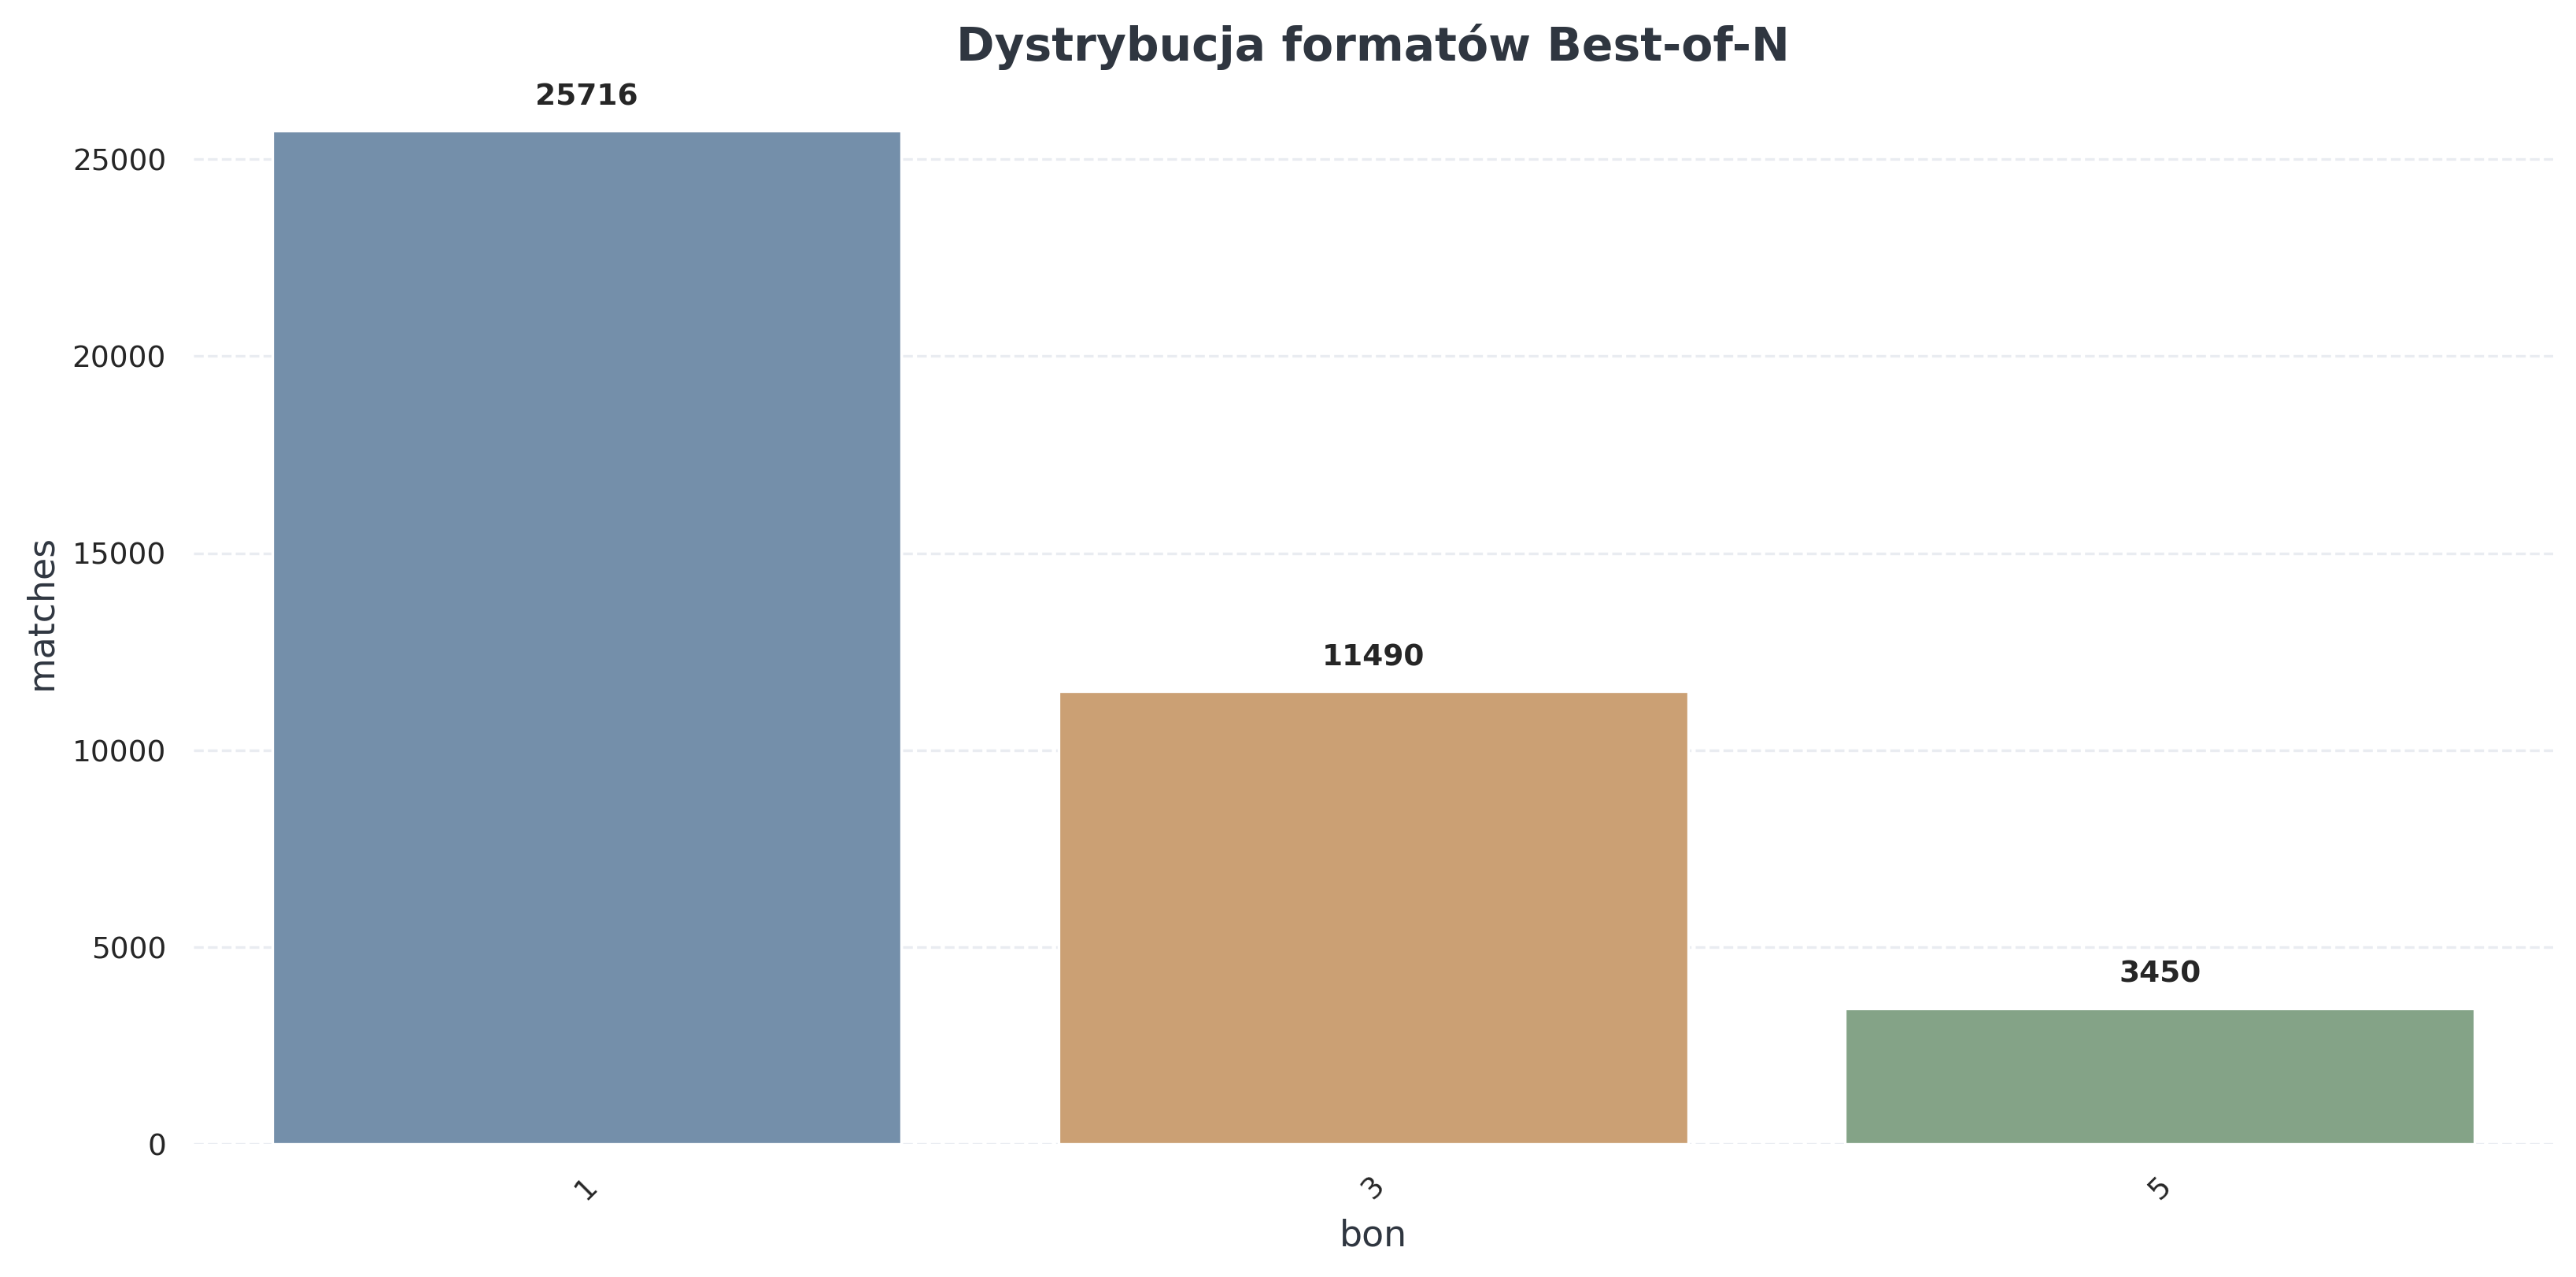
\includegraphics[width=0.9\textwidth]{eda_point4/sport_bon_distribution.png}
    \caption{Rozkład formatów serii w danych sportowych.}
    \label{fig:eda_bon_distribution}
\end{figure}

Rozkład przedstawiony na rysunku~\ref{fig:eda_bon_distribution} uzasadnia raportowanie wyników w segmentach Bo1, Bo3 i Bo5. Segmenty te różnią się liczebnością i charakterem sportowym, dlatego końcowa ocena modelu nie powinna ograniczać się wyłącznie do jednej zagregowanej metryki.

\section{Poziom rozgrywek}

Drugim wymiarem segmentacji jest poziom rozgrywek. Stabilność składów, dostępność informacji i efektywność rynku mogą różnić się między ligami najwyższego poziomu a rozgrywkami regionalnymi. Segmentacja służy tu kontroli struktury próby, a nie budowie osobnych modeli dla każdego poziomu.

Ponieważ GOL.GG nie zawiera jawnej zmiennej poziomu rozgrywek, zastosowano operacyjny podział na Tier 1 i Tier 2. Tier 1 obejmuje turnieje międzynarodowe najwyższego poziomu oraz główne ligi LCK, LPL, LEC i LCS, natomiast Tier 2 pozostałe rozgrywki regionalne, ligi akademickie i challengers. Jest to heurystyka oparta na nazwie turnieju, a nie oficjalna klasyfikacja Riot Games.

\begin{figure}[H]
    \centering
    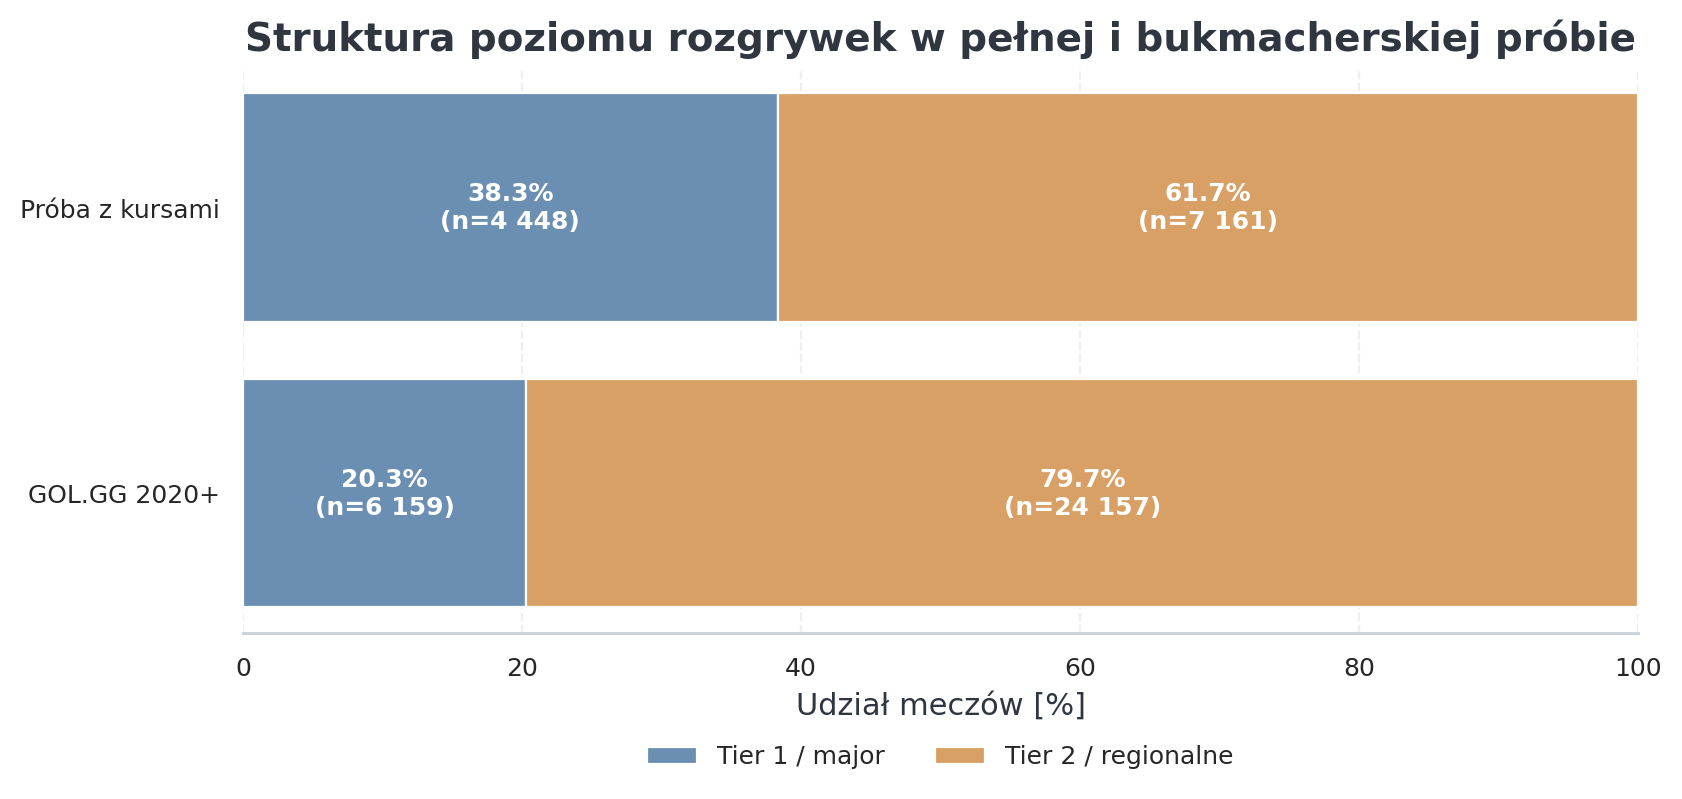
\includegraphics[width=0.88\textwidth]{eda_point4/tier_coverage_common_sample.png}
    \caption{Udział meczów Tier 1 i Tier 2 w pełnej próbie sportowej od 2020 roku oraz we wspólnej próbie z kursami bukmacherskimi.}
    \label{fig:eda_tier_coverage_common_sample}
\end{figure}

\begin{table}[H]
    \centering
    \caption{Struktura poziomu rozgrywek w danych sportowych i w próbie bukmacherskiej}
    \label{tab:eda_tier_coverage_common_sample}
    \begin{tabular}{llrr}
        \toprule
        Próba & Segment & Liczba meczów & Udział [\%] \\
        \midrule
        GOL.GG 2020+ & Tier 1 / major & 6~159 & 20{,}3 \\
        GOL.GG 2020+ & Tier 2 / regionalne & 24~157 & 79{,}7 \\
        Próba z kursami & Tier 1 / major & 4~448 & 38{,}3 \\
        Próba z kursami & Tier 2 / regionalne & 7~161 & 61{,}7 \\
        \bottomrule
    \end{tabular}
\end{table}

\Cref{fig:eda_tier_coverage_common_sample,tab:eda_tier_coverage_common_sample} pokazują, że wspólna próba z kursami nie jest zdominowana wyłącznie przez niszowe rozgrywki. W porównaniu z pełną historią sportową od 2020 roku ma ona wyższy udział meczów Tier 1: około 38{,}3\% wobec 20{,}3\%. Jednocześnie nadal zawiera dużą część rozgrywek Tier 2, co oznacza, że końcowa ewaluacja obejmuje zarówno najbardziej rozpoznawalne ligi i turnieje, jak i segment regionalny. 
Taka struktura jest korzystna dla celu pracy: rynek bukmacherski dostarcza benchmark głównie tam, gdzie mecz jest wystarczająco istotny, aby zostać wyceniony, ale próba nie redukuje się wyłącznie do jednego wąskiego poziomu rozgrywek.

\section{Rynek bukmacherski jako punkt odniesienia}

Kursy bukmacherskie są silnym benchmarkiem, ponieważ agregują informacje o drużynach, składach, formie i reakcji rynku. W pracy rozróżniono kursy otwarcia, bliższe realistycznej predykcji przedmeczowej, oraz kursy zamknięcia, traktowane jako silniejszy benchmark diagnostyczny.

Na wspólnej próbce historycznej rynek otwarcia osiąga wyniki wyraźnie lepsze od losowego klasyfikatora, co potwierdza, że kursy zawierają istotną informację predykcyjną. Rynek zamknięcia jest zwykle silniejszy od rynku otwarcia, co jest zgodne z intuicją: im bliżej meczu, tym więcej informacji może zostać uwzględnionych w cenie.

\begin{figure}[H]
    \centering
    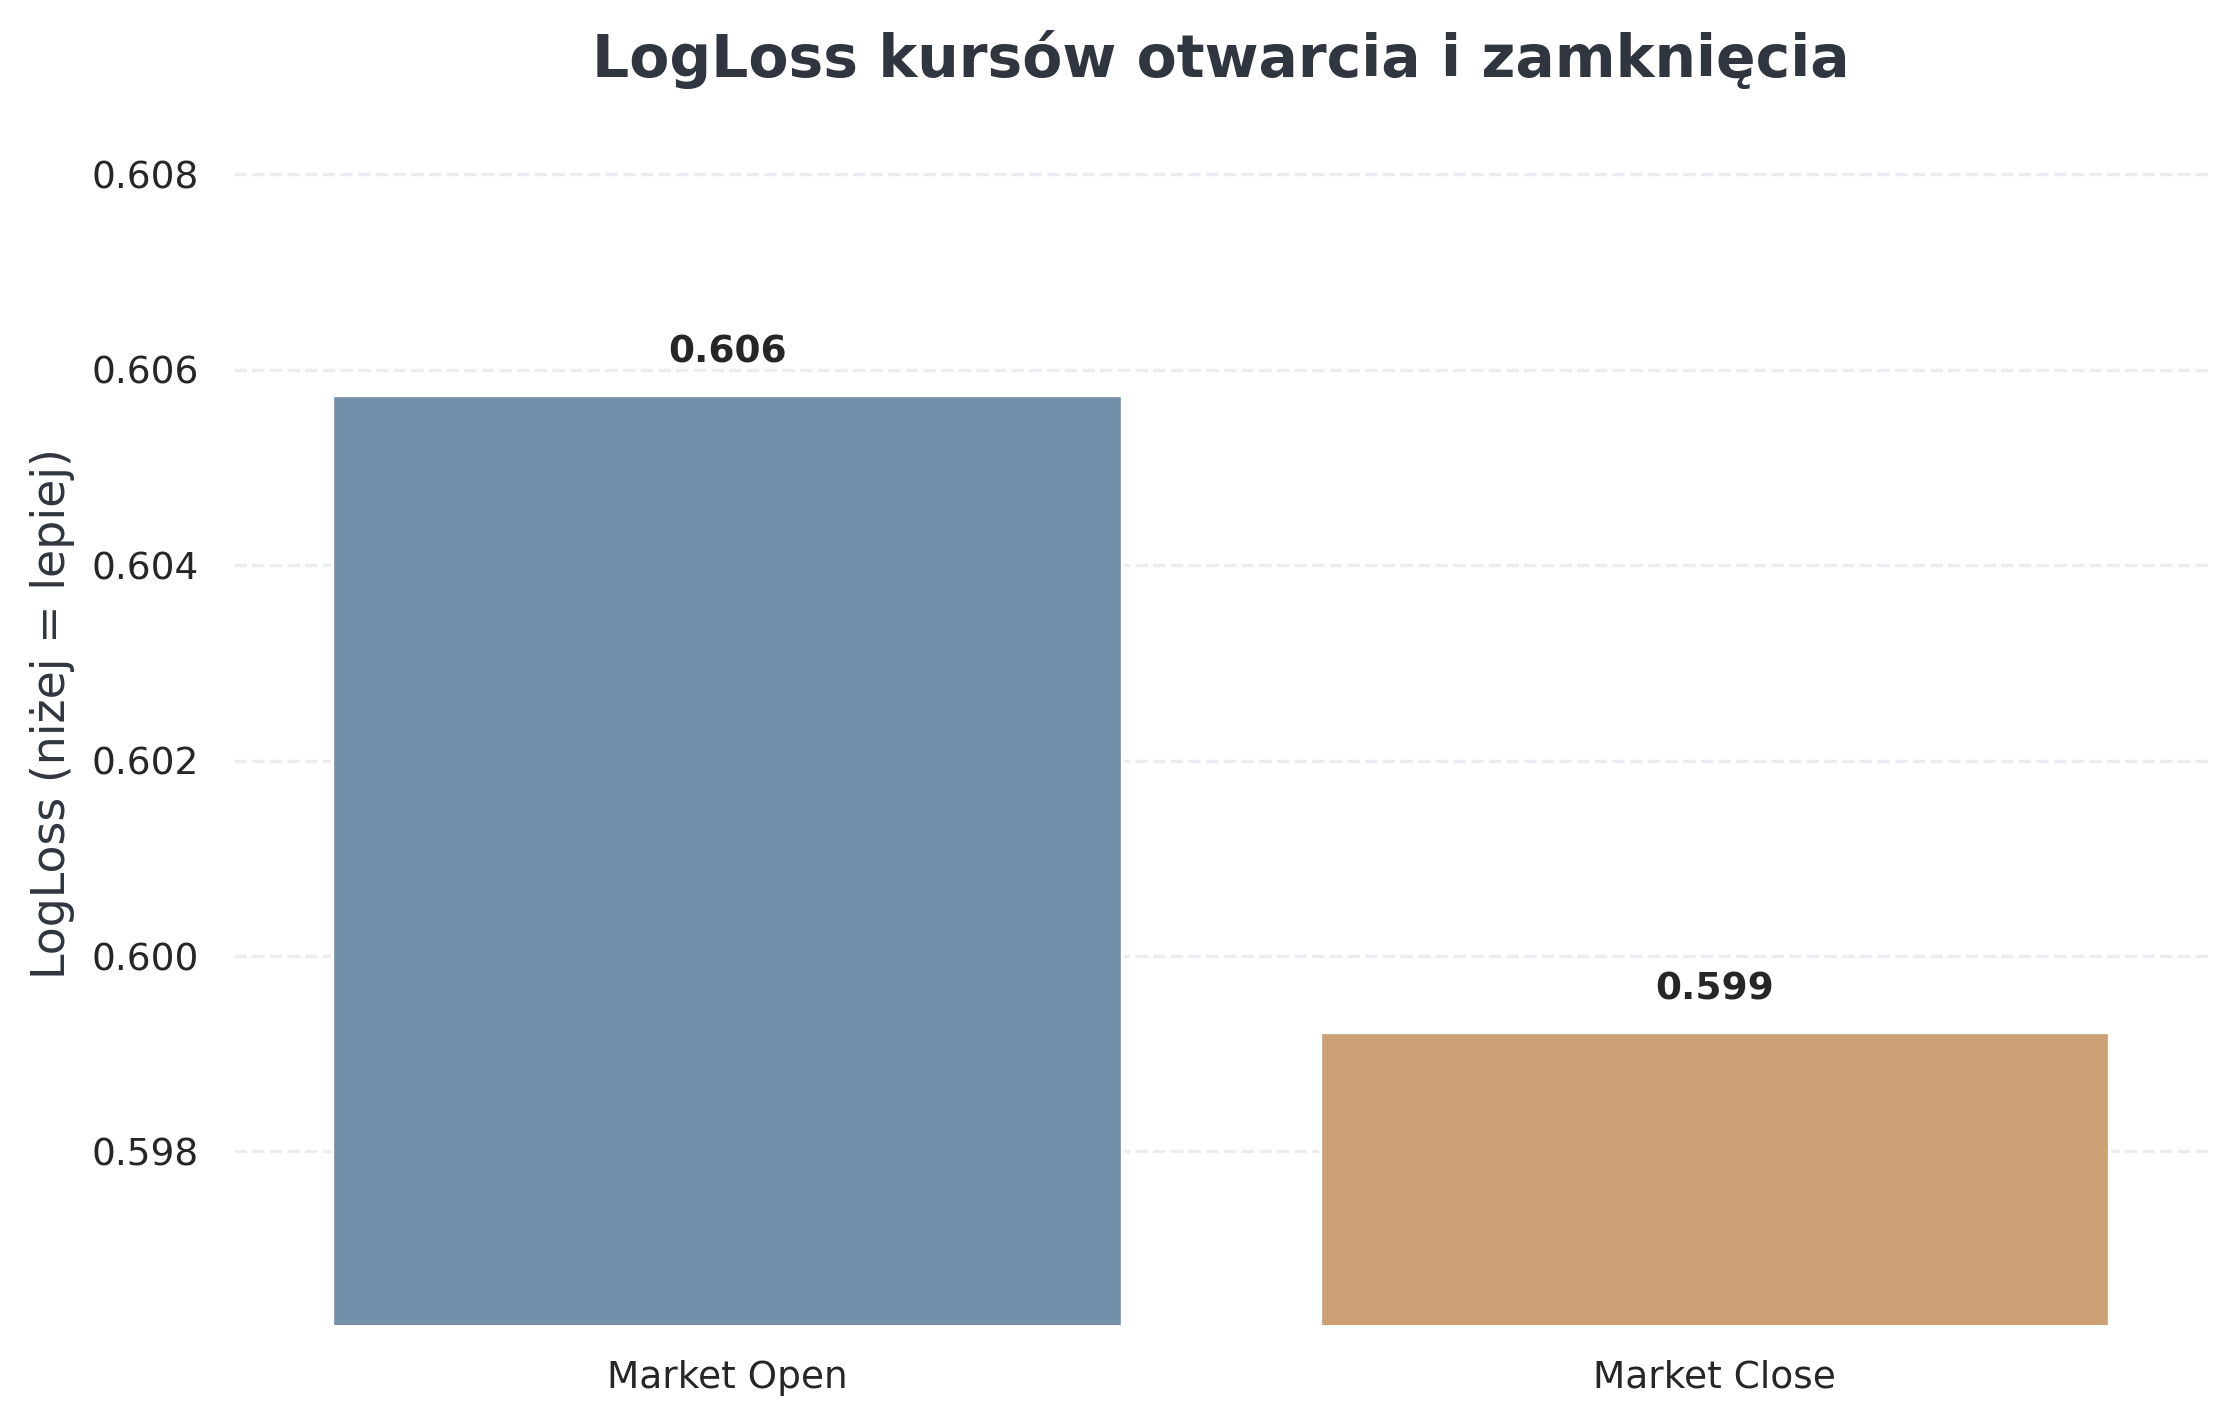
\includegraphics[width=0.85\textwidth]{eda_point4/market_auc_overall.png}
    \caption{Porównanie jakości kursów otwarcia i zamknięcia jako benchmarku probabilistycznego.}
    \label{fig:eda_market_auc_overall}
\end{figure}

\begin{table}[H]
    \centering
    \caption{Orientacyjne wyniki benchmarku bukmacherskiego na wspólnej próbce historycznej}
    \label{tab:eda_market_benchmark}
    \begin{tabular}{lrr}
        \toprule
        Benchmark & AUC & LogLoss \\
        \midrule
        Market Open & 0{,}7325 & 0{,}6057 \\
        Market Close & 0{,}7403 & 0{,}5992 \\
        \bottomrule
    \end{tabular}
\end{table}

Wyniki w tabeli~\ref{tab:eda_market_benchmark} nie są jeszcze końcową oceną modelu. Pokazują natomiast, że rynek jest wymagającym punktem odniesienia, a kurs zamknięcia jest silniejszy od kursu otwarcia.

Jakość benchmarku bukmacherskiego nie musi być jednak taka sama dla każdego formatu serii. W formacie Bo1 pojedyncza gra decyduje o wyniku meczu, natomiast w Bo3 i Bo5 wynik całej serii zależy od kilku gier. Z tego powodu dodatkowo sprawdzono, jak LogLoss kursów otwarcia i zamknięcia zmienia się pomiędzy segmentami Bo1, Bo3 i Bo5.

\begin{figure}[H]
    \centering
    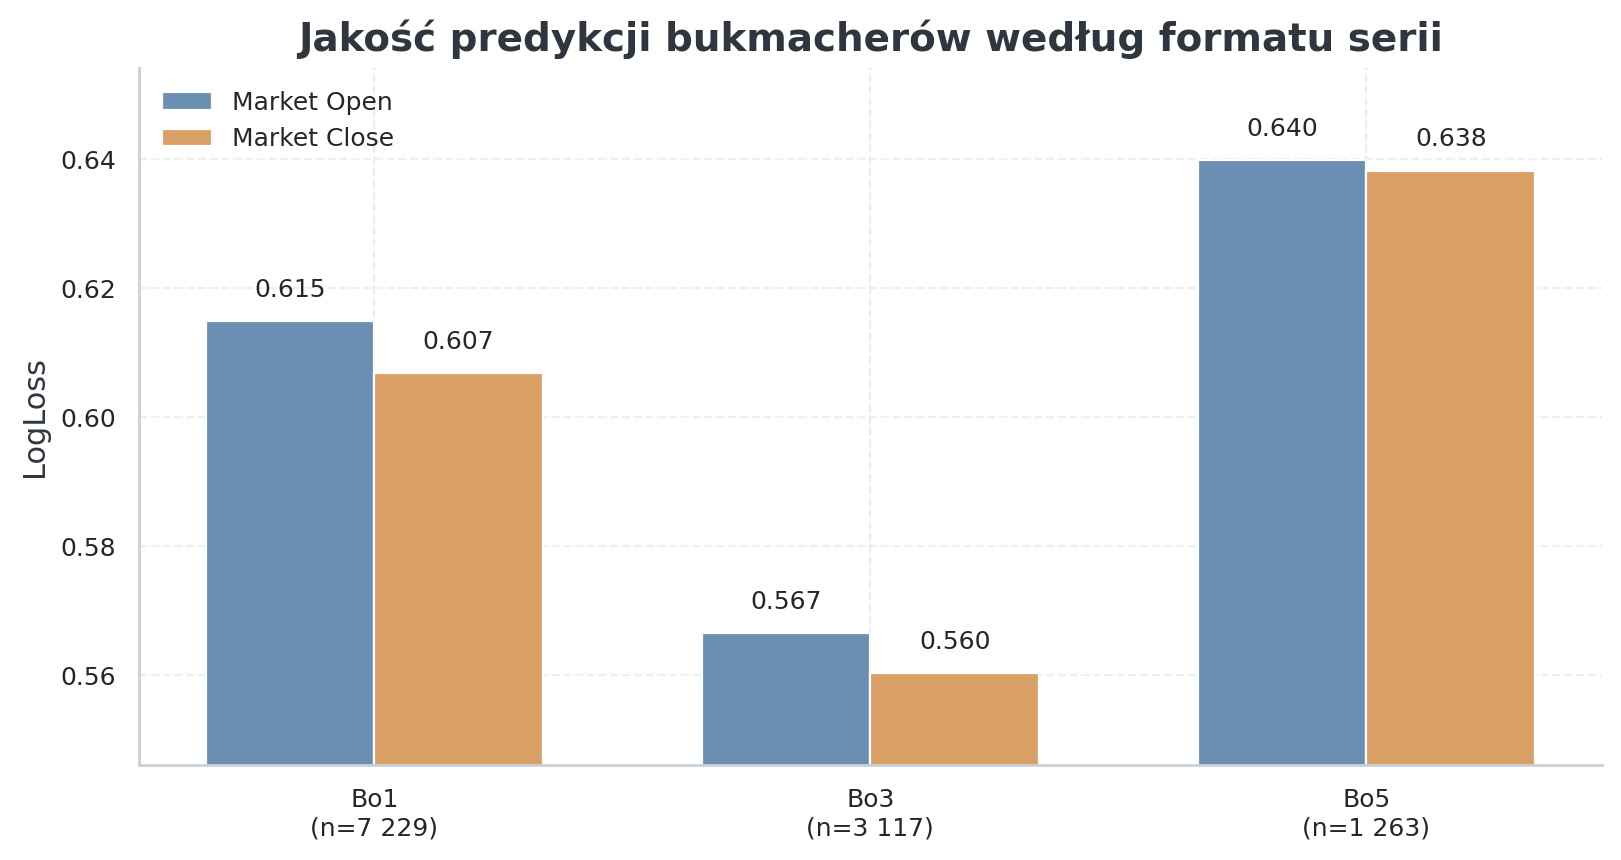
\includegraphics[width=0.86\textwidth]{eda_point4/market_quality_by_bon_logloss.png}
    \caption{Jakość predykcji bukmacherów według formatu serii na wspólnej próbie z kursami. Niższy LogLoss oznacza lepszą jakość probabilistyczną.}
    \label{fig:eda_market_quality_by_bon}
\end{figure}

\begin{table}[H]
    \centering
    \caption{Jakość benchmarku bukmacherskiego według formatu serii}
    \label{tab:eda_market_quality_by_bon}
    \begin{tabular}{llrrrr}
        \toprule
        Format & Benchmark & Mecze & AUC & LogLoss & ECE \\
        \midrule
        Bo1 & Market Open & 7~229 & 0{,}7206 & 0{,}6150 & 0{,}0139 \\
        Bo1 & Market Close & 7~229 & 0{,}7312 & 0{,}6068 & 0{,}0114 \\
        Bo3 & Market Open & 3~117 & 0{,}7784 & 0{,}5665 & 0{,}0213 \\
        Bo3 & Market Close & 3~117 & 0{,}7840 & 0{,}5604 & 0{,}0153 \\
        Bo5 & Market Open & 1~263 & 0{,}6682 & 0{,}6398 & 0{,}0544 \\
        Bo5 & Market Close & 1~263 & 0{,}6742 & 0{,}6382 & 0{,}0486 \\
        \bottomrule
    \end{tabular}
\end{table}

\Cref{fig:eda_market_quality_by_bon,tab:eda_market_quality_by_bon} pokazują, że rynek najlepiej radził sobie w segmencie Bo3. Dla kursu zamknięcia LogLoss wyniósł tam około 0{,}5604, wobec 0{,}6068 dla Bo1 i 0{,}6382 dla Bo5. Słabszy wynik Bo5 należy interpretować ostrożnie: segment jest mniejszy i obejmuje głównie mecze play-off oraz spotkania silnych drużyn. Analiza uzasadnia uwzględnienie formatu serii w cechach modelu.

Oprócz jakości predykcyjnej ważna jest marża kursów. Dla rynku dwuwynikowego można ją przybliżyć jako nadwyżkę sumy odwrotności kursów ponad jeden. W analizowanej próbce średnia marża kursów otwarcia wynosiła około 8{,}17\%, a średnia ważona liczbą meczów około 8{,}29\%. Dlatego surowe kursy wymagały normalizacji, a w tabeli~\ref{tab:bookmaker_margin_summary} zestawiono jednocześnie pokrycie, marżę, AUC i LogLoss.

\begin{figure}[H]
    \centering
    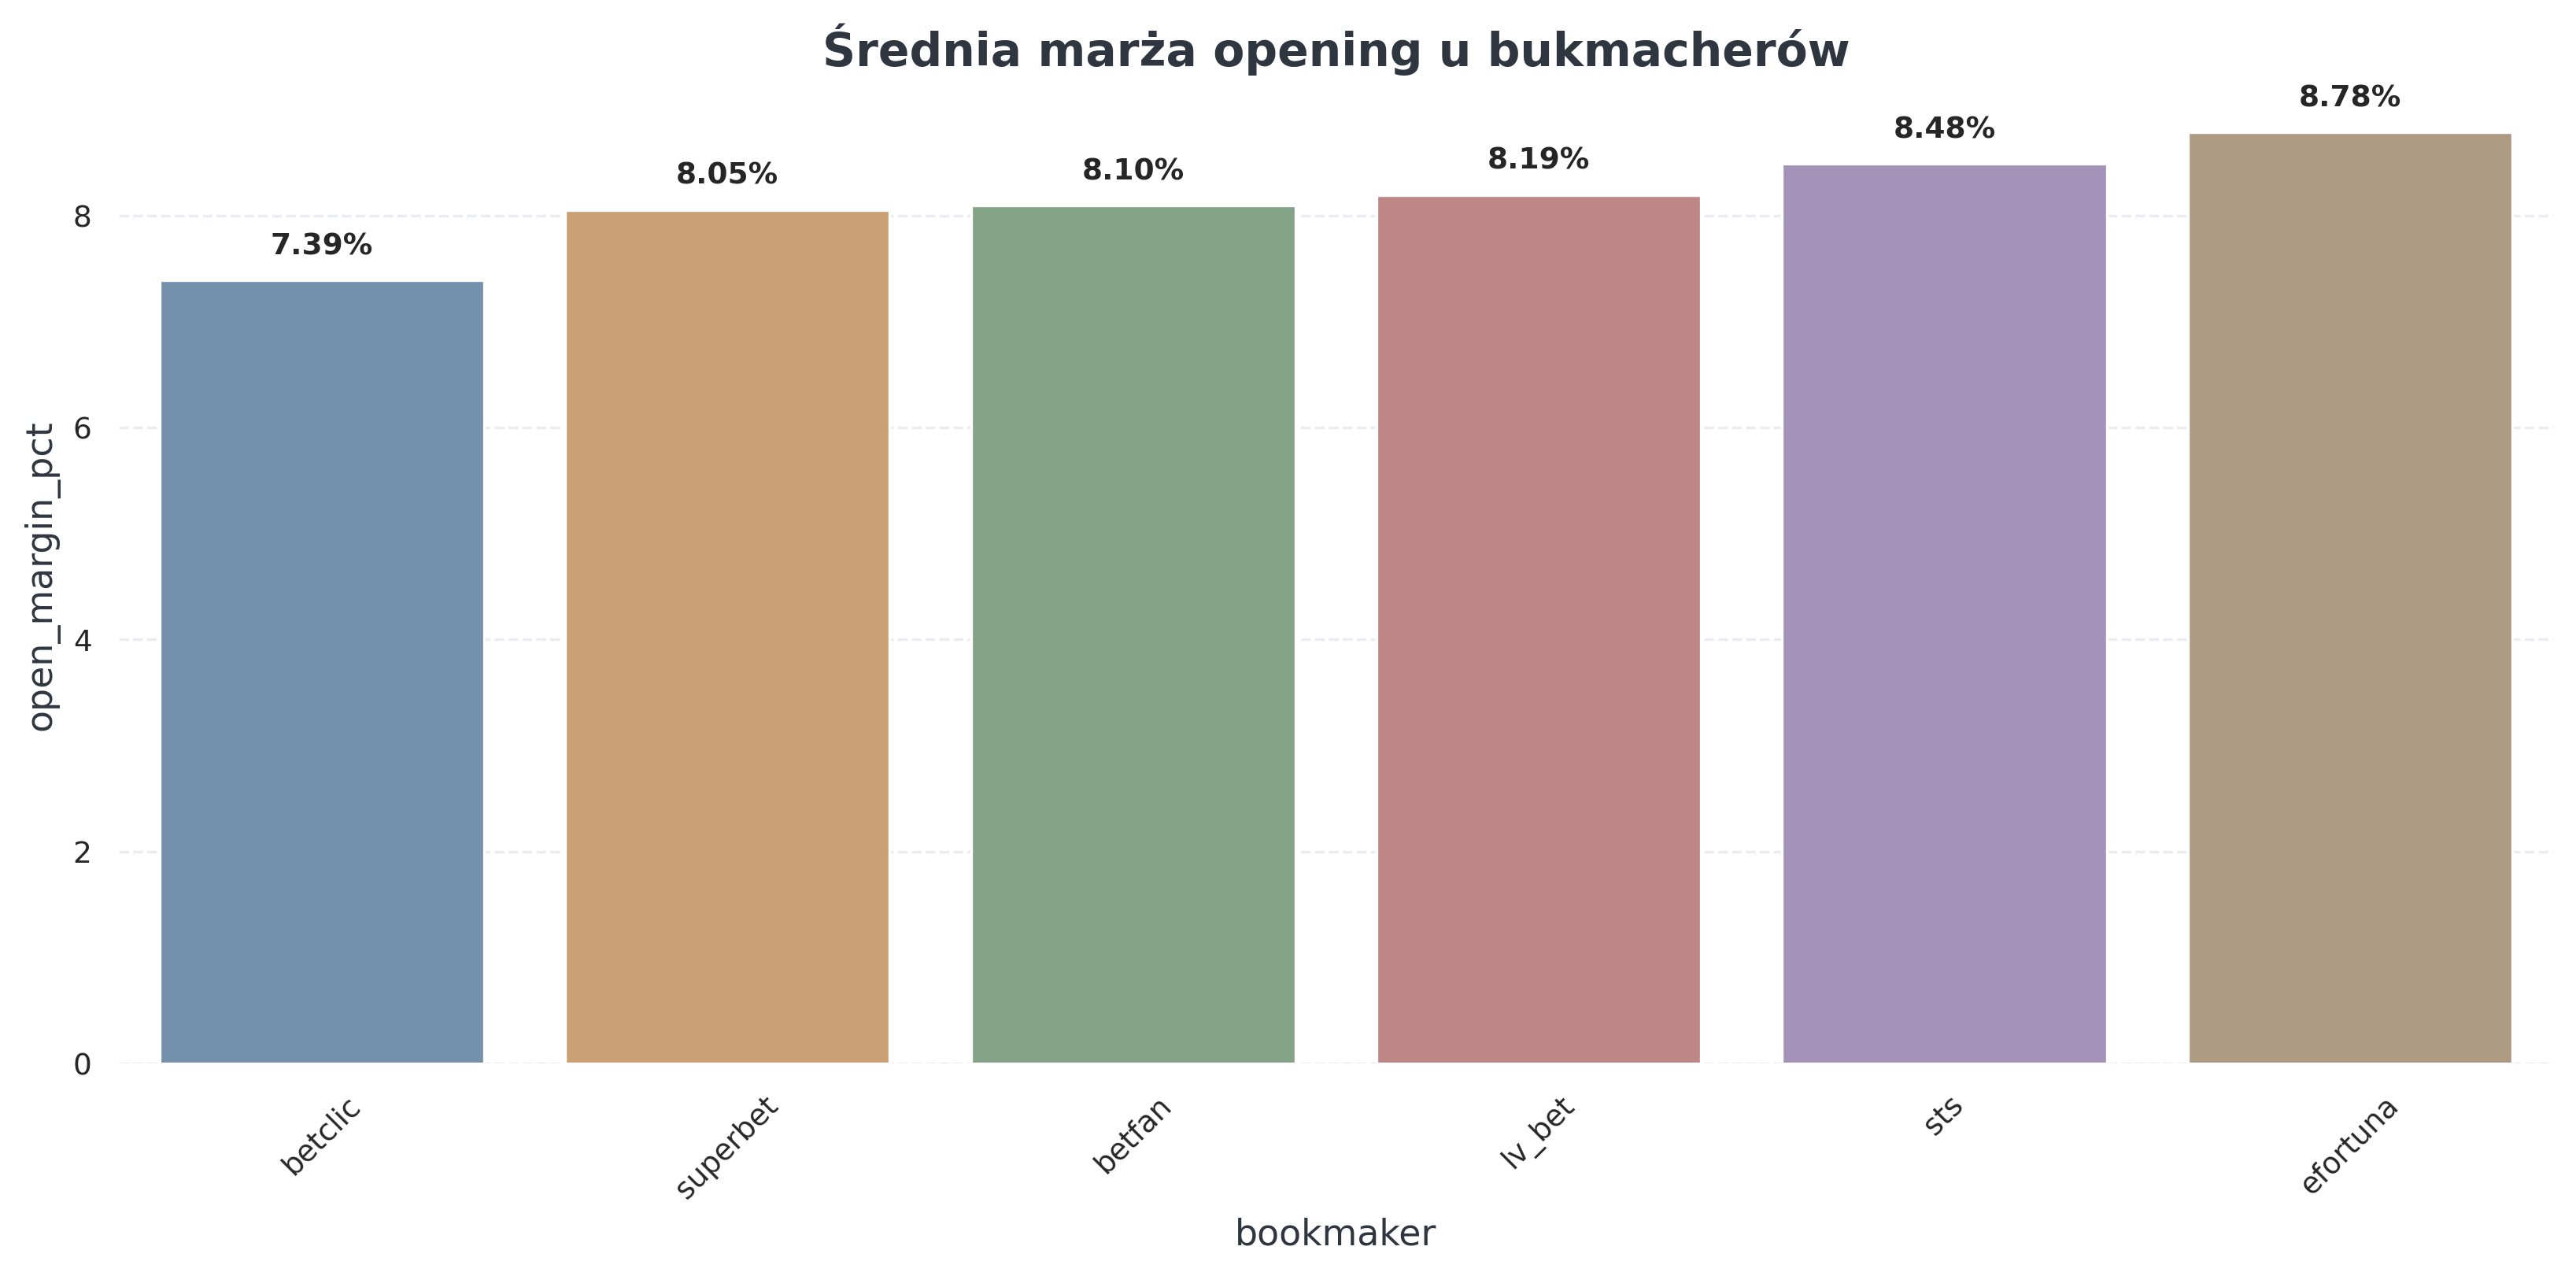
\includegraphics[width=0.9\textwidth]{eda_point4/market_bookmaker_margins.png}
    \caption{Średnia marża kursów otwarcia według bukmachera.}
    \label{fig:eda_bookmaker_margins}
\end{figure}

\begin{table}[H]
    \centering
    \caption{Pokrycie danych, marża i jakość predykcyjna kursów otwarcia według bukmachera}
    \label{tab:bookmaker_margin_summary}
    \resizebox{\textwidth}{!}{%
    \begin{tabular}{lrrrrr}
        \toprule
        Bukmacher & Mecze z kursem otwarcia & Pokrycie [\%] & Marża [\%] & AUC & LogLoss \\
        \midrule
        Betclic & 4~153 & 25{,}36 & 7{,}39 & 0{,}7418 & 0{,}5980 \\
        Superbet & 9~444 & 57{,}67 & 8{,}05 & 0{,}7255 & 0{,}6111 \\
        Betfan & 11~404 & 69{,}64 & 8{,}10 & 0{,}7298 & 0{,}6077 \\
        LV BET & 13~159 & 80{,}36 & 8{,}19 & 0{,}7323 & 0{,}6061 \\
        STS & 13~695 & 83{,}63 & 8{,}48 & 0{,}7299 & 0{,}6079 \\
        eFortuna & 13~902 & 84{,}90 & 8{,}78 & 0{,}7307 & 0{,}6069 \\
        \midrule
        Średnia rynkowa & 16~308 & 99{,}59 & 8{,}29 & 0{,}7325 & 0{,}6057 \\
        \bottomrule
    \end{tabular}
    }
\end{table}

Betclic miał najniższą marżę i najlepszy LogLoss wśród pojedynczych bukmacherów, ale obejmował tylko około jedną czwartą próby. Największe pokrycie miały eFortuna, STS i LV BET. Średnia rynkowa obejmuje prawie całą próbę, dlatego jest stabilniejszym benchmarkiem niż pojedynczy operator.

\section{Historyczne statystyki gry jako źródło kontekstu}

Dane GOL.GG zawierają także informacje opisujące przebieg poszczególnych gier, między innymi statystyki zawodników i drużyn. Część takich zmiennych, na przykład przewaga w złocie w piętnastej minucie aktualnej gry, jest silnie związana z końcowym wynikiem. Nie może być jednak użyta bezpośrednio w predykcji przedmeczowej, ponieważ w momencie predykcji aktualna gra jeszcze się nie odbyła.

Jedną z takich zmiennych jest GD@15, czyli \textit{gold difference at 15 minutes}. Oznacza ona różnicę w łącznej liczbie złota zgromadzonego przez obie drużyny w 15. minucie gry. Dodatnia wartość GD@15 dla drużyny oznacza, że po pierwszych 15 minutach miała ona przewagę ekonomiczną nad przeciwnikiem, natomiast wartość ujemna oznacza stratę. W praktyce jest to syntetyczna miara jakości wczesnej fazy gry, ponieważ złoto odzwierciedla zabójstwa, farmę, kontrolę mapy i zdobyte cele.

W predykcji przedmeczowej nie można użyć GD@15 z aktualnej gry, ponieważ ta wartość jest znana dopiero po rozpoczęciu meczu. Można natomiast obliczyć historyczne GD@15 drużyny, czyli średnią przewagę lub stratę w złocie w 15. minucie w jej wcześniejszych grach. 
Taka zmienna opisuje, czy dana drużyna zwykle dobrze rozpoczynała swoje mecze i czy potrafiła budować przewagę ekonomiczną we wczesnej fazie gry.

Z tego powodu w pracy wykorzystano wyłącznie historyczne agregaty takich informacji. Przykładowo, zamiast używać przewagi w złocie z aktualnej gry, obliczono średnią przewagę w złocie z wcześniejszych występów drużyny. Następnie dla każdego meczu wyznaczono różnicę tych średnich wartości pomiędzy Team 1 i Team 2. 
Taka cecha opisuje wcześniejszy styl oraz formę zespołu przed meczem, a jednocześnie nie narusza zasady chronologicznego dostępu do informacji.

Formalnie, dla meczu rozgrywanego w chwili \(t\), historyczna cecha Team 1 może być zapisana jako średnia z wcześniejszych gier tej drużyny:

\begin{equation}
    \overline{GD@15}_{Team1,t} = \frac{1}{K}\sum_{k=1}^{K} GD@15_{Team1,t-k},
\end{equation}

gdzie \(K\) oznacza liczbę wcześniejszych gier uwzględnionych w oknie historycznym. W analizie eksploracyjnej i późniejszych modelach najważniejsza jest różnica pomiędzy analogicznymi wartościami dla obu drużyn:

\begin{equation}
    \Delta GD@15_t = \overline{GD@15}_{Team1,t} - \overline{GD@15}_{Team2,t}.
\end{equation}

Dodatnia wartość \(\Delta GD@15_t\) oznacza, że Team 1 miał historycznie lepszą wczesną fazę gry niż Team 2, natomiast wartość ujemna oznacza przewagę Team 2 w tym aspekcie.

Ta obserwacja uzasadnia późniejsze wprowadzenie metamodelu z kontekstem historycznym. Same ratingi opisują ogólną siłę zawodników i drużyn, ale cechy kroczące mogą dostarczyć dodatkowej informacji o aktualnej formie, dynamice gry oraz niedawnych wynikach.

Zależność pomiędzy historyczną przewagą GD@15 a wynikiem meczu można ocenić bez używania informacji z aktualnej gry. Dla czytelności analizę ograniczono do części próby z lat 2024--2026, dla której dostępne były kursy bukmacherskie. Pominięto również mecze, w których różnica historycznego GD@15 była równa zero, ponieważ nie wskazywały one przewagi żadnej ze stron. W tak zdefiniowanej próbie Team 1 wygrywał około 65{,}2\% meczów, gdy jego historyczne GD@15 było wyższe od rywala, oraz około 42{,}5\% meczów, gdy było niższe. Oznacza to, że historyczny profil early game był powiązany z późniejszym wynikiem meczu.

Siłę tej zależności sprawdzono również prostą diagnostyką jednowymiarową. Korelacja Pearsona pomiędzy różnicą historycznego GD@15 a wynikiem meczu wyniosła około 0{,}252, a korelacja rang Spearmana około 0{,}259. Jednowymiarowa regresja logistyczna oparta wyłącznie na tej zmiennej uzyskała AUC równe 0{,}650 i LogLoss równy 0{,}656. Wynik ten jest zbyt słaby, aby traktować historyczne GD@15 jako samodzielny model predykcyjny, ale wystarczająco wyraźny, aby uzasadnić pozostawienie tej zmiennej jako składnika szerszego kontekstu historycznego.

Tę samą zmienną można następnie przedstawić w sposób zagregowany, dzieląc mecze na przedziały różnicy historycznego GD@15 i obliczając rzeczywisty udział zwycięstw Team 1 w każdym przedziale. Taka wizualizacja bezpośrednio pokazuje, czy historyczna przewaga wczesnej fazy gry była powiązana z późniejszym wynikiem meczu.

\begin{figure}[H]
    \centering
    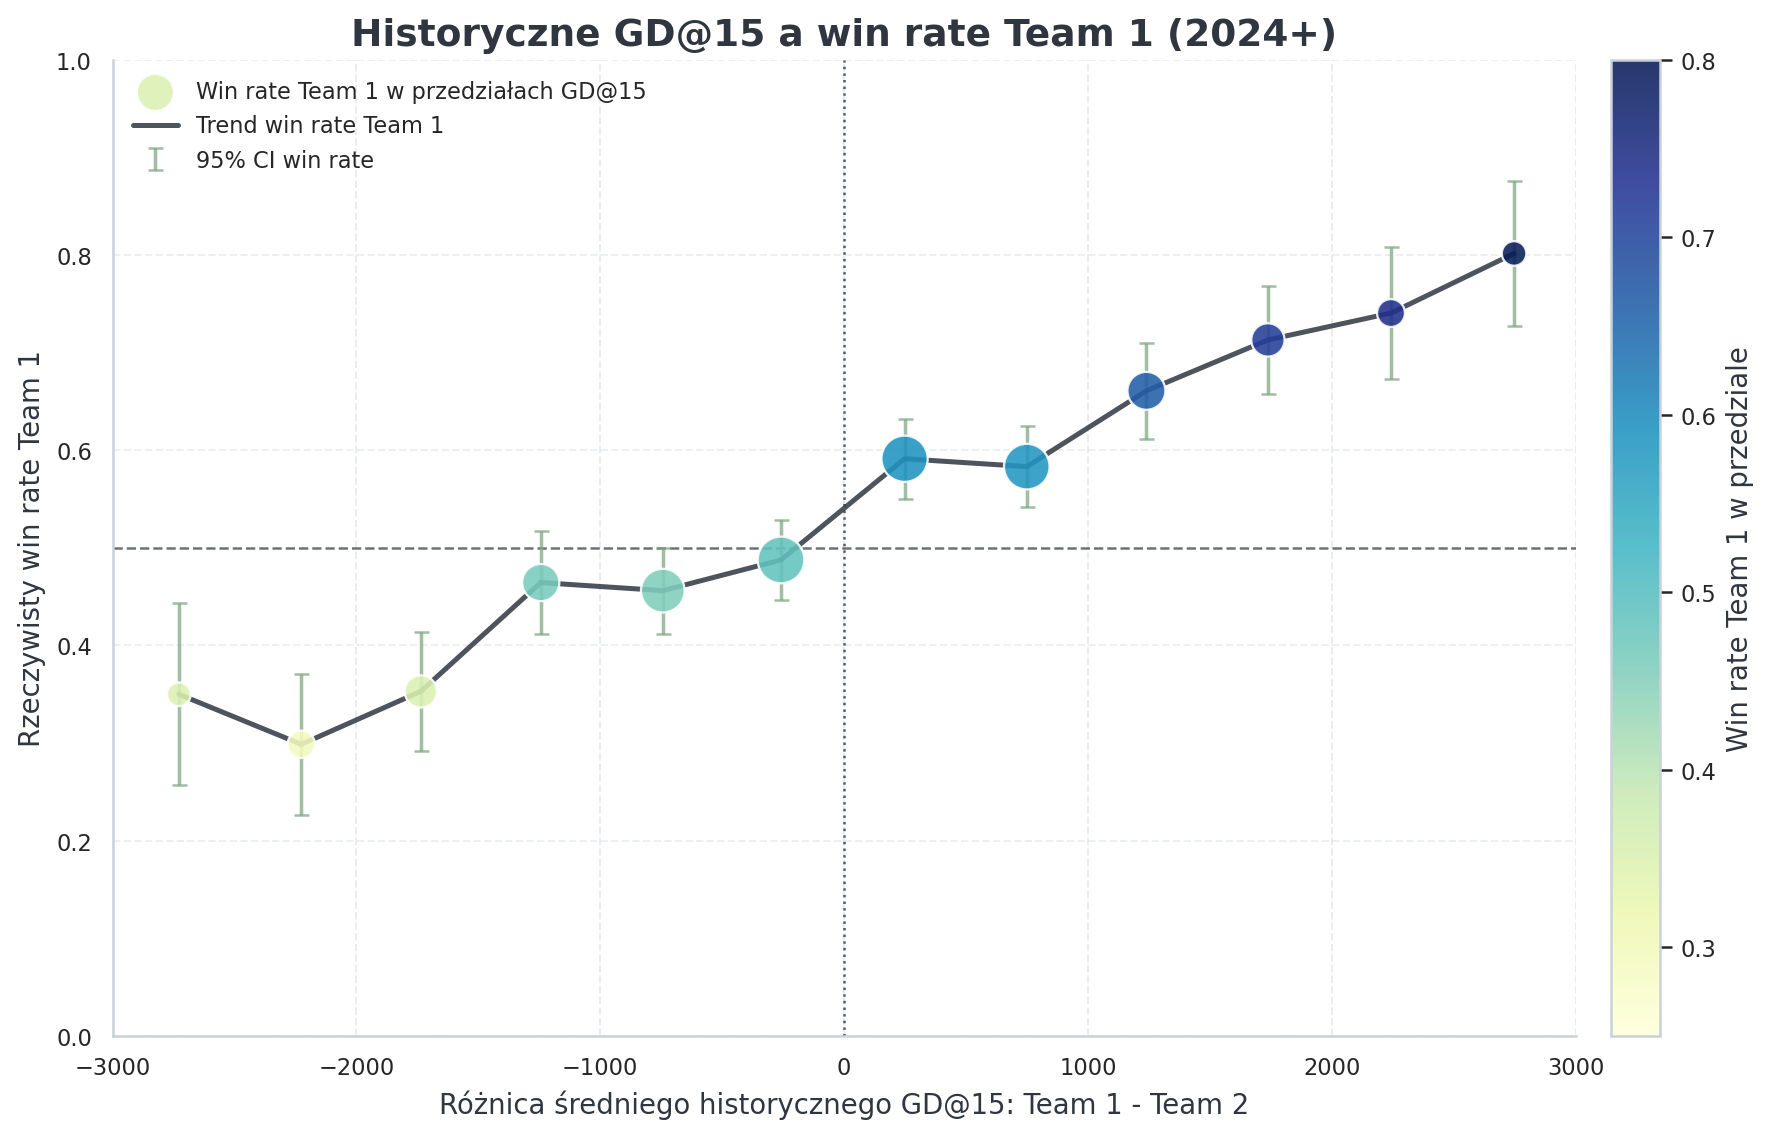
\includegraphics[width=0.90\textwidth]{eda_point4/historical_gd15_diff_vs_winrate.png}
    \caption{Relacja pomiędzy różnicą średniego historycznego GD@15 a rzeczywistym win rate Team 1.}
    \label{fig:eda_historical_gd15_market_open}
\end{figure}

\Cref{fig:eda_historical_gd15_market_open} pokazuje tę zależność w formie wykresu punktowego po przedziałach GD@15. Każdy punkt oznacza przedział różnicy historycznego GD@15, jego położenie na osi pionowej odpowiada rzeczywistemu win rate Team 1, a wielkość punktu informuje o liczbie meczów w danym przedziale. Wraz ze wzrostem historycznej przewagi GD@15 rośnie rzeczywisty udział zwycięstw Team 1. Oznacza to, że historyczna siła drużyn w early game pozostaje użytecznym kandydatem do modelu kontekstowego, mimo że nie wykorzystuje informacji z aktualnego meczu.

\section{Obserwacje nietypowe i konsekwencje dla modelowania}

Analiza eksploracyjna ujawniła kilka cech próby istotnych dla interpretacji wyników. Po pierwsze, liczba meczów i liczba pojedynczych gier nie zawsze zmieniają się równolegle, ponieważ formaty Bo3 i Bo5 generują więcej map na jeden rekord meczowy. Po drugie, Bo5 jest mniejszym i specyficznym segmentem play-off, dlatego jego wyniki należy interpretować ostrożnie. Po trzecie, mecze z bardzo wysokimi kursami mogą silnie wpływać na LogLoss, co wzmacnia znaczenie metryk probabilistycznych. Po czwarte, Market Open i Market Close pełnią różne role: pierwszy jest wcześniejszym punktem odniesienia, drugi silniejszym benchmarkiem diagnostycznym.

\section{Wnioski z analizy eksploracyjnej}

Z EDA wynikają trzy decyzje metodologiczne. Po pierwsze, predykcja musi być oceniana chronologicznie. Po drugie, format meczu i poziom rozgrywek powinny być analizowane jako segmenty próby. Po trzecie, pełna historia sportowa służy do budowy ratingów i cech historycznych, natomiast wspólna próbka z kursami służy do końcowego porównania z rynkiem.

\chapter{Metodyka oceny modeli}

\section{Cel rozdziału}

Celem tego rozdziału jest określenie zasad, według których oceniane są systemy rankingowe, metamodel oraz benchmark bukmacherski. Jest to istotne, ponieważ badany problem nie polega wyłącznie na wskazaniu zwycięzcy meczu, lecz na oszacowaniu prawdopodobieństwa zwycięstwa jednej ze stron. Z tego względu metryki powinny oceniać jakość predykcji probabilistycznej, a nie tylko decyzję klasyfikacyjną po przyjęciu arbitralnego progu.

W pracy przyjęto, że każdy model zwraca wartość \(\hat{p}_i \in (0,1)\), interpretowaną jako prawdopodobieństwo zwycięstwa pierwszej strony meczu w obserwacji \(i\). Rzeczywisty wynik oznaczono jako \(y_i \in \{0,1\}\), gdzie \(1\) oznacza zwycięstwo pierwszej strony, a \(0\) zwycięstwo drugiej strony.

\section{Wspólna próba ewaluacyjna}

Główna ewaluacja modeli w pracy jest prowadzona na wspólnej próbie meczów, dla których dostępne są zarówno dane sportowe z GOL.GG, jak i historyczne kursy bukmacherskie pochodzące z OddsPortal. Takie ograniczenie próby pozwala porównywać modele sportowe z benchmarkiem rynkowym w tych samych warunkach. Dzięki temu różnice w metrykach nie wynikają z odmiennego zakresu danych, lecz z jakości analizowanych predykcji.

Pełniejsza historia sportowa może być używana do budowy rankingów i historycznych cech kontekstowych, ponieważ w realistycznym scenariuszu predykcyjnym wcześniejsze wyniki zespołów i zawodników są znane przed meczem. Końcowe porównanie wyników odbywa się jednak na próbie wspólnej z rynkiem bukmacherskim. Jest to szczególnie ważne dla hipotezy dotyczącej konkurencyjności modelu względem kursów otwarcia i zamknięcia.

\section{Zasada chronologicznej walidacji}

Wszystkie modele oceniane w pracy muszą respektować kolejność czasową obserwacji. Oznacza to, że predykcja dla danego meczu może wykorzystywać wyłącznie informacje dostępne przed jego rozpoczęciem. Po zakończeniu meczu jego wynik może zostać użyty do aktualizacji rankingów lub cech historycznych, ale wyłącznie dla kolejnych obserwacji.

Takie podejście ogranicza ryzyko przecieku informacji. W szczególności niedopuszczalne byłoby używanie statystyk z aktualnie rozgrywanej gry, takich jak przewaga w złocie w piętnastej minucie, do predykcji wyniku przedmeczowego. Zmiennymi dopuszczalnymi są natomiast agregaty historyczne, obliczane na podstawie wcześniejszych meczów.

\section{Bootstrap blokowy dla porównania modeli}

Oprócz punktowych wartości metryk w pracy wykorzystano bootstrap blokowy do oceny stabilności różnic pomiędzy modelami. Jednostką losowania był miesiąc, ponieważ mecze z tego samego okresu mogą dotyczyć podobnych wersji gry, turniejów, składów i warunków rynkowych. Zwykły bootstrap losujący pojedyncze mecze mógłby zatem zaniżać niepewność przez ignorowanie zależności czasowych.

Dla każdego meczu liczono różnicę strat LogLoss pomiędzy modelem referencyjnym a modelem porównywanym, a następnie losowano miesięczne bloki z powtórzeniami i obliczano średnią różnicę w każdej próbie bootstrapowej. W ten sposób wyznaczano empiryczny przedział ufności dla różnicy jakości modeli. Znak różnicy definiowano osobno w każdym eksperymencie, tak aby interpretacja tabeli była jednoznaczna.

Bootstrap blokowy nie zastępuje walidacji chronologicznej, lecz ją uzupełnia. Walk-forward pokazuje wynik modelu w kolejnych okresach historycznych, natomiast bootstrap sprawdza, czy obserwowana różnica LogLoss jest stabilna względem zmian w składzie miesięcy ewaluacyjnych. Dlatego wybór finalnego modelu nie opiera się wyłącznie na pojedynczej wartości LogLoss, ale także na przedziałach ufności różnic względem wariantów alternatywnych i benchmarków.

Procedurę walk-forward stosowaną w eksperymentach można zapisać jako następującą sekwencję kroków:

\begin{enumerate}
    \item Uporządkuj mecze chronologicznie według daty rozegrania.
    \item Wybierz początkowy zbiór historyczny, który jest dostępny przed pierwszym okresem testowym.
    \item Wytrenuj model wyłącznie na danych historycznych dostępnych w danym momencie.
    \item Wygeneruj predykcje dla kolejnych $N$ meczów, bez używania ich wyników ani statystyk pomeczowych.
    \item Zapisz predykcje, rzeczywiste wyniki oraz wartości strat, np. LogLoss, do późniejszej analizy.
    \item Po zakończeniu tych $N$ meczów dopisz je do historii i zaktualizuj rankingi oraz cechy kroczące.
    \item Powtarzaj kroki 3--6 aż do końca okresu ewaluacyjnego.
    \item Po zebraniu wszystkich predykcji out-of-time pogrupuj błędy według miesięcy.
    \item Losuj miesięczne bloki z powtórzeniami, aby uzyskać bootstrapowy rozkład różnic LogLoss.
    \item Wyznacz przedział ufności dla $\Delta$ LogLoss i wykorzystaj go do oceny stabilności przewagi jednego modelu nad drugim.
\end{enumerate}

Taki zapis lepiej oddaje praktyczną implementację eksperymentu: model nie otrzymuje jednego losowego podziału danych, lecz przechodzi po kolejnych fragmentach historii. Każda predykcja jest więc predykcją out-of-time, a bootstrap blokowy jest wykonywany dopiero po zakończeniu całej procedury walk-forward.

\section{Metryki oceny}

\subsection{LogLoss}

Podstawową metryką wyboru modelu jest LogLoss, czyli logarytmiczna strata dla klasyfikacji binarnej. Dla zbioru \(N\) obserwacji definiuje się ją następująco:

\begin{equation}
    \operatorname{LogLoss} = -\frac{1}{N}\sum_{i=1}^{N}\left[y_i \log(\hat{p}_i) + (1-y_i)\log(1-\hat{p}_i)\right].
\end{equation}

Metryka ta silnie karze predykcje pewne, ale błędne. Jeżeli model przypisuje bardzo wysokie prawdopodobieństwo zdarzeniu, które nie następuje, strata jest duża. Jest to pożądane w tej pracy, ponieważ model ma zwracać wiarygodne prawdopodobieństwa, a nie tylko klasyfikować mecze jako zwycięstwo lub porażkę. LogLoss należy do właściwych reguł punktacji, czyli zachęca model do raportowania prawdopodobieństw zgodnych z rzeczywistym przekonaniem predykcyjnym \parencite{gneiting2007}.

\subsection{AUC}

AUC mierzy zdolność modelu do rozróżniania zwycięskich i przegranych obserwacji. Intuicyjnie można ją interpretować jako prawdopodobieństwo, że losowo wybrany wygrany przypadek otrzyma wyższy wynik modelu niż losowo wybrany przypadek przegrany. Wartość \(0{,}5\) odpowiada klasyfikatorowi losowemu, a wartość \(1\) oznacza idealne uporządkowanie przypadków.

AUC jest użyteczna do oceny siły sygnału sportowego, ponieważ pokazuje, czy model poprawnie porządkuje mecze według szans zwycięstwa. Nie jest jednak wystarczającą metryką wyboru modelu probabilistycznego. Model może mieć wysokie AUC, ale jednocześnie generować źle skalibrowane prawdopodobieństwa.

\subsection{Brier Score}

Brier Score mierzy średni kwadratowy błąd predykcji probabilistycznej:

\begin{equation}
    \operatorname{Brier} = \frac{1}{N}\sum_{i=1}^{N}(\hat{p}_i - y_i)^2.
\end{equation}

Niższa wartość oznacza lepszą jakość predykcji. W porównaniu z LogLoss metryka ta jest mniej surowa wobec bardzo pewnych błędów, ale jest łatwiejsza interpretacyjnie, ponieważ bezpośrednio mierzy odległość przewidywanego prawdopodobieństwa od rzeczywistego wyniku.

\subsection{ECE}

ECE, czyli expected calibration error, mierzy kalibrację prawdopodobieństw. Predykcje dzieli się na przedziały prawdopodobieństwa, a następnie porównuje średnie przewidywane prawdopodobieństwo z empirycznym odsetkiem zwycięstw w każdym przedziale. Ogólna postać metryki jest następująca:

\begin{equation}
    \operatorname{ECE} = \sum_{b=1}^{B}\frac{|S_b|}{N}\left|\operatorname{acc}(S_b) - \operatorname{conf}(S_b)\right|,
\end{equation}

gdzie \(S_b\) oznacza zbiór obserwacji w przedziale \(b\), \(\operatorname{acc}(S_b)\) empiryczny odsetek zwycięstw, a \(\operatorname{conf}(S_b)\) średnie przewidywane prawdopodobieństwo. Niska wartość ECE oznacza, że predykcje modelu są dobrze skalibrowane. Przykładowo, wśród meczów ocenionych przez model na około \(70\%\) rzeczywisty odsetek zwycięstw powinien być zbliżony do \(70\%\).

\subsection{Accuracy}

Accuracy, czyli odsetek poprawnych klasyfikacji, jest w tej pracy metryką wyłącznie pomocniczą. Aby ją obliczyć, należy przyjąć próg decyzyjny, najczęściej \(0{,}5\). Taki próg jest jednak arbitralny i nie wykorzystuje pełnej informacji zawartej w predykcji probabilistycznej. Dwa modele mogą mieć podobną accuracy, ale bardzo różną jakość prawdopodobieństw. Z tego powodu accuracy nie stanowi głównego kryterium wyboru modelu.

\section{Hierarchia wyboru modelu}

W pracy przyjęto hierarchię metryk dopasowaną do celu badania. Ponieważ model ma generować prawdopodobieństwa porównywalne z prawdopodobieństwami implikowanymi przez kursy bukmacherskie, najważniejsza jest jakość probabilistyczna. Pojedyncze wartości LogLoss, ECE, Brier Score i AUC traktowano jednak przede wszystkim jako informację diagnostyczną, wskazującą najbardziej obiecujące warianty modelu.

Stabilność wyboru potwierdzano dopiero miesięcznym bootstrapem blokowym różnic LogLoss. Jeżeli lepszy wynik punktowy nie był potwierdzony przedziałem ufności nieobejmującym zera, traktowano go jako sugestię, a nie jako stabilną poprawę. Hierarchia metryk określa więc, które własności modelu są najważniejsze, natomiast bootstrap blokowy sprawdza, czy obserwowana przewaga jest odporna na zmiany w składzie miesięcy ewaluacyjnych.

\begin{table}[H]
    \centering
    \caption{Hierarchia metryk wykorzystywanych przy wyborze modelu}
    \label{tab:metric_hierarchy}
    \begin{tabular}{p{0.18\textwidth}p{0.24\textwidth}p{0.46\textwidth}}
        \toprule
        Priorytet & Metryka & Rola w pracy \\
        \midrule
        1 & LogLoss & Główna metryka kierunkowa; wskazuje kandydatów do wyboru, a stabilność różnic jest następnie sprawdzana bootstrapem blokowym. \\
        2 & ECE & Kryterium pomocnicze przy zbliżonym LogLoss; ocenia kalibrację prawdopodobieństw. \\
        3 & Brier Score & Dodatkowa miara błędu probabilistycznego, łatwiejsza interpretacyjnie niż LogLoss. \\
        4 & AUC & Ocena zdolności rozróżniania silniejszej strony meczu; nie decyduje samodzielnie o wyborze modelu. \\
        5 & Accuracy & Metryka pomocnicza, raportowana wyłącznie informacyjnie. \\
        \bottomrule
    \end{tabular}
\end{table}

Jeżeli dwa modele uzyskują bardzo podobny LogLoss, preferowany jest model lepiej skalibrowany, czyli o niższym ECE, o ile nie pogarsza to stabilności głównej metryki. Jeżeli różnice w LogLoss i ECE są niewielkie, pomocniczo analizowany jest Brier Score oraz AUC. Taka kolejność jest spójna z celem pracy: ważniejsze jest poprawne oszacowanie prawdopodobieństwa niż samo wskazanie bardziej prawdopodobnego zwycięzcy. Ostateczna interpretacja nie opiera się jednak na samym rankingu punktowych metryk, lecz na połączeniu: wartości LogLoss, kierunku różnicy względem alternatywy oraz przedziału ufności z bootstrapu blokowego.

\section{Konsekwencje dla interpretacji wyników}

Przyjęta hierarchia metryk wpływa na sposób interpretacji dalszych rozdziałów. Model o najwyższym AUC nie musi być modelem preferowanym, jeżeli jego LogLoss lub kalibracja są gorsze. Analogicznie, wysoka accuracy nie jest wystarczającym argumentem za wyborem modelu, ponieważ w problemie probabilistycznym istotne jest, czy wartości \(0{,}60\), \(0{,}70\) lub \(0{,}80\) odpowiadają rzeczywistej częstości zwycięstw.

Z tego powodu w końcowym porównaniu z benchmarkiem bukmacherskim szczególne znaczenie mają LogLoss, Brier Score i ECE. AUC pełni rolę uzupełniającą: pokazuje, czy model potrafi skutecznie porządkować mecze od mniej do bardziej prawdopodobnych zwycięstw pierwszej strony. Dzięki temu możliwe jest oddzielenie dwóch aspektów jakości modelu: siły rozróżniania oraz jakości kalibracji prawdopodobieństw.

\input{chapters/04_systemy_rankingowe}
\chapter{Metamodel kontekstowy W20-Binomial}

\section{Motywacja budowy metamodelu}

\subsection{Rola modelu drugiego poziomu}

\subsubsection{Ograniczenia pojedynczych rankingów}

W poprzednim rozdziale pokazano, że systemy rankingowe zawodników, szczególnie Player Glicko-2, dostarczają silnego sygnału predykcyjnego. Pojedynczy ranking nie wykorzystuje jednak pełnej informacji dostępnej przed meczem. Nie łączy jednocześnie wielu rodzin ratingów, miar niepewności, historycznej formy drużyn oraz formatu serii Bo1/Bo3/Bo5. Z tego powodu kolejnym etapem pracy jest metamodel, którego zadaniem jest połączenie tych informacji w jedną predykcję probabilistyczną.

\subsubsection{Stacking jako uzasadnienie konstrukcji modelu}

Metamodel jest w tej pracy rozumiany jako model drugiego poziomu. Jego wejściami są predykcje i parametry modeli rankingowych oraz cechy historyczne obliczane wyłącznie na podstawie spotkań rozegranych przed przewidywanym meczem. Takie podejście jest zgodne z ideą stacked generalization, w której predykcje modeli bazowych są wykorzystywane jako cechy dla modelu wyższego poziomu \parencite{wolpert1992,breiman1996stacked}.

\subsection{Definicja wariantu W20-Binomial}

Finalnym obiektem modelowania w tym rozdziale jest \textbf{W20-Binomial}: kompletny zestaw cech obejmujący predykcje rankingowe, niepewności rankingów, pełny historyczny kontekst drużynowy W20 oraz sygnały rankingowe skorygowane dwumianowo względem formatu serii. Rodzina estymatora nie została założona z góry. Hiperparametry kilku rodzin modeli dobrano za pomocą Optuny, a następnie dostrojone warianty porównano w procedurze walk-forward i miesięcznym bootstrapie blokowym. Ostatecznie najstabilniejszym estymatorem okazała się regresja logistyczna ElasticNet.

\section{Zestaw cech W20-Binomial}

Wszystkie cechy dla meczu $t$ były obliczane wyłącznie z informacji dostępnych przed tym meczem. Model nie korzystał z żadnych statystyk z rozgrywanego spotkania. Zestaw W20-Binomial składa się z czterech grup cech.

\subsection{Predykcje rankingowe zawodników}

Pierwszą grupę stanowią \textbf{predykcje rankingowe zawodników}, czyli prawdopodobieństwa zwycięstwa Team 1 wygenerowane przez sześć rodzin rankingowych:

\begin{itemize}
    \item \texttt{player\_elo} -- Elo,
    \item \texttt{player\_gl} -- Glicko-2,
    \item \texttt{player\_ts} -- TrueSkill,
    \item \texttt{player\_os} -- OpenSkill,
    \item \texttt{player\_pl} -- Plackett--Luce,
    \item \texttt{player\_tm} -- Thurstone--Mosteller.
\end{itemize}

\subsection{Niepewność ocen i rozkład siły składu}

Drugą grupę stanowią \textbf{cechy niepewności i rozkładu siły w składzie}. Obejmują one między innymi minimalne ratingi zawodników w Elo, maksymalne ratingi w Glicko-2, średnie odchylenie ratingu Glicko-2 oraz średnie niepewności $\sigma$ dla rodzin TrueSkill, OpenSkill, Plackett--Luce i Thurstone--Mosteller. Celem tych cech jest opisanie nie tylko średniej siły drużyny, lecz także stabilności i pewności tej oceny.

\subsection{Historyczny kontekst drużynowy W20}

Trzecią grupę stanowi \textbf{pełny historyczny kontekst W20}. Dla obu stron meczu agregowano ostatnie 20 wcześniejszych obserwacji danej drużyny. Kontekst obejmuje:

\begin{itemize}
    \item kroczący współczynnik zwycięstw,
    \item średnią liczbę zabójstw i śmierci,
    \item historyczne GD@15,
    \item DPM i VSPM,
    \item liczbę zniszczonych wież,
    \item liczbę Baronów Nashora,
    \item końcową ilość złota drużyny,
    \item czas trwania gry.
\end{itemize}

W dalszej części pracy przez \textbf{model kontekstowy} rozumiany jest model wykorzystujący właśnie ten pełny kontekst historyczny. Nie rozdzielano finalnej narracji na wariant podstawowy i pełny; węższe zestawy cech traktowano wyłącznie jako ablacje diagnostyczne.

\subsection{Cechy dwumianowe dla formatu serii}

Czwartą grupę stanowią \textbf{cechy dwumianowe} (ang. \textit{binomial features}). Format serii Bo1/Bo3/Bo5 nie został podany modelowi wyłącznie jako surowa liczba. Zamiast tego prawdopodobieństwa rankingowe przekształcono do przybliżonego prawdopodobieństwa wygrania całej serii. Dla serii do $n$ map zastosowano wzór:

\[
    P(\text{win series}) = \sum_{k=\lfloor n/2 \rfloor + 1}^{n}
    \binom{n}{k} p^k (1-p)^{n-k},
\]

gdzie $p$ oznacza rankingowe prawdopodobieństwo wygrania pojedynczej mapy lub pojedynczego meczu traktowane jako sygnał bazowy. W praktyce utworzono po jednej cesze dwumianowej dla każdej rodziny rankingowej. Zabieg ten jest istotny, ponieważ dłuższa seria nie tylko informuje o typie meczu, lecz także zmienia wariancję wyniku: silniejsza drużyna powinna mieć większą szansę wygrania Bo3 lub Bo5 niż pojedynczej mapy.

\begin{table}[H]
    \centering
    \small
    \caption{Skład finalnego zestawu cech W20-Binomial}
    \label{tab:metamodel_feature_sets}
    \begin{tabular}{p{3.4cm}p{7.3cm}p{3.3cm}}
        \toprule
        Grupa cech & Skład & Rola w modelu \\
        \midrule
        Predykcje rankingowe & Elo, Glicko-2, TrueSkill, OpenSkill, Plackett--Luce, Thurstone--Mosteller & Bazowy opis relatywnej siły składów \\
        Niepewność rankingów & Minimalne/maksymalne ratingi, RD Glicko-2, średnie $\sigma$ rodzin probabilistycznych & Informacja o stabilności i pewności oceny \\
        Kontekst W20 & Win rate, kills, deaths, GD@15, DPM, VSPM, towers, nashors, gold, duration & Forma, styl, ekonomia, obiekty i tempo gry \\
        Korekta dwumianowa & Sześć prawdopodobieństw rankingowych przekształconych wzorem dwumianowym dla Bo1/Bo3/Bo5 & Strukturalne uwzględnienie formatu serii \\
        \bottomrule
    \end{tabular}
\end{table}

\begin{figure}[H]
    \centering
    \resizebox{0.92\textwidth}{!}{%
    \begin{tikzpicture}[
        block/.style={draw, rounded corners, align=center, minimum width=4.0cm, minimum height=1.0cm, fill=blue!6},
        feature/.style={draw, rounded corners, align=center, minimum width=4.0cm, minimum height=1.0cm, fill=green!7},
        process/.style={draw, rounded corners, align=center, minimum width=5.2cm, minimum height=1.0cm, fill=orange!10},
        output/.style={draw, rounded corners, align=center, minimum width=4.4cm, minimum height=1.0cm, fill=purple!8},
        arrow/.style={-{Latex[length=2.5mm]}, thick, shorten >=2pt, shorten <=2pt}
    ]
        \node[block] (golgg) at (0,0) {Dane GOL.GG\\mecze, składy, statystyki};

        \node[feature] (rankings) at (-3.2,-2.2) {Systemy rankingowe\\Elo, Glicko-2, TS, OS, PL, TM};
        \node[feature] (context) at (3.2,-2.2) {Pełny kontekst W20\\forma, ekonomia, obiekty, tempo};

        \node[process] (binom) at (-3.2,-4.4) {Transformacja dwumianowa\\zależnie od długości serii};
        \node[process] (features) at (0,-6.6) {Wektor cech\\W20-Binomial};
        \node[process] (lr) at (0,-8.8) {Regresja logistyczna ElasticNet};
        \node[process] (sym) at (0,-11.0) {Symetryzacja kolejności drużyn\\$p_{sym}=\frac{p_{orig}+(1-p_{swap})}{2}$};
        \node[process] (cal) at (0,-13.2) {Kalibracja Platta\\expanding-window};
        \node[output] (prob) at (0,-15.4) {Końcowa predykcja\\$P(\mathrm{Team\ 1\ wins})$};

        \draw[arrow] (golgg.south) to[out=-135,in=90] (rankings.north);
        \draw[arrow] (golgg.south) to[out=-45,in=90] (context.north);

        \draw[arrow] (rankings.south) -- (binom.north);

        \draw[arrow] (context.south) to[out=-90,in=35] (features.east);
        \draw[arrow] (binom.south) to[out=-90,in=145] (features.north);

        \draw[arrow] (features.south) -- (lr.north);
        \draw[arrow] (lr.south) -- (sym.north);
        \draw[arrow] (sym.south) -- (cal.north);
        \draw[arrow] (cal.south) -- (prob.north);
    \end{tikzpicture}%
    }
    \caption{Architektura finalnego modelu W20-Binomial. Diagram pokazuje cztery główne grupy informacji wejściowej oraz dwa końcowe etapy postprocessingu: symetryzację predykcji względem kolejności drużyn i kalibrację Platta w schemacie expanding-window.}
    \label{fig:w20_binomial_architecture}
\end{figure}

\section{Współzależność sygnałów rankingowych}

\subsection{Korelacje pomiędzy rodzinami rankingów}

Przed trenowaniem modelu sprawdzono, czy sygnały rankingowe rzeczywiście wnoszą niezależną informację. Wiele systemów rankingowych opisuje tę samą ukrytą wielkość: relatywną siłę drużyny lub zawodników przed meczem. Z tego powodu można oczekiwać wysokich korelacji pomiędzy predykcjami Elo, Glicko-2, TrueSkill, OpenSkill, Plackett--Luce i Thurstone--Mosteller.

\begin{figure}[H]
    \centering
    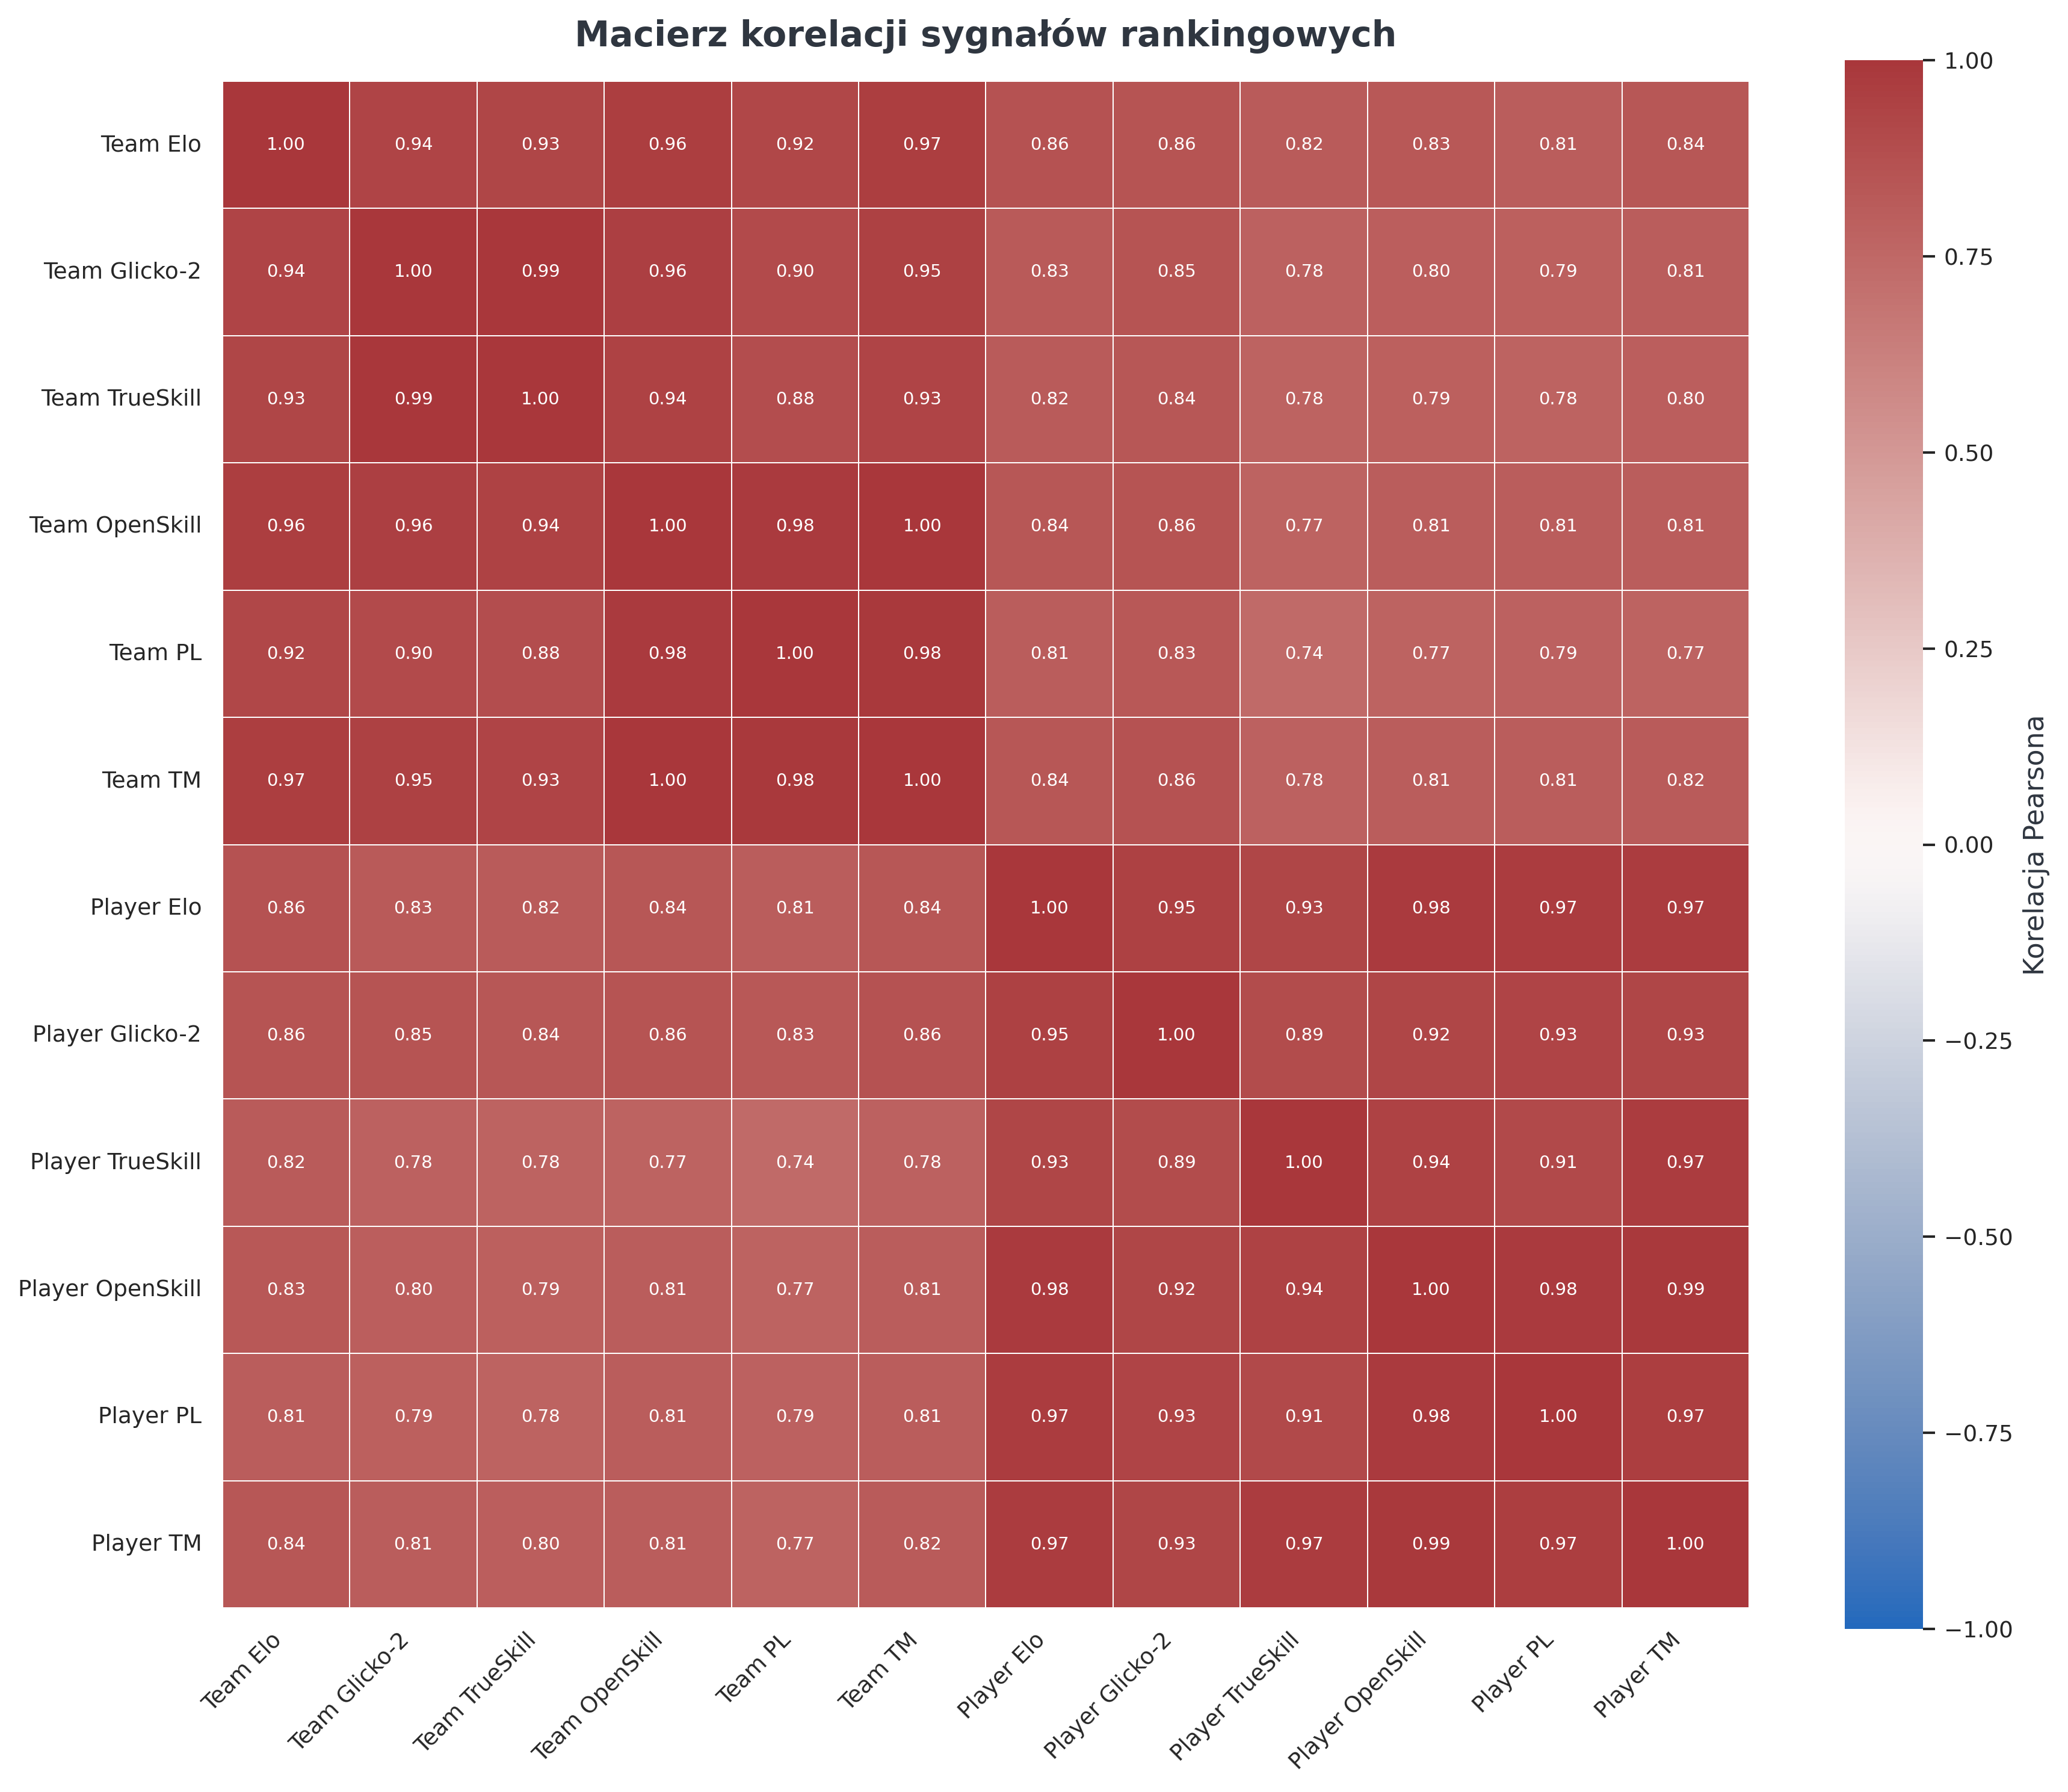
\includegraphics[width=0.9\textwidth]{metamodel_correlation_vif/rating_signal_correlation_heatmap.png}
    \caption{Macierz korelacji głównych sygnałów rankingowych.}
    \label{fig:rating_signal_correlation}
\end{figure}

Macierz na rysunku~\ref{fig:rating_signal_correlation} pokazuje bardzo silną współzależność wielu ratingów. Nie oznacza to, że cechy rankingowe są bezużyteczne; przeciwnie, pokazuje, że zawierają podobny sygnał sportowy. Oznacza jednak, że model liniowy powinien być regularyzowany, a interpretacja pojedynczych współczynników musi być ostrożna.

\subsection{Analiza VIF i konsekwencje dla modelu liniowego}

Drugim krokiem była analiza VIF, czyli variance inflation factor. Wysoki VIF wskazuje na silną współliniowość i może prowadzić do niestabilnych współczynników w modelach liniowych.

\begin{table}[H]
    \centering
    \caption{Najwyższe wartości VIF dla sygnałów rankingowych}
    \label{tab:rating_signal_vif}
    \begin{tabular}{lr}
        \toprule
        Sygnał rankingowy & VIF \\
        \midrule
        Team Thurstone--Mosteller & 337{,}6 \\
        Team OpenSkill & 222{,}3 \\
        Team Glicko-2 & 143{,}4 \\
        Player OpenSkill & 132{,}6 \\
        Player Thurstone--Mosteller & 126{,}4 \\
        Player Plackett--Luce & 124{,}5 \\
        Team TrueSkill & 109{,}4 \\
        Team Plackett--Luce & 106{,}3 \\
        Player Elo & 59{,}7 \\
        Team Elo & 41{,}4 \\
        Player TrueSkill & 25{,}4 \\
        Player Glicko-2 & 13{,}2 \\
        \bottomrule
    \end{tabular}
\end{table}

Wyniki w tabeli~\ref{tab:rating_signal_vif} potwierdzają, że część sygnałów rankingowych jest silnie współliniowa. W pracy nie potraktowano tego jako powodu do ręcznego usunięcia całych rodzin ratingów, ponieważ podobne systemy mogą nadal wnosić niewielkie, ale użyteczne różnice w konkretnych okresach, ligach lub składach. Wniosek z analizy VIF jest zatem metodologiczny: finalny metamodel powinien wykorzystywać regularyzację oraz powinien być oceniany przede wszystkim przez jakość predykcji out-of-time, a nie przez bezpośrednią interpretację pojedynczych współczynników.

Z tego powodu w dalszych eksperymentach zastosowano regresję logistyczną ElasticNet oraz porównano ją z modelami nieliniowymi w procedurze walk-forward. Regularyzacja ElasticNet ogranicza wpływ współliniowości przez zmniejszanie wag podobnych cech i częściową selekcję sygnałów, natomiast bootstrap blokowy sprawdza, czy uzyskana przewaga nie wynika z jednej niestabilnej konfiguracji danych. Analiza VIF pełni więc rolę uzasadnienia wyboru regularyzowanego estymatora i ostrożnej interpretacji wag modelu, a nie osobnego kryterium eliminacji cech.

\section{Dobór długości okna historycznego}

Osobno sprawdzono długość okna historycznego dla pełnego kontekstu drużynowego. Testowano okna W3, W5, W10, W20 oraz W50. Krótsze okna szybciej reagują na zmianę formy, lecz są bardziej podatne na szum pojedynczych meczów. Dłuższe okna są stabilniejsze, ale mogą mieszać aktualną formę z nieaktualnymi składami, patchami lub stylami gry.

\begin{table}[H]
    \centering
    \caption{Wpływ długości okna historycznego na jakość metamodelu}
    \label{tab:metamodel_window_ablation}
    \begin{tabular}{lrrrr}
        \toprule
        Okno & AUC & LogLoss & Brier & ECE \\
        \midrule
        W3 & 0{,}7470 & 0{,}5928 & 0{,}2036 & 0{,}0131 \\
        W5 & 0{,}7476 & 0{,}5924 & 0{,}2035 & 0{,}0108 \\
        W10 & 0{,}7477 & 0{,}5925 & 0{,}2034 & 0{,}0088 \\
        W20 & 0{,}7492 & 0{,}5910 & 0{,}2028 & 0{,}0088 \\
        W50 & 0{,}7489 & 0{,}5915 & 0{,}2030 & 0{,}0124 \\
        \bottomrule
    \end{tabular}
\end{table}

Najniższy LogLoss w tej ablacji uzyskało okno W20. Różnica względem W50 nie jest duża, ale W20 lepiej odpowiada finalnej interpretacji modelu: ma reprezentować aktualną formę, styl i tempo drużyny, bez nadmiernego obciążenia starszymi meczami. Dlatego w dalszych eksperymentach jako główny wariant kontekstu przyjęto W20.

\section{Dobór rodziny estymatora po strojeniu hiperparametrów}

Ostatnim krokiem wyboru architektury było porównanie kilku rodzin modeli na tym samym kompletnym zestawie cech W20-Binomial. Hiperparametry dla każdej rodziny dobrano za pomocą Optuny na chronologicznym zbiorze walidacyjnym. Wyników samej walidacji Optuny nie traktowano jako finalnej tabeli rezultatów; Optuna pełniła funkcję strojenia hiperparametrów. Dopiero dostrojone warianty oceniono w schemacie walk-forward, który lepiej odpowiada rzeczywistemu użyciu modelu w czasie.

Porównano regresję logistyczną ElasticNet, ExtraTrees, LightGBM, HistGradientBoosting oraz małą sieć MLP. Wszystkie modele korzystały z tego samego zestawu cech W20-Binomial i były trenowane w schemacie expanding-window z aktualizacją co 1000 meczów.

\begin{table}[H]
    \centering
    \caption{Porównanie dostrojonych rodzin modeli W20-Binomial w procedurze walk-forward}
    \label{tab:w20_binomial_model_family_comparison}
    \begin{tabular}{lrrrr}
        \toprule
        Model & AUC & LogLoss & Brier & ECE \\
        \midrule
        LR ElasticNet & 0{,}7553 & 0{,}5858 & 0{,}2007 & 0{,}0130 \\
        ExtraTrees & 0{,}7505 & 0{,}5896 & 0{,}2024 & 0{,}0121 \\
        LightGBM & 0{,}7507 & 0{,}5897 & 0{,}2024 & 0{,}0110 \\
        HistGradientBoosting & 0{,}7502 & 0{,}5904 & 0{,}2026 & 0{,}0100 \\
        MLP & 0{,}7456 & 0{,}5952 & 0{,}2046 & 0{,}0201 \\
        \bottomrule
    \end{tabular}
\end{table}

Najniższy LogLoss i najwyższy AUC uzyskała regresja logistyczna ElasticNet. Modele nieliniowe miały miejscami lepsze ECE, lecz zgodnie z hierarchią metryk głównym kryterium wyboru pozostaje LogLoss, ponieważ bezpośrednio mierzy jakość prognozy probabilistycznej i silnie karze błędną pewność.

\begin{figure}[H]
    \centering
    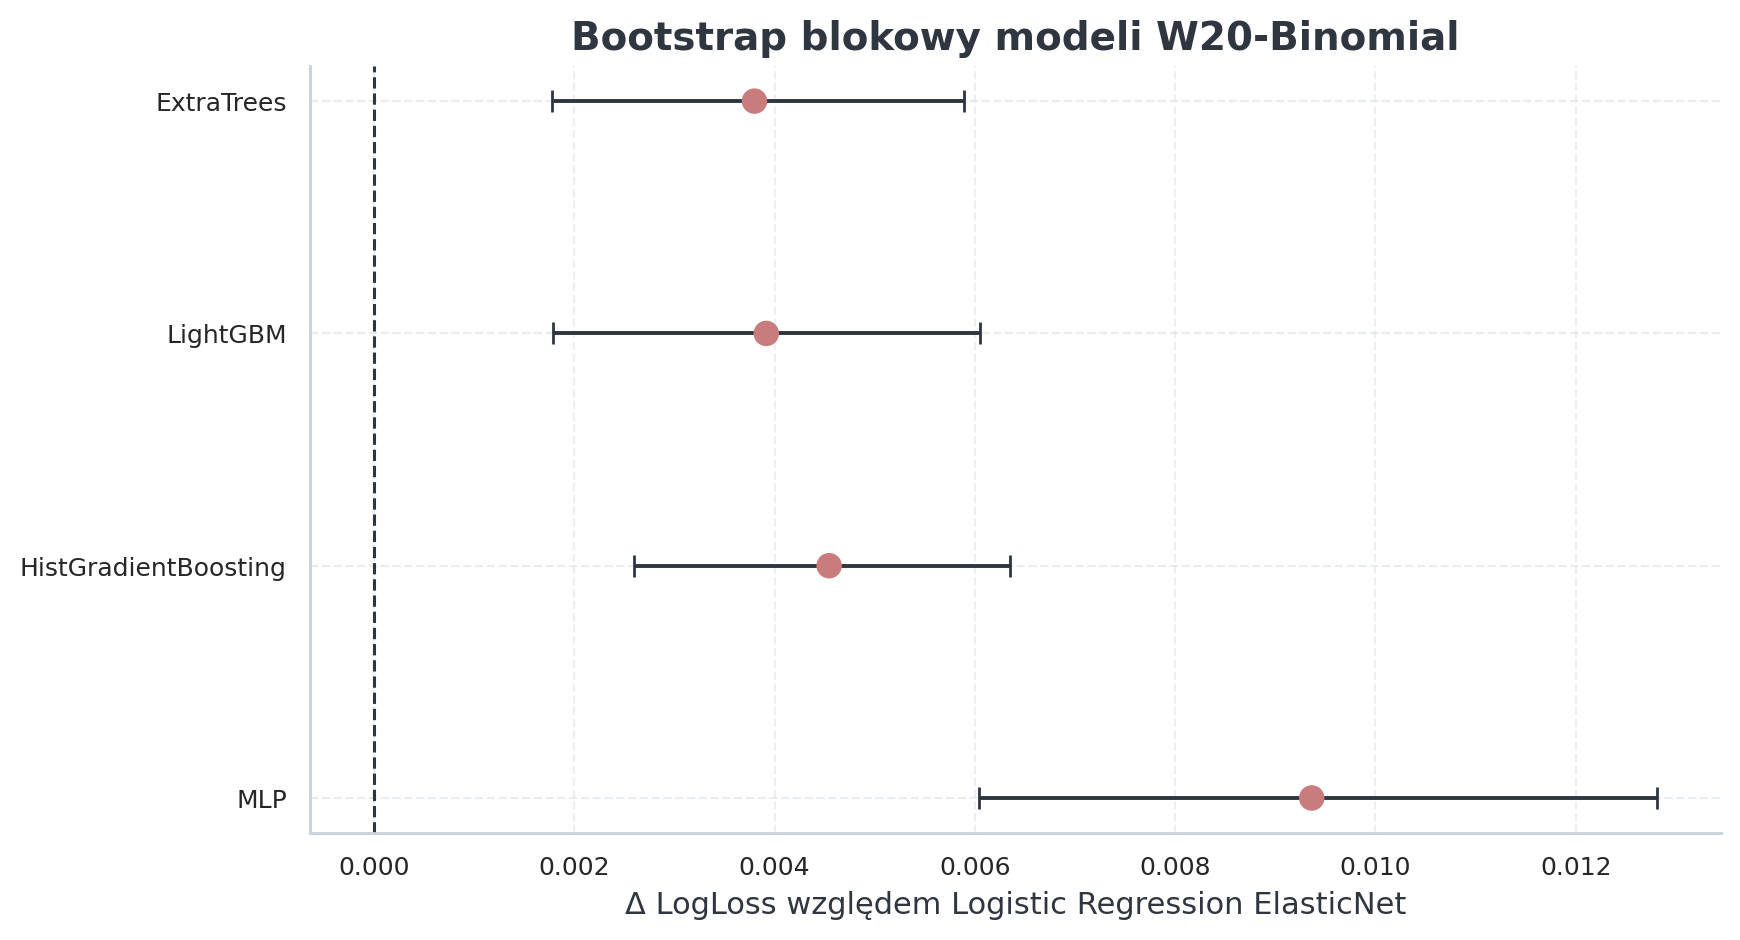
\includegraphics[width=0.92\textwidth]{w20_binomial_all_models_bootstrap/all_models_bootstrap_delta_logloss.png}
    \caption{Miesięczny bootstrap blokowy różnic LogLoss dostrojonych modeli względem regresji logistycznej ElasticNet.}
    \label{fig:w20_binomial_all_models_bootstrap}
\end{figure}

Bootstrap blokowy przedstawiony na rysunku~\ref{fig:w20_binomial_all_models_bootstrap} potwierdza stabilność przewagi modelu liniowego. Wszystkie testowane warianty nieliniowe miały dodatnie przedziały ufności dla różnicy LogLoss względem regresji logistycznej ElasticNet. Różnice wynosiły odpowiednio około 0{,}0038 dla ExtraTrees, 0{,}0039 dla LightGBM, 0{,}0045 dla HistGradientBoosting oraz 0{,}0094 dla MLP. Oznacza to, że wybór regresji logistycznej nie wynika wyłącznie z pojedynczej tabeli metryk, lecz jest stabilny względem miesięcznego resamplingu.

\section{Ablacje finalnego estymatora: masking i sygnał Glicko-2}

Po wyborze regresji logistycznej ElasticNet jako finalnej rodziny estymatora przeprowadzono dodatkowe ablacje wyjaśniające, z których sygnałów korzysta model. Taka kolejność jest istotna: najpierw wybrano klasę modelu na kompletnym zestawie cech W20-Binomial, a dopiero następnie sprawdzono wrażliwość wybranego estymatora na maskowanie i usuwanie wybranych grup rankingowych. Szczególnie ważny był test zależności od rodziny Glicko-2, ponieważ w rozdziale rankingowym Player Glicko-2 był najlepszym pojedynczym sygnałem.

\begin{table}[H]
    \centering
    \caption{Masking i ablacja sygnału Player Glicko-2 w modelu kontekstowym}
    \label{tab:logistic_masking_ablation}
    \begin{tabular}{lrrrr}
        \toprule
        Wariant & AUC & LogLoss & ECE & $\Delta$ LogLoss \\
        \midrule
        Pełny model kontekstowy & 0{,}7555 & 0{,}5855 & 0{,}0118 & 0{,}0000 \\
        G2 + context & 0{,}7551 & 0{,}5861 & 0{,}0102 & 0{,}0005 \\
        Mask all 10\% & 0{,}7537 & 0{,}5868 & 0{,}0085 & 0{,}0012 \\
        Mask G2 10\% & 0{,}7527 & 0{,}5875 & 0{,}0089 & 0{,}0020 \\
        Mask G2 30\% & 0{,}7516 & 0{,}5884 & 0{,}0110 & 0{,}0028 \\
        No player\_gl & 0{,}7501 & 0{,}5898 & 0{,}0130 & 0{,}0042 \\
        No G2 family & 0{,}7470 & 0{,}5925 & 0{,}0119 & 0{,}0070 \\
        \bottomrule
    \end{tabular}
\end{table}

Eksperyment potwierdza, że Player Glicko-2 jest najważniejszym pojedynczym sygnałem, ale pełny model korzysta również z informacji zastępczej zawartej w pozostałych rankingach. Maskowanie cech w danych treningowych nie poprawiło wyniku, dlatego nie zostało włączone do finalnego estymatora. Ablacja pełni jednak ważną funkcję kontrolną: pokazuje, że model nie jest arbitralną czarną skrzynką, lecz wykorzystuje przewidywalną strukturę sygnałów rankingowych.

Osobno sprawdzono, czy do finalnego wejścia warto dodać predykcje i parametry rankingów drużynowych. Wariant rozszerzony Player+Team W20-Binomial uzyskał minimalnie niższy LogLoss niż wariant player-based, ale różnica była bardzo mała i nie została potwierdzona w miesięcznym bootstrapie blokowym. Wynik przedstawiono w tabeli~\ref{tab:player_team_ablation}. Z tego powodu finalny model zachowuje prostszą strukturę: komponent rankingowy opiera się na sygnałach zawodniczych, natomiast informacja drużynowa jest reprezentowana przez pełny kontekst historyczny W20.

\begin{table}[H]
    \centering
    \caption{Ablacja dodania rankingów drużynowych do finalnego wejścia W20-Binomial}
    \label{tab:player_team_ablation}
    \begin{tabular}{lrrrr}
        \toprule
        Wariant & AUC & LogLoss & Brier & ECE \\
        \midrule
        Player-based W20-Binomial & 0{,}7553 & 0{,}5858 & 0{,}2007 & 0{,}0131 \\
        Player+Team W20-Binomial & 0{,}7554 & 0{,}5857 & 0{,}2007 & 0{,}0144 \\
        \bottomrule
    \end{tabular}
\end{table}

W miesięcznym bootstrapie blokowym różnica $\Delta=\mathrm{LogLoss}_{\mathrm{Player+Team}}-\mathrm{LogLoss}_{\mathrm{Player}}$ wyniosła $-0{,}0001$, a przedział ufności 95\% był równy $[-0{,}0002,\ 0{,}0020]$. Ponieważ przedział obejmuje zero, dodatkowe cechy team-based potraktowano jako zwiększenie złożoności bez stabilnej poprawy jakości predykcji.

\begin{figure}[H]
    \centering
    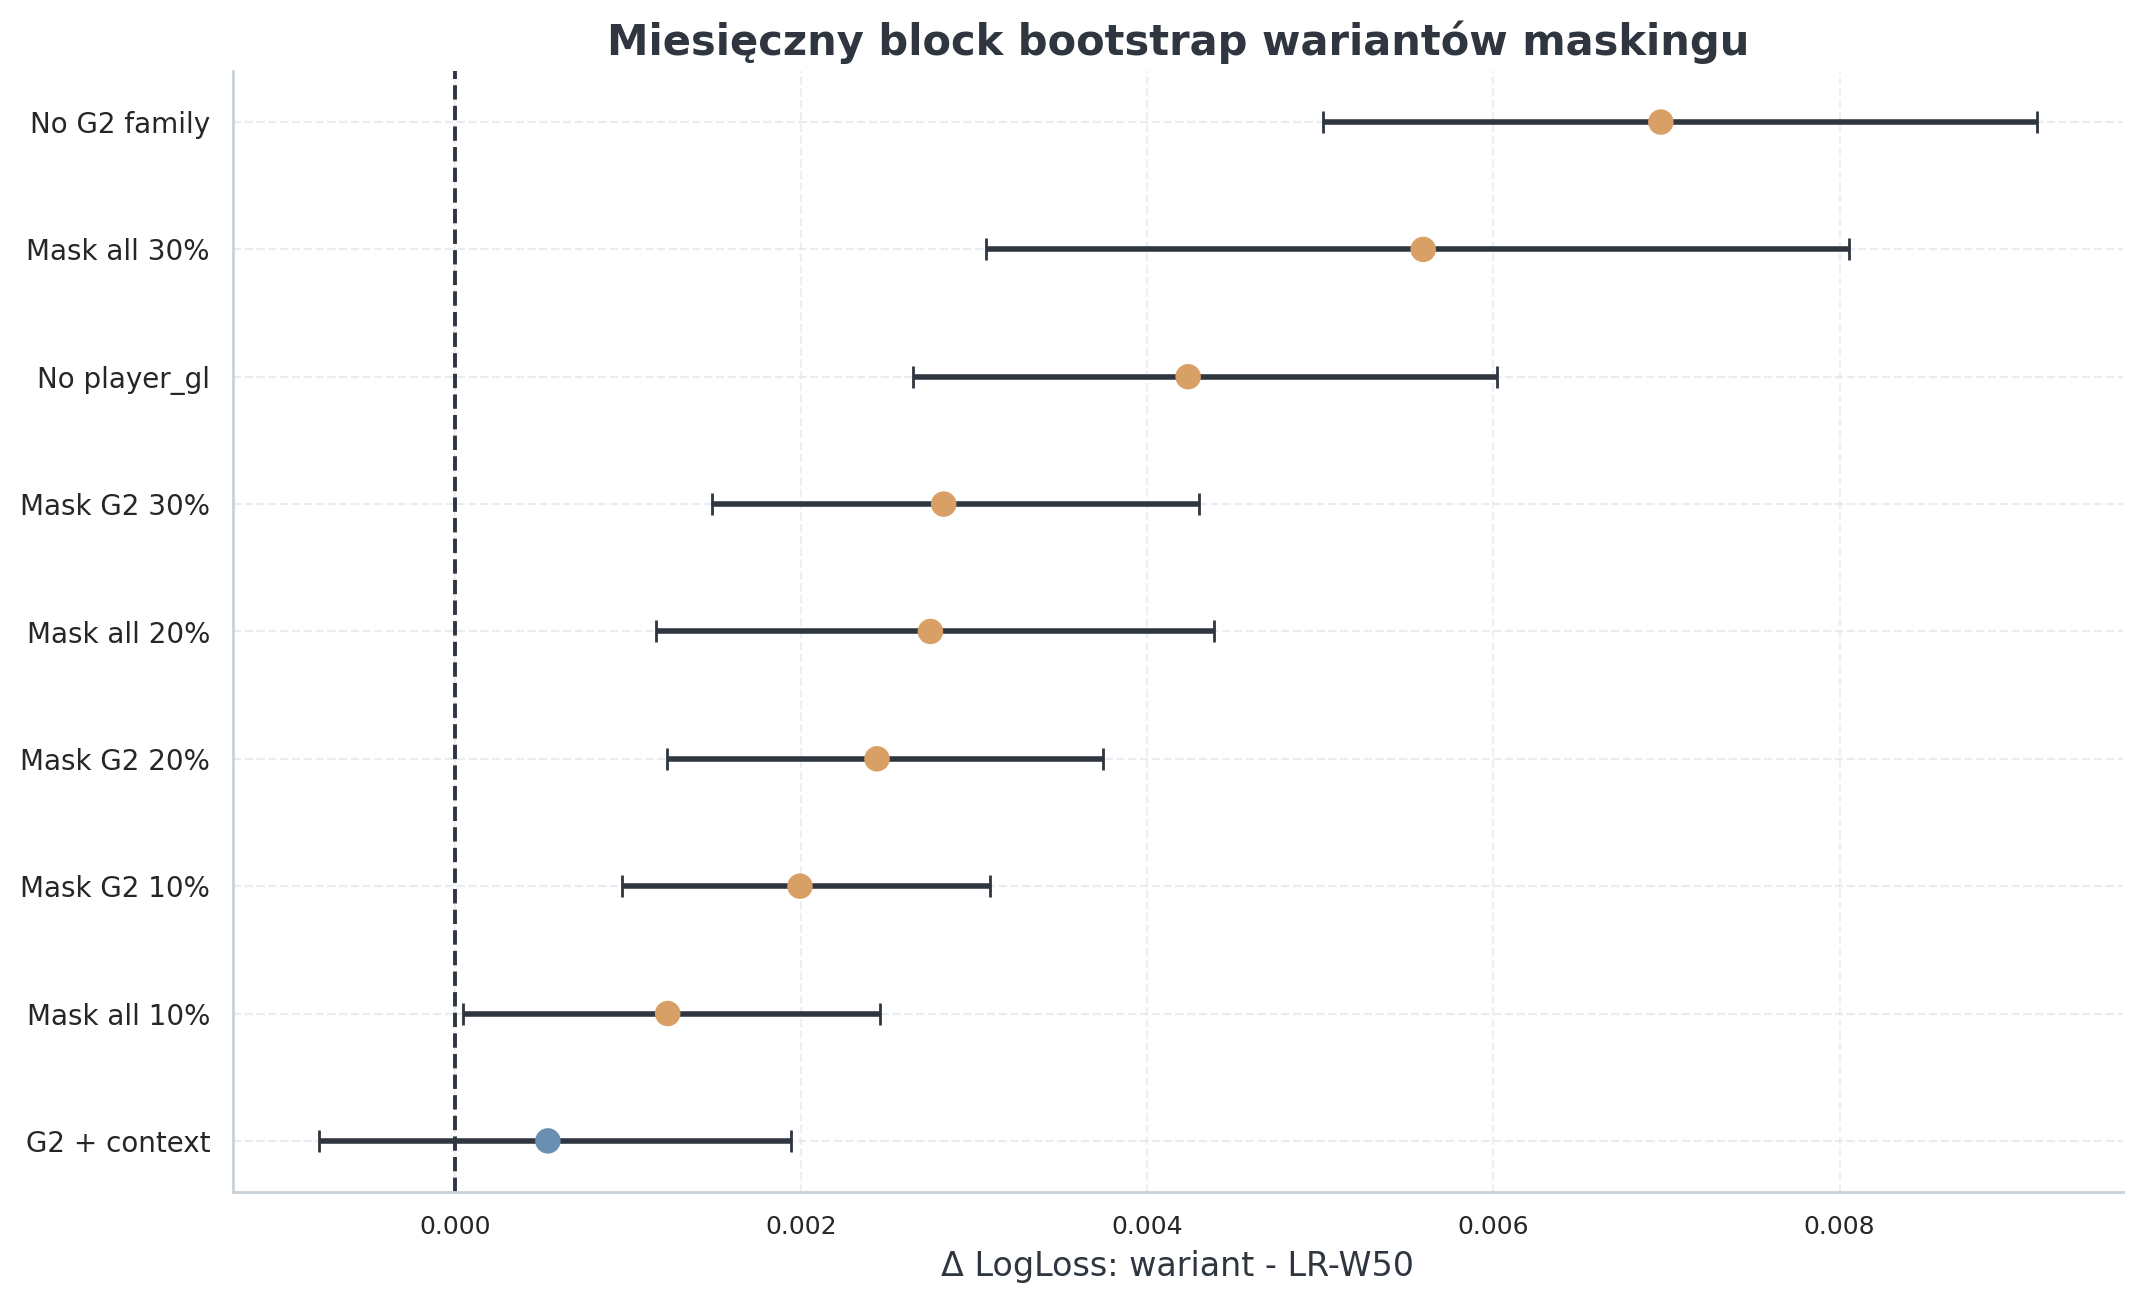
\includegraphics[width=0.9\textwidth]{logistic_masking_ablation_bootstrap/masking_monthly_block_bootstrap_ci.png}
    \caption{Miesięczny bootstrap blokowy różnic LogLoss wariantów maskingu względem pełnego modelu kontekstowego.}
    \label{fig:masking_block_bootstrap}
\end{figure}

\section{Symetryzacja kolejności drużyn}

\subsection{Źródło asymetrii technicznej}

Regresja logistyczna trenowana na wektorze cech zależnym od kolejności stron meczu generuje predykcję dla zdarzenia, że wygra strona zapisana jako Team 1. Problem ten jest technicznie naturalny, ponieważ dane wejściowe mają postać różnic lub par cech Team 1--Team 2. Jednocześnie z perspektywy sportowej prawdopodobieństwo powinno spełniać warunek antysymetrii: jeżeli ten sam mecz zostanie zapisany w odwróconej kolejności, to prawdopodobieństwo zwycięstwa pierwszej strony powinno być dopełnieniem poprzedniej predykcji.

\subsection{Procedura uśredniania predykcji}

W praktyce sprawdzono, że surowy estymator nie jest idealnie niewrażliwy na kolejność drużyn. Dla każdego meczu wygenerowano więc dwie predykcje: predykcję w oryginalnej orientacji oraz predykcję po zamianie stron. Predykcję po zamianie stron przeliczono z powrotem na prawdopodobieństwo zwycięstwa pierwotnej strony, a następnie uśredniono oba oszacowania:

\begin{equation}
    p_{sym}(A>B) = \frac{p_{orig}(A>B) + \left(1 - p_{swap}(B>A)\right)}{2}.
    \label{eq:symmetrized_prediction}
\end{equation}

Tak zdefiniowany wariant zachowuje informację wyuczoną przez regresję logistyczną, ale ogranicza artefakt wynikający z arbitralnego zapisu meczu. Diagnostyka wrażliwości kolejności wykazała średnią bezwzględną różnicę prawdopodobieństw równą około 0{,}0287, medianę 0{,}0237 oraz maksimum 0{,}2113. Po symetryzacji surowy model uzyskał AUC 0{,}7561 i LogLoss 0{,}5858, nieznacznie poprawiając rozróżnianie względem predykcji w oryginalnej orientacji. Wniosek z tej analizy jest metodologiczny: model końcowy powinien respektować symetrię problemu, nawet jeżeli sama poprawa metryk jest niewielka.

\section{Kalibracja prawdopodobieństw}

\subsection{Schemat expanding-window}

Ponieważ celem pracy jest predykcja probabilistyczna, końcowy wariant modelu poddano dodatkowej analizie kalibracji. Porównano predykcje surowe, kalibrację Platta oraz kalibrację izotoniczną. Obie metody były stosowane w schemacie expanding-window: kalibrator dla danego folda uczono wyłącznie na wcześniejszych foldach, bez wykorzystania przyszłych obserwacji. Dzięki temu kalibracja zachowuje chronologiczny charakter ewaluacji.

\subsection{Porównanie Platta i kalibracji izotonicznej}

Kalibracja Platta polegała na dopasowaniu regresji logistycznej do logitu surowych prawdopodobieństw modelu. Jej zaletą jest mała liczba parametrów i odporność na mniejsze próbki kalibracyjne. Kalibracja izotoniczna jest bardziej elastyczna, ale może łatwiej dopasować lokalny szum, szczególnie przy dryfie danych i nierównej liczbie obserwacji w kolejnych okresach.

\begin{table}[H]
    \centering
    \caption{Porównanie wariantów symetryzacji i kalibracji na wspólnej próbie rynkowej}
    \label{tab:symmetry_calibration_comparison}
    \small
    \begin{tabular}{lrrrr}
        \toprule
        Wariant & AUC & LogLoss & Brier & ECE \\
        \midrule
        Symetryczny + Platt expanding & 0{,}7551 & 0{,}5854 & 0{,}2007 & 0{,}0100 \\
        Oryginalny + Platt expanding & 0{,}7542 & 0{,}5862 & 0{,}2010 & 0{,}0098 \\
        Symetryczny surowy & 0{,}7551 & 0{,}5867 & 0{,}2011 & 0{,}0193 \\
        Oryginalny surowy & 0{,}7543 & 0{,}5868 & 0{,}2011 & 0{,}0125 \\
        Symetryczny + isotonic expanding & 0{,}7532 & 0{,}5901 & 0{,}2013 & 0{,}0097 \\
        Oryginalny + isotonic expanding & 0{,}7519 & 0{,}5906 & 0{,}2018 & 0{,}0104 \\
        \bottomrule
    \end{tabular}
\end{table}

\begin{figure}[H]
    \centering
    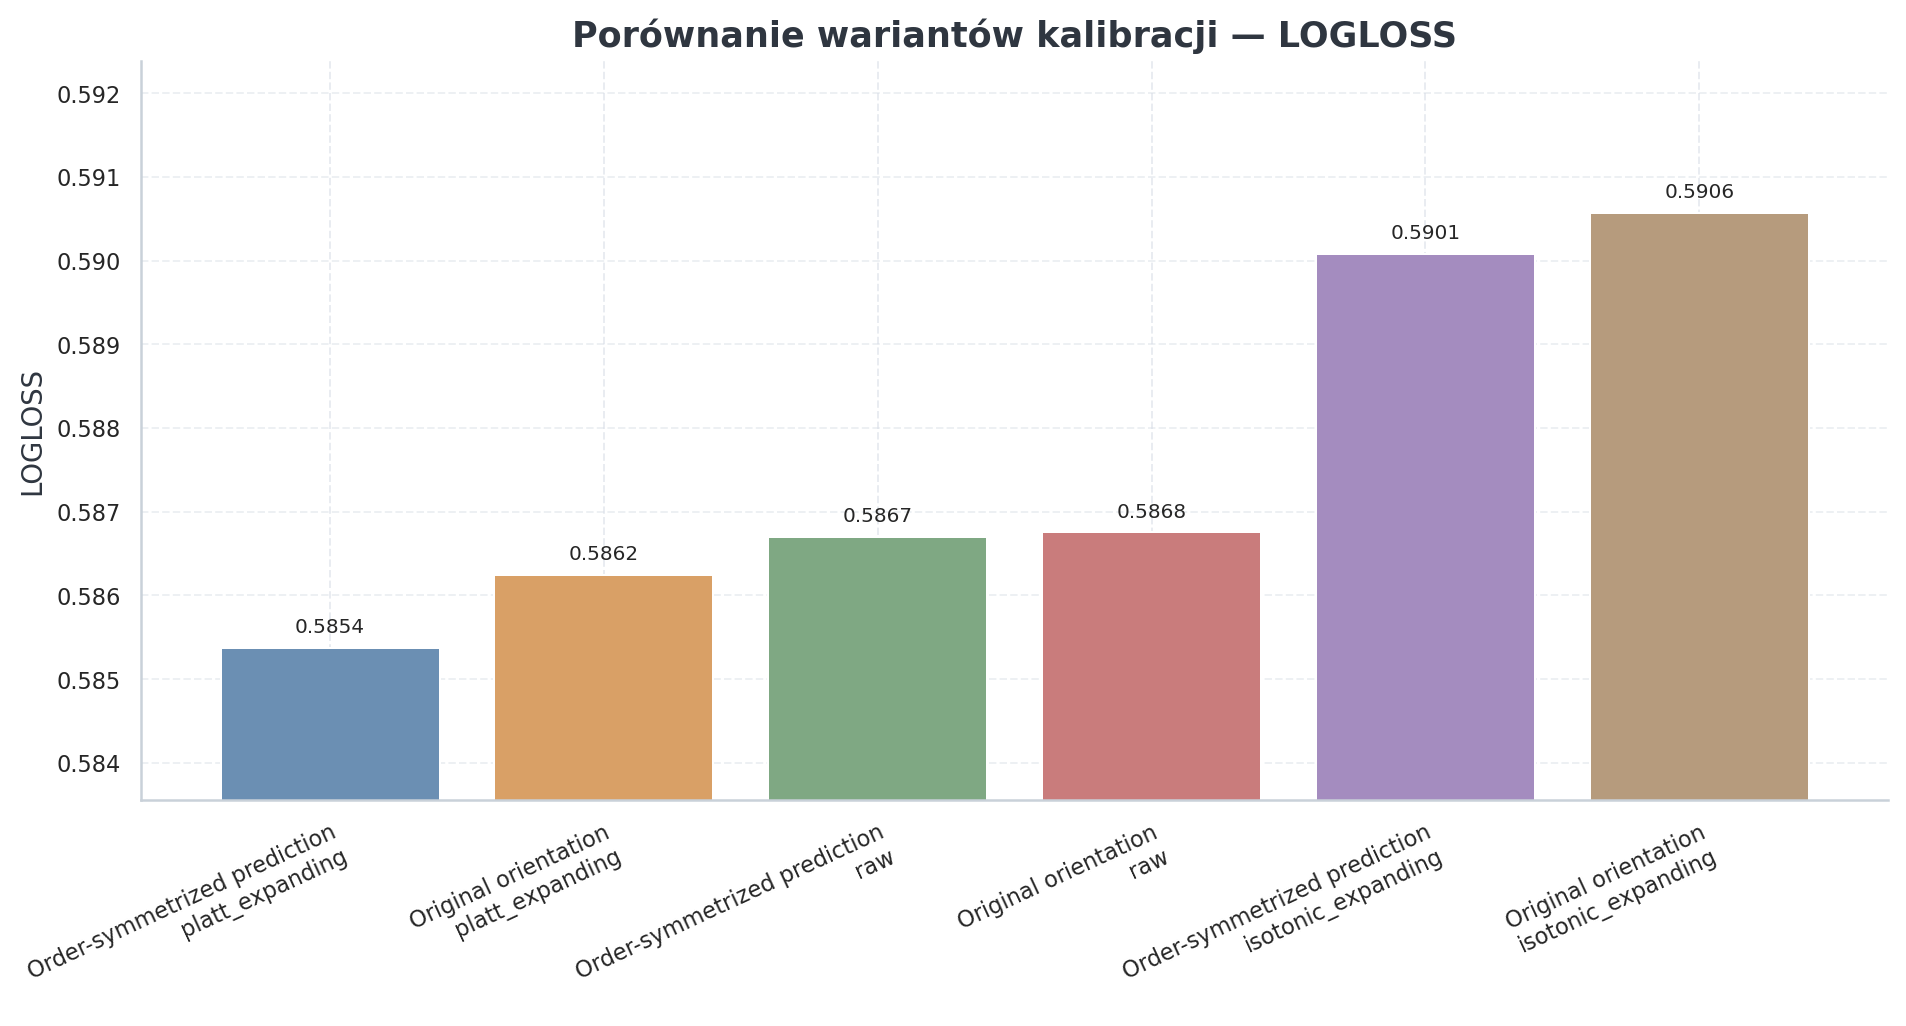
\includegraphics[width=0.92\textwidth]{final_symmetric_calibrated_market_comparison/final_symmetric_calibrated_calibration_logloss.png}
    \caption{Porównanie wariantów symetryzacji i kalibracji według LogLoss na wspólnej próbie rynkowej.}
    \label{fig:final_calibration_logloss}
\end{figure}

\begin{figure}[H]
    \centering
    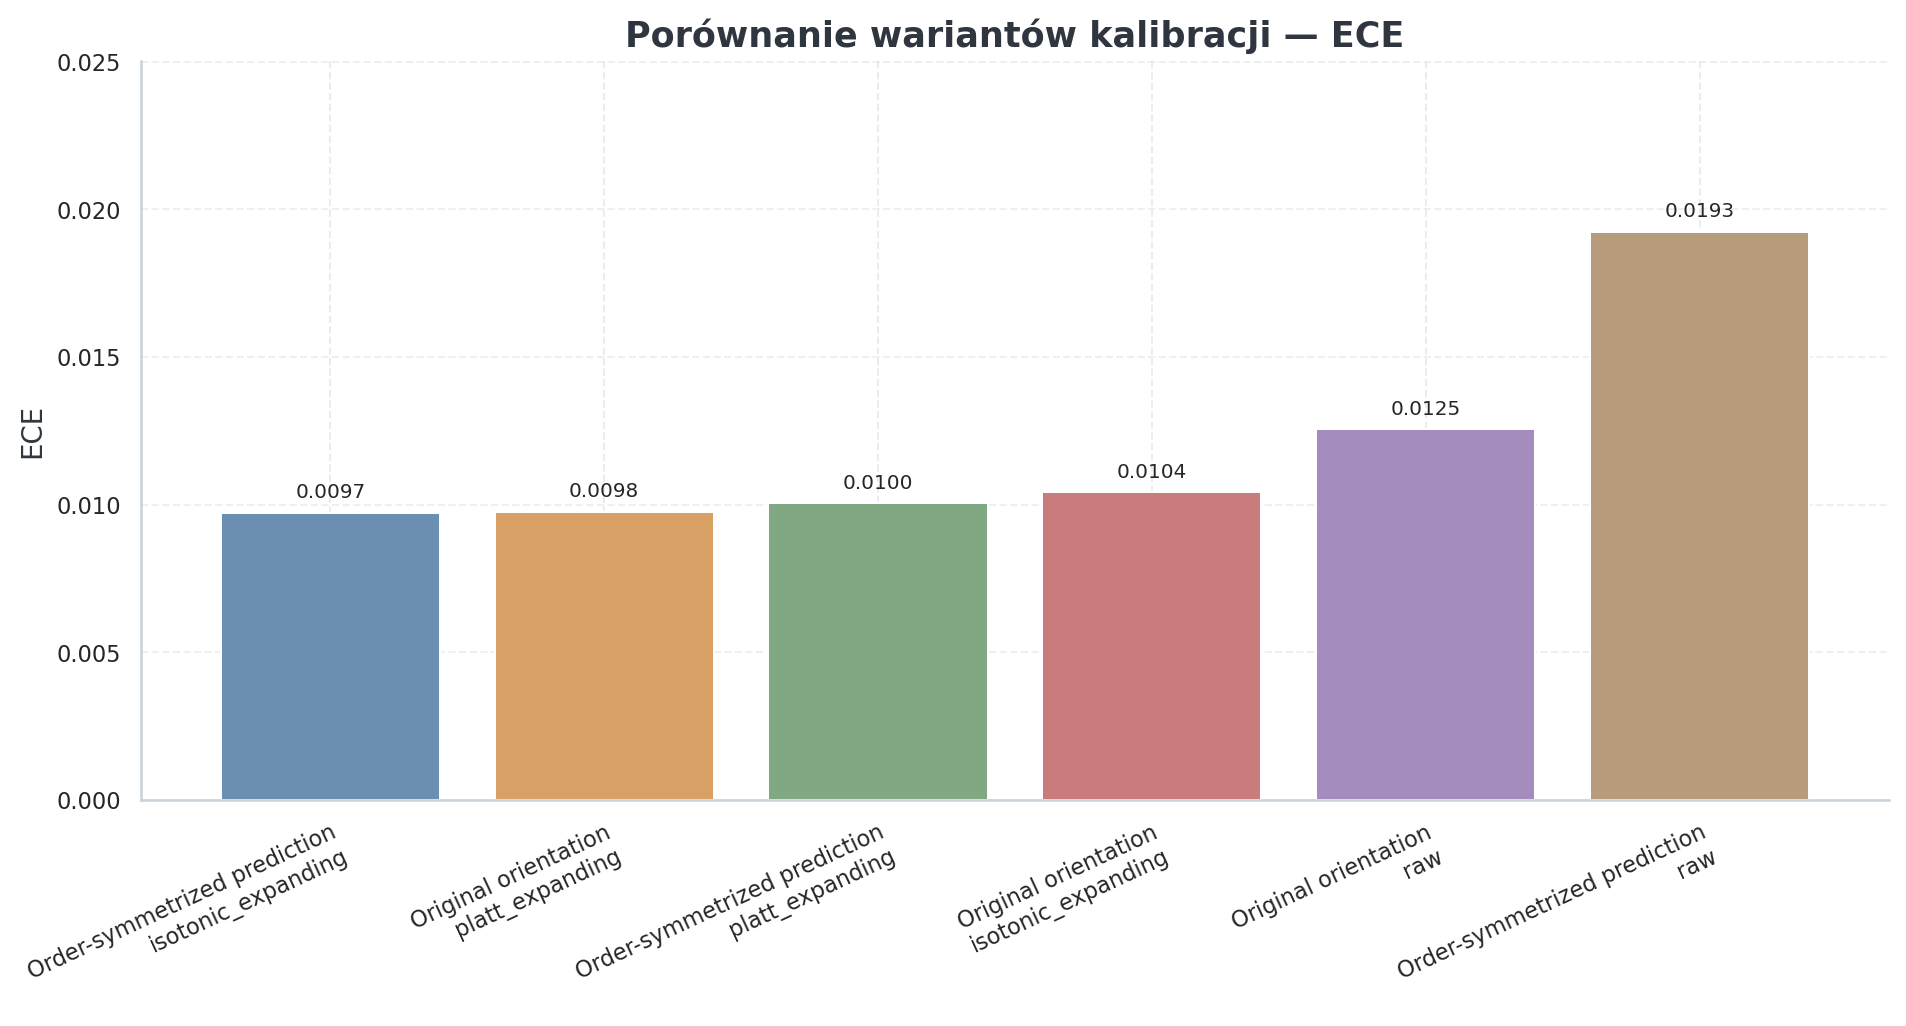
\includegraphics[width=0.92\textwidth]{final_symmetric_calibrated_market_comparison/final_symmetric_calibrated_calibration_ece.png}
    \caption{Porównanie wariantów symetryzacji i kalibracji według ECE na wspólnej próbie rynkowej.}
    \label{fig:final_calibration_ece}
\end{figure}

Najniższy LogLoss uzyskał wariant symetryczny z kalibracją Platta. Kalibracja izotoniczna dawała bardzo niskie ECE, ale pogarszała LogLoss i AUC. Zgodnie z hierarchią metryk przyjętą w pracy wybrano więc wariant Platta: poprawiał kalibrację względem surowego modelu, a jednocześnie nie obniżał jakości probabilistycznej mierzonej główną metryką. Ostateczny model kierowany do porównania z benchmarkami rynkowymi to \textbf{skalibrowany symetryczny LR-ElasticNet-W20-Binomial}.

\section{Wnioski z etapu metamodelowania}

Etap metamodelowania prowadzi do sześciu głównych wniosków. Po pierwsze, cechy zawodnicze pozostają najważniejszą podstawą predykcji, a Player Glicko-2 jest najsilniejszym pojedynczym sygnałem rankingowym. Po drugie, pełny kontekst W20 uzupełnia rankingi o informacje o aktualnej formie, stylu, ekonomii, obiektach i tempie gry. Po trzecie, format serii Bo1/Bo3/Bo5 najlepiej uwzględnić strukturalnie przez transformację dwumianową prawdopodobieństw rankingowych. Po czwarte, mimo przetestowania modeli drzewiastych i MLP, najlepiej generalizującym estymatorem okazała się regularyzowana regresja logistyczna ElasticNet. Po piąte, finalny model powinien respektować symetrię problemu względem kolejności drużyn. Po szóste, kalibracja Platta poprawia jakość prawdopodobieństw bez pogorszenia LogLoss, dlatego została użyta w wariancie końcowym.

Najważniejszym rezultatem tego rozdziału jest wybór modelu głównego do porównania z benchmarkami bukmacherskimi: \textbf{skalibrowanego symetrycznego LR-ElasticNet-W20-Binomial}. Model ten będzie w następnym rozdziale oceniony na wspólnej próbie meczów posiadających zarówno dane sportowe, jak i kursy bukmacherskie.

\input{chapters/06_ocena_i_porownanie_z_bukmacherami}
\chapter{Dyskusja}

\section{Interpretacja najważniejszych wyników}

\subsection{Znaczenie modelowania na poziomie zawodników}

Najbardziej spójnym wynikiem pracy jest przewaga systemów rankingowych liczonych na poziomie zawodników nad rankingami liczonymi wyłącznie na poziomie organizacji. Jest to zgodne ze specyfiką profesjonalnego \textit{League of Legends}. Drużyna nie jest stabilną jednostką w takim samym sensie jak klub w wielu tradycyjnych dyscyplinach sportowych: składy zmieniają się pomiędzy splitami, zawodnicy przechodzą między regionami, a siła organizacji może szybko spaść lub wzrosnąć po transferach. Ranking drużynowy agreguje te zmiany z opóźnieniem, natomiast ranking zawodniczy może przenosić część informacji o jakości gracza po zmianie zespołu.

Nie oznacza to, że sama suma ratingów zawodników w pełni opisuje siłę drużyny. Wyniki metamodelu pokazują raczej, że ratingi zawodnicze są najlepszym fundamentem, ale wymagają uzupełnienia o kontekst historyczny i informacje o formacie serii. W praktyce pięciu silnych zawodników nie zawsze tworzy równie silny zespół, a krótko- i średnioterminowa forma może wpływać na wynik niezależnie od długookresowej oceny siły.

\subsection{Rola metamodelu W20-Binomial}

Metamodel W20-Binomial poprawił jakość probabilistyczną względem najlepszego pojedynczego rankingu. Interpretacyjnie oznacza to, że predykcja meczu nie powinna opierać się wyłącznie na jednym systemie ratingowym. Różne rodziny rankingów opisują podobną ukrytą siłę sportową, ale robią to z inną dynamiką aktualizacji i innym sposobem traktowania niepewności. Połączenie tych sygnałów z kroczącymi statystykami drużynowymi pozwala modelowi odróżnić samą siłę składu od bieżącej formy, stylu gry i kontekstu serii.

Wybór regresji logistycznej ElasticNet jako najlepszego estymatora wskazuje, że zasadnicza część informacji była już zawarta w skonstruowanych cechach. Bardziej złożone modele nieliniowe nie poprawiły LogLoss, mimo że miały większą elastyczność. W tym sensie wynik wspiera podejście inżynierskie oparte na starannej konstrukcji cech, kontroli chronologii i regularyzacji, a nie wyłącznie na zwiększaniu złożoności estymatora.

\subsection{Symetryzacja i kalibracja jako końcowe uporządkowanie modelu}

Końcowa symetryzacja oraz kalibracja Platta przyniosły niewielką, ale stabilną poprawę względem surowego wariantu regresji logistycznej. Skala tej poprawy nie powinna być interpretowana jako przełomowy skok jakościowy. Jej znaczenie jest przede wszystkim metodologiczne: model końcowy lepiej respektuje symetrię problemu, w którym zamiana kolejności drużyn nie powinna zmieniać sensu predykcji, oraz generuje bardziej wiarygodne prawdopodobieństwa.

Warto podkreślić, że kalibracja izotoniczna uzyskała bardzo dobre wartości ECE, ale pogorszyła LogLoss i AUC. Z tego powodu nie została wybrana jako wariant finalny. Decyzja ta jest konsekwencją hierarchii metryk przyjętej w pracy: głównym kryterium jest jakość probabilistyczna mierzona LogLoss, natomiast ECE pełni funkcję diagnostyczną. Skalowanie Platta okazało się lepszym kompromisem pomiędzy kalibracją a stabilnością predykcji.

\section{Interpretacja porównania z rynkiem bukmacherskim}

\subsection{Rynek jako silny benchmark probabilistyczny}

Kursy bukmacherskie są trudnym punktem odniesienia, ponieważ agregują wiele źródeł informacji: modele analityczne, wiedzę ekspertów, reakcje uczestników rynku oraz aktualizacje cen przed meczem. Szczególnie kurs zamknięcia może zawierać informacje niedostępne w danych sportowych wykorzystanych w tej pracy. Z tego powodu porównanie z Market Close jest bardziej wymagające niż porównanie z prostym benchmarkiem rankingowym.

Finalny model uzyskał niższy LogLoss zarówno od Market Open, jak i Market Close na wspólnej próbie historycznej. Wynik ten jest istotny, ponieważ wskazuje, że połączenie ratingów zawodniczych i kontekstu historycznego może przypisywać wynikom prawdopodobieństwa konkurencyjne względem publicznego benchmarku rynkowego. Jednocześnie przewaga ta powinna być interpretowana ostrożnie: dotyczy konkretnej próby, konkretnego sposobu normalizacji kursów i konkretnego horyzontu danych.

\subsection{Granice wniosku rynkowego}

Niższy LogLoss od benchmarku kursowego nie jest równoznaczny z możliwością osiągnięcia zysku z zakładów. Ewaluacja probabilistyczna i strategia finansowa są odrębnymi problemami. Analiza finansowa wymagałaby uwzględnienia marży, podatków, limitów, płynności, dostępności kursów w czasie rzeczywistym, opóźnień wykonania oraz reguł zarządzania ryzykiem. Te elementy nie były przedmiotem pracy.

Dlatego właściwy wniosek jest węższy: na badanej próbie historycznej model sportowy uzyskał lepsze metryki probabilistyczne niż znormalizowane prawdopodobieństwa implikowane przez kursy. Jest to wynik dotyczący jakości predykcyjnej, a nie ekonomicznej przewagi nad rynkiem.

\section{Ograniczenia badania}

\subsection{Zakres i reprezentatywność danych}

Pierwszym ograniczeniem jest zależność wyników od dostępnych źródeł danych. Dane GOL.GG dostarczają bogatego opisu sportowego, ale nie obejmują wszystkich czynników wpływających na wynik meczu. W szczególności brakuje informacji jakościowych o problemach organizacyjnych, chorobach, treningach, komunikacji drużyn, przygotowaniu strategicznym oraz szczegółowym stanie mety w danym patchu. Część tych informacji może być pośrednio uwzględniana przez rynek kursów, ale nie występuje jawnie w zbiorze sportowym.

Drugim ograniczeniem jest fakt, że końcowa próba rynkowa obejmuje tylko mecze posiadające kursy bukmacherskie. Jest to konieczne dla uczciwego porównania z rynkiem, ale zawęża interpretację wyników. Mecze z kursami mogą różnić się od całej populacji meczów GOL.GG: częściej dotyczą ważniejszych lig, bardziej rozpoznawalnych drużyn i spotkań o większym zainteresowaniu.

\subsection{Dryf czasowy i zmiany środowiska gry}

\textit{League of Legends} jest środowiskiem niestacjonarnym. Aktualizacje gry, zmiany mety, przebudowy składów i zmiany formatu rozgrywek mogą wpływać na zależności obserwowane w danych historycznych. Procedura walk-forward ogranicza ryzyko przecieku informacji z przyszłości, ale nie usuwa problemu dryfu danych. Model oceniony historycznie może wymagać okresowej aktualizacji i ponownej walidacji w kolejnych sezonach.

Szczególnie trudne są okresy po dużych zmianach patcha lub po przerwach między sezonami, gdy dotychczasowe ratingi i cechy historyczne mogą słabiej opisywać aktualną siłę drużyn. Z tego powodu wyniki należy traktować jako ocenę na analizowanym horyzoncie, a nie jako gwarancję stałej skuteczności w przyszłości.

\subsection{Ograniczenia konstrukcji cech}

Model wykorzystuje historyczny kontekst W20, rankingowe predykcje bazowe, miary niepewności oraz korektę formatu serii. Nie wykorzystuje natomiast pełnego opisu draftu bohaterów ani szczegółowych interakcji pomiędzy rolami. W praktyce siła drużyny może zależeć od dopasowania stylów gry, synergii zawodników, preferencji bohaterów i zdolności adaptacji do przeciwnika. Te elementy są tylko częściowo reprezentowane przez statystyki historyczne.

Ograniczeniem jest również agregacja informacji na poziomie drużyny i zawodników. Ranking zawodniczy poprawia opis transferów, ale nie modeluje wprost relacji pomiędzy konkretną piątką graczy. Dwie drużyny o podobnej sumarycznej sile zawodników mogą różnić się zgraniem, komunikacją lub dopasowaniem ról. To wskazuje na potencjalną wartość przyszłych cech opisujących stabilność składu i doświadczenie wspólnej gry.

\section{Implikacje dla dalszych badań}

\subsection{Rozszerzenie danych przedmeczowych}

Najbardziej naturalnym kierunkiem rozwoju jest rozszerzenie danych o informacje dostępne przed meczem, ale nieuwzględnione w obecnym zbiorze. Szczególnie ważny może być draft bohaterów, kontekst patcha, absencje, zmiany składu oraz bardziej szczegółowe informacje o historii wspólnej gry zawodników. Takie dane mogłyby poprawić model zwłaszcza w meczach, w których różnica ratingów jest niewielka.

\subsection{Walidacja przyszłościowa}

Drugim kierunkiem jest rygorystyczna walidacja przyszłościowa. Najsilniejszym testem byłoby zamrożenie procesu konstrukcji cech, hiperparametrów i procedury kalibracji, a następnie ocena na pełnym kolejnym sezonie, który nie był użyty ani w eksploracji, ani w doborze modelu. Pozwoliłoby to lepiej ocenić odporność metamodelu na dryf danych i zmiany środowiska gry.

\subsection{Lepsze modelowanie składu i synergii}

Trzecim kierunkiem jest dokładniejsze modelowanie składu. Obecna praca pokazuje, że poziom zawodniczy jest ważniejszy niż sama nazwa drużyny, ale nie wyczerpuje problemu. Można rozważyć cechy opisujące stabilność piątki, liczbę wspólnie rozegranych meczów, zmiany ról, doświadczenie międzynarodowe oraz zgodność stylów gry. Takie cechy mogłyby pomóc odróżnić drużyny złożone z indywidualnie silnych graczy od zespołów rzeczywiście stabilnych taktycznie.

\section{Podsumowanie dyskusji}

Wyniki pracy wskazują, że połączenie rankingów zawodniczych, kontekstu historycznego i prostego regularyzowanego metamodelu może skutecznie przewidywać profesjonalne mecze \textit{League of Legends}. Najważniejsza wartość pracy nie polega na pojedynczym dużym skoku metryki, lecz na spójnym procesie: od systemów rankingowych, przez kontrolę chronologii i metamodelowanie, po końcową kalibrację oraz porównanie z rynkiem. Ograniczenia dotyczą głównie zakresu danych, dryfu czasowego oraz braku części informacji jakościowych. Wnioski należy więc traktować jako dowód skuteczności przyjętej metodologii na historycznej próbie, a nie jako pełne rozwiązanie problemu predykcji esportowej.

\input{chapters/07_zakonczenie}

% Kolejne rozdziały zostaną dodane w osobnych plikach:
% Dalsze załączniki i wykazy zostaną dodane po finalnej redakcji.

\printbibliography

\listoffigures
\listoftables

\end{document}
